\documentclass[11pt,oneside]{book}
\usepackage[T1]{fontenc}
\usepackage[utf8]{inputenc}
\usepackage{lmodern}
\usepackage[margin=0.82in,headheight=15pt]{geometry}
\usepackage{microtype}
\usepackage{amsmath,amssymb,amsthm,mathtools}
\usepackage{bm}
\usepackage{graphicx}
\usepackage{booktabs,longtable,tabularx,array,multirow}
\usepackage{enumitem}
\usepackage{xcolor}
\usepackage{caption}
\usepackage{subcaption}
\usepackage{float}
\usepackage[section]{placeins}
\usepackage{fancyhdr}
\usepackage{hyperref}
\usepackage[nameinlink,noabbrev]{cleveref}
\usepackage[most]{tcolorbox}
\usepackage{listings}
\usepackage{url}

\definecolor{ink}{HTML}{17202A}
\definecolor{blue}{HTML}{2E86AB}
\definecolor{teal}{HTML}{2A9D8F}
\definecolor{orange}{HTML}{F4A261}
\definecolor{red}{HTML}{E76F51}
\definecolor{purple}{HTML}{6C5CE7}
\definecolor{paper}{HTML}{FBFBF8}
\definecolor{softgray}{HTML}{EEF1F3}

\hypersetup{
  colorlinks=true,
  linkcolor=purple,
  citecolor=teal,
  urlcolor=blue,
  pdftitle={Projector-Resolved Hodge Calculus: Complete Fermat Fourfold and CM Half-Twist Edition},
  pdfauthor={Komorebi P.},
  pdfsubject={Projector Hodge calculus, Fermat fourfold packets, conductor polyphase, Delsarte correspondences, and CM half-twists},
  pdfkeywords={Hodge conjecture, Fermat fourfold, algebraic cycles, conductor projectors, Delsarte, Kummer, CM half-twist}
}

\graphicspath{{figures/}}
\captionsetup{font=small,labelfont=bf,margin=0.04\textwidth}
\setlength{\parindent}{0pt}
\setlength{\parskip}{0.55em}
\setlist[itemize]{leftmargin=1.45em,itemsep=0.25em,topsep=0.3em}
\setlist[enumerate]{leftmargin=1.65em,itemsep=0.25em,topsep=0.3em}
\renewcommand{\arraystretch}{1.16}

\pagestyle{fancy}
\fancyhf{}
\fancyhead[L]{\small Projector-Resolved Hodge Calculus: Complete Edition}
\fancyhead[R]{\small Komorebi P.}
\fancyfoot[C]{\thepage}

\newtheorem{theorem}{Theorem}[chapter]
\newtheorem{proposition}[theorem]{Proposition}
\newtheorem{lemma}[theorem]{Lemma}
\newtheorem{corollary}[theorem]{Corollary}
\theoremstyle{definition}
\newtheorem{definition}[theorem]{Definition}
\newtheorem{construction}[theorem]{Construction}
\newtheorem{problem}[theorem]{Problem}
\theoremstyle{remark}
\newtheorem{remark}[theorem]{Remark}

\newtcolorbox{claimboundary}{
  colback=red!5,colframe=red!75!black,title=Claim boundary,
  fonttitle=\bfseries,breakable,boxrule=0.9pt,arc=1.2mm}
\newtcolorbox{resultbox}[1][]{
  colback=teal!5,colframe=teal!75!black,title={#1},
  fonttitle=\bfseries,breakable,boxrule=0.9pt,arc=1.2mm}
\newtcolorbox{openproblem}[1][]{
  colback=orange!7,colframe=orange!85!black,title={#1},
  fonttitle=\bfseries,breakable,boxrule=0.9pt,arc=1.2mm}
\newtcolorbox{methodbox}[1][]{
  colback=blue!5,colframe=blue!75!black,title={#1},
  fonttitle=\bfseries,breakable,boxrule=0.9pt,arc=1.2mm}

\newcommand{\Hdg}{\operatorname{Hdg}}
\newcommand{\Alg}{\operatorname{Alg}}
\newcommand{\cl}{\operatorname{cl}}
\newcommand{\CH}{\operatorname{CH}}
\newcommand{\im}{\operatorname{im}}
\newcommand{\rank}{\operatorname{rank}}
\newcommand{\Hom}{\operatorname{Hom}}
\newcommand{\End}{\operatorname{End}}
\newcommand{\Tr}{\operatorname{Tr}}
\newcommand{\Span}{\operatorname{span}}
\newcommand{\Q}{\mathbf{Q}}
\newcommand{\R}{\mathbf{R}}
\newcommand{\C}{\mathbf{C}}
\newcommand{\id}{\mathrm{id}}

\newcommand{\compactpart}[1]{%
  \par\vspace{1.2em}\noindent
  \begin{tcolorbox}[colback=purple!5,colframe=purple!70!black,boxrule=0.9pt,arc=1.2mm,left=4mm,right=4mm,top=3mm,bottom=3mm]
  {\Large\bfseries #1}
  \end{tcolorbox}
  \addcontentsline{toc}{part}{#1}
  \markboth{#1}{#1}
  \vspace{0.4em}
}

\lstset{
  basicstyle=\ttfamily\footnotesize,
  frame=single,
  breaklines=true,
  backgroundcolor=\color{softgray},
  rulecolor=\color{softgray},
  showstringspaces=false,
  columns=fullflexible
}

\begin{document}

\frontmatter
\hypersetup{pageanchor=false}
\begin{titlepage}
\centering
\vspace*{0.28in}
{\Huge\bfseries Projector-Resolved Hodge Calculus\par}
\vspace{0.12in}
{\LARGE Complete Fermat Fourfold and CM Half-Twist Edition\par}
\vspace{0.20in}
{\Large Cycle Frames, Conductor Polyphase, Klein--Delsarte Packets,\par}
{\Large Weighted Dyadic Refinement, Kummer Phases, and Explicit CM Carriers\par}
\vspace{0.28in}
{\large Komorebi P.\par}
\vspace{0.22in}
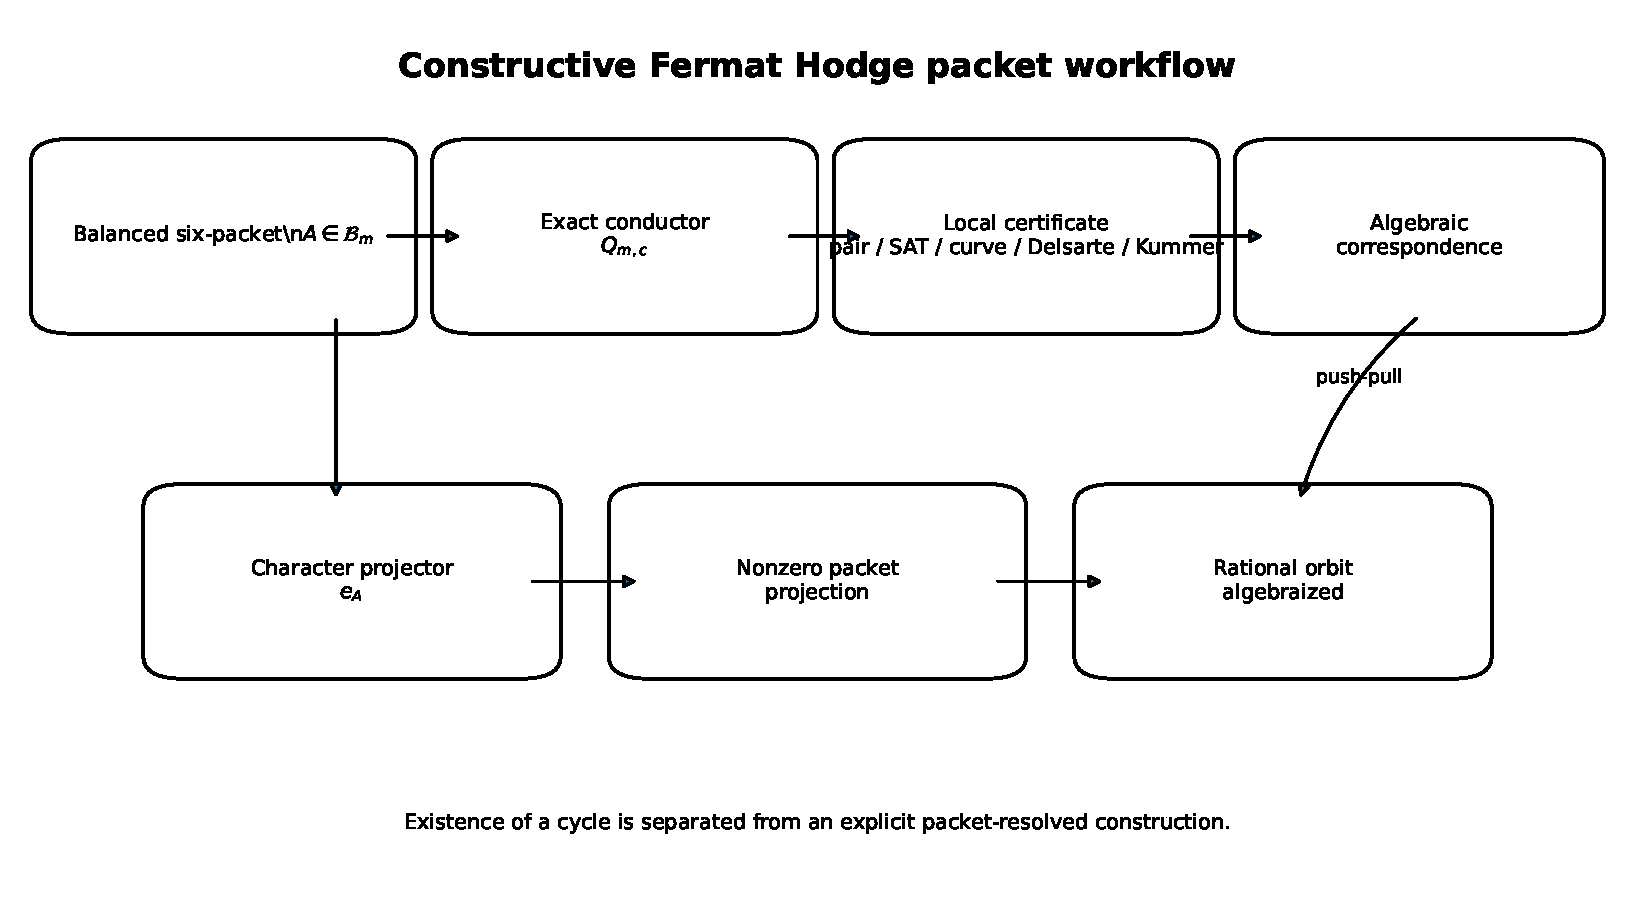
\includegraphics[width=0.84\textwidth]{33_fermat_packet_pipeline.pdf}
\vfill
{\small A theorem--proof monograph separating general Hodge infrastructure, Fermat packet classification, and explicit algebraic correspondence construction.\par}
{\small The general rational Hodge conjecture is not claimed as proved. The all-degree Fermat existence theorem is recorded as prior published work; the constructive packet program is the central contribution.\par}
\vspace{0.13in}
{\small August 2026\par}
\end{titlepage}
\hypersetup{pageanchor=true}

\chapter*{Abstract}
\addcontentsline{toc}{chapter}{Abstract}
This complete edition develops a projector-resolved Hodge calculus and then specializes it to the constructive geometry of Fermat fourfolds. The general infrastructure includes primitive Lefschetz reduction, the master Hodge obstruction projector, positive algebraic-cycle frames, exact polyphase assembly, finite saturation, support verification, divisor-lowering transfers, Adams degree projectors, and nonlinear Dolbeault obstruction packets. The Fermat specialization introduces the exact balanced-packet equation, conductor descent, M\"obius exact-conductor projectors, saturated packet identities, dual charges, curve and Delsarte channels, an explicit degree-33 Klein--Delsarte closure, infinite packet towers, odd prime-power classification, weighted dyadic refinement, an all-degree dyadic uniqueness theorem, CRT--Kummer phase grammar, K23 pair--triple factorization, and an imaginary CM half-twist selector. The dyadic theorem identifies the balanced defect lattice with integer total variation on a trivalent tree and proves that a single four-star orbit is the only obstruction to SAT(2); that orbit is uniformly SAT(3). The finite verification program includes the original eighteen Hodge checks, exact degree-33 and conductor checks, odd prime-power audits, 89,478,480 dyadic coefficient identities, exact dyadic packet enumeration through degree 128, balanced-packet enumeration through degree 100, and 364 exact K23 CM-type certificates.

The final constructive target is an explicit rank-one Chow correspondence from a lower Fermat-curve CM factor to the K23 weight-one packet. The monograph carefully separates finite symbolic closure, correspondence-level proofs, published existence claims, and unresolved constructive maps.

\begin{claimboundary}
The general rational Hodge conjecture remains open. Kang states a generalized-Hodge theorem for Fermat varieties of dimensions three and four in arbitrary degree \cite{KangFermat}; that prior existence theorem is not presented as new here. The new constructive program seeks explicit packet-resolved cycles and correspondences. Numerical and finite exact checks do not replace universal Chow-level correspondence proofs.
\end{claimboundary}

\chapter*{Executive map}
\addcontentsline{toc}{chapter}{Executive map}
The working grammar is
\[
\text{seed}\to\text{address}\to\text{operate}\to\text{project}
\to\text{transfer}\to\text{refine}\to\text{constrain}
\to\text{complete}\to\text{reconstruct}.
\]
For the Hodge problem, the seed is a rational cohomology class. Its first address is Hodge type, followed by Lefschetz depth, algebraic support, cycle degree, symmetry character, and arithmetic phase. Analysis is performed by cycle classes or algebraic correspondences. Refinement replaces one parent channel by complete children while preserving the total positive frame operator. The unresolved class is the intersection of the kernels of all available analysis channels.

\begin{center}
\begin{tabular}{p{0.23\textwidth}p{0.23\textwidth}p{0.42\textwidth}}
\toprule
Layer & Main object & Exact question \\
\midrule
Hodge selection & $P_{\Hdg}^p$ & Is the rational $(p,p)$ packet nonzero? \\
Algebraic selection & $P_{\Alg}^p$ & Which directions are already generated by cycles? \\
Master obstruction & $\mathcal O_X^p=P_{\Hdg}^p-P_{\Alg}^p$ & Does any Hodge direction survive all algebraic channels? \\
Cycle frame & $S_D=C_DC_D^*$ & Does a finite cycle family span the Hodge packet? \\
Polyphase refinement & $S_{M,r}=\sum_j S_{LM,r+jM}$ & Can separate geometric methods solve separate children? \\
Correspondence transfer & $T=\sum_rB_rA_r$ & Is lowering to divisor degree and returning invertible? \\
Analytic obstruction & $\Phi_A$ & Does the finite nonlinear obstruction packet vanish? \\
\bottomrule
\end{tabular}
\end{center}

{\small\setlength{\parskip}{0pt}\tableofcontents}

\mainmatter

\addcontentsline{toc}{part}{Part I. The conjecture as a projector problem}

\chapter{The rational Hodge target}
\section{Statement and status}
Let $X$ be a smooth projective complex variety. For each codimension $p$, define
\[
\Hdg^p(X)=H^{2p}(X,\Q)\cap H^{p,p}(X)
\]
and
\[
\Alg^p(X)=\im\bigl(\CH^p(X)_{\Q}\xrightarrow{\cl}H^{2p}(X,\Q)\bigr).
\]
Every algebraic cycle class has type $(p,p)$, so $\Alg^p(X)\subseteq\Hdg^p(X)$. The rational Hodge conjecture asserts equality for every smooth projective $X$ and every $p$ \cite{ClayHodge,VoisinHodge}.

Choose a polarization-compatible positive inner product on $H^{2p}(X,\R)$ and let $P_{\Hdg}^p$ and $P_{\Alg}^p$ denote orthogonal projectors. Since the algebraic space is nested in the Hodge space,
\[
P_{\Hdg}^pP_{\Alg}^p=P_{\Alg}^p.
\]

\begin{proposition}[Master obstruction projector]
The operator
\[
\mathcal O_X^p=P_{\Hdg}^p-P_{\Alg}^p
\]
is the orthogonal projector onto $\Hdg^p(X)\cap\Alg^p(X)^\perp$. Therefore
\[
\mathcal O_X^p=0
\quad\Longleftrightarrow\quad
\Hdg^p(X)=\Alg^p(X).
\]
\end{proposition}
\begin{proof}
For nested orthogonal projectors $Q\le P$, the difference $P-Q$ is self-adjoint and
\[
(P-Q)^2=P-PQ-QP+Q=P-Q.
\]
Its range is $\im P\cap(\im Q)^\perp$.
\end{proof}

\begin{figure}[htbp]
\centering
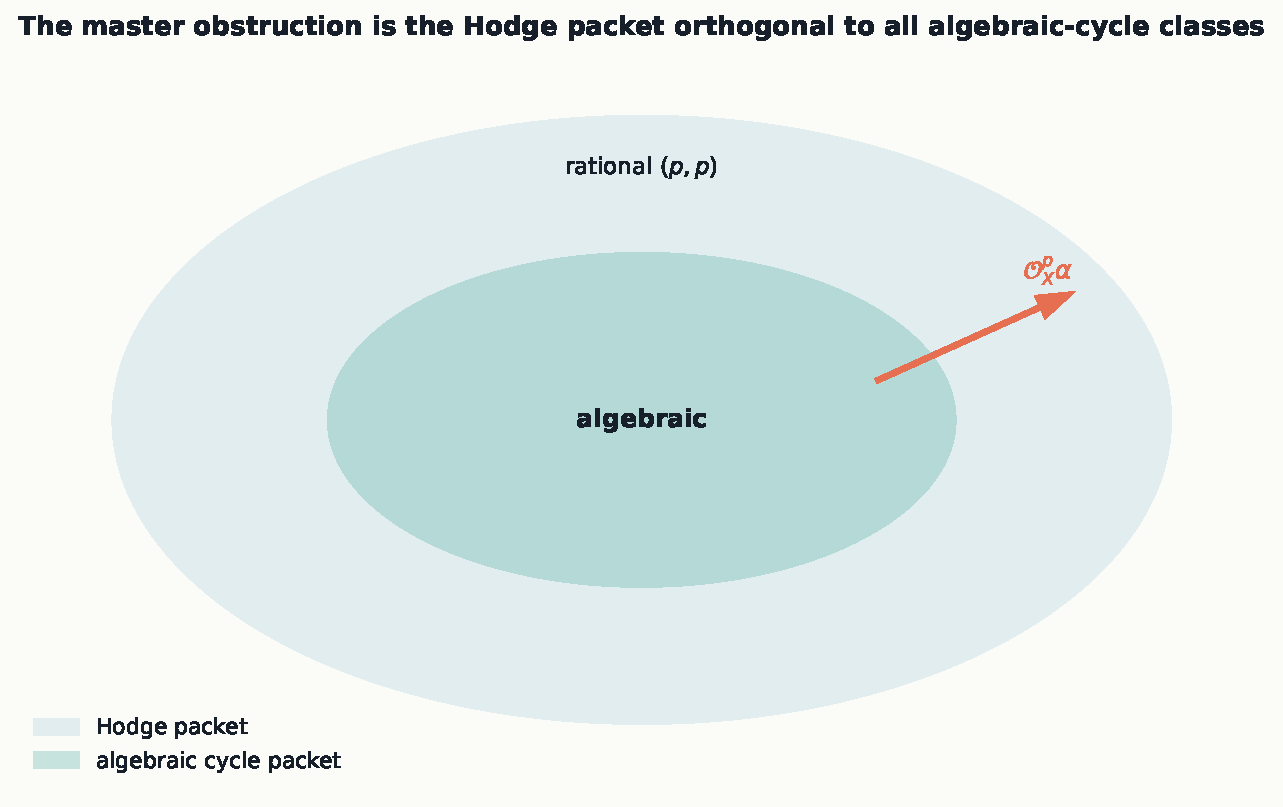
\includegraphics[width=0.82\textwidth]{04_master_obstruction_projector.pdf}
\caption{The master obstruction packet is the rational Hodge subspace not yet covered by algebraic cycle classes.}
\end{figure}

\section{Why dimension four is the first focused target}
The first general unresolved middle case occurs for primitive degree-four cohomology on a smooth projective fourfold. The Hodge diamond highlights the central packet.

\begin{figure}[htbp]
\centering
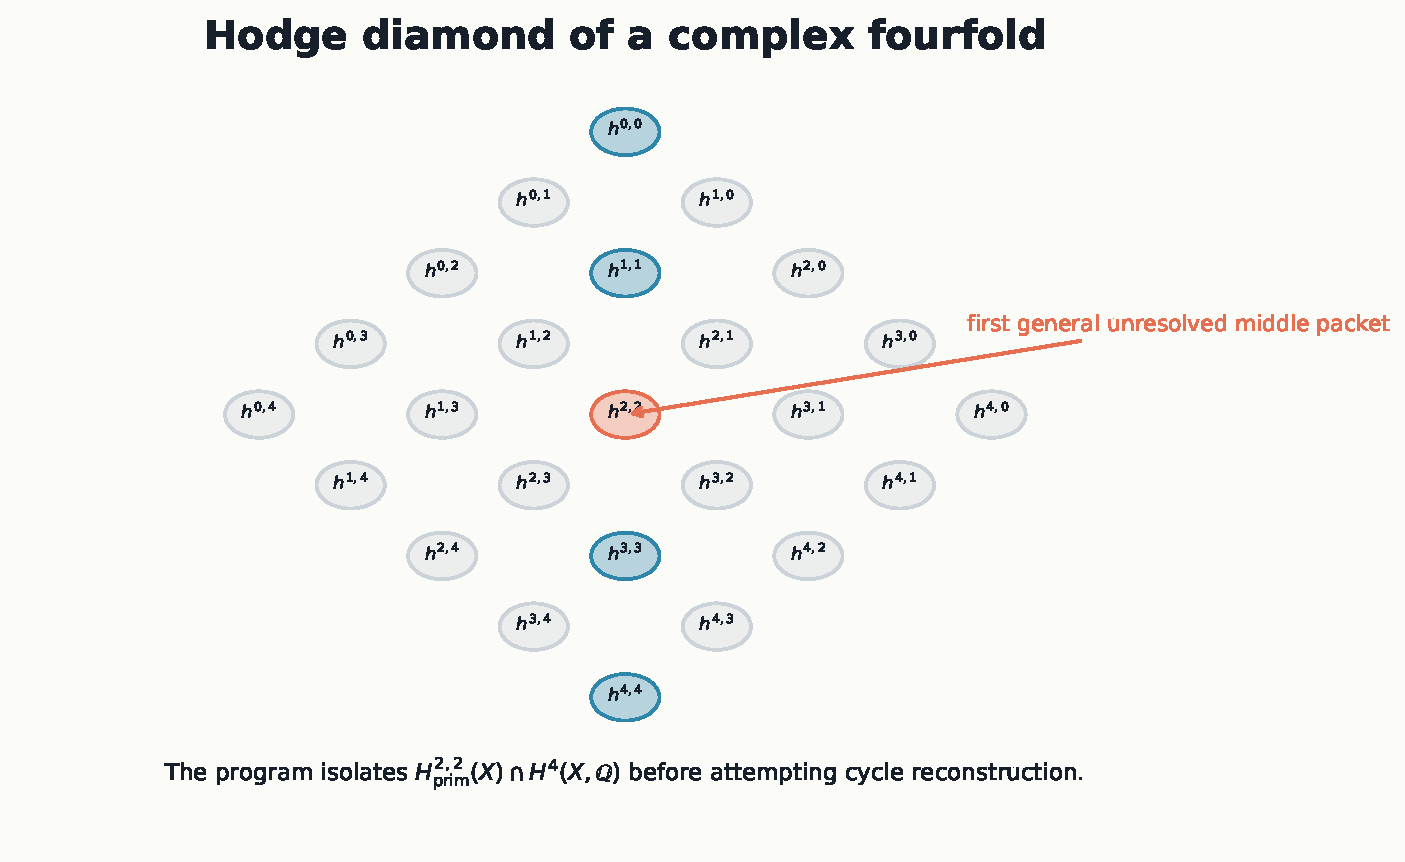
\includegraphics[width=0.68\textwidth]{02_fourfold_hodge_diamond.pdf}
\caption{The primitive rational $(2,2)$ packet in $H^4$ is the first general target retained by the program.}
\end{figure}

\chapter{Primitive and coniveau reductions}
\section{Lefschetz packet decomposition}
Let $h\in H^2(X,\Q)$ be the class of an ample divisor and let $L(\alpha)=h\smile\alpha$. Hard Lefschetz and primitive decomposition yield
\[
H^{2p}(X,\Q)=\bigoplus_{r\ge0}L^rH_{\mathrm{prim}}^{2p-2r}(X,\Q).
\]
The decomposition respects Hodge type.

\begin{theorem}[Primitive reduction]
If every primitive rational Hodge class is algebraic, then every rational Hodge class is algebraic.
\end{theorem}
\begin{proof}
Write $\alpha=\sum_rL^r\alpha_r$ with each $\alpha_r$ primitive and of Hodge type. The class $h$ is algebraic. If $\alpha_r$ is algebraic, then $L^r\alpha_r=h^r\smile\alpha_r$ is algebraic. Summing gives an algebraic representative of $\alpha$.
\end{proof}

For a fourfold and $p=2$,
\[
\alpha=L\beta+\alpha_{\mathrm{prim}},
\qquad
\beta\in H^{1,1}(X)\cap H^2(X,\Q).
\]
The Lefschetz $(1,1)$ theorem makes $\beta$ algebraic. Only $\alpha_{\mathrm{prim}}$ remains.

\begin{figure}[htbp]
\centering
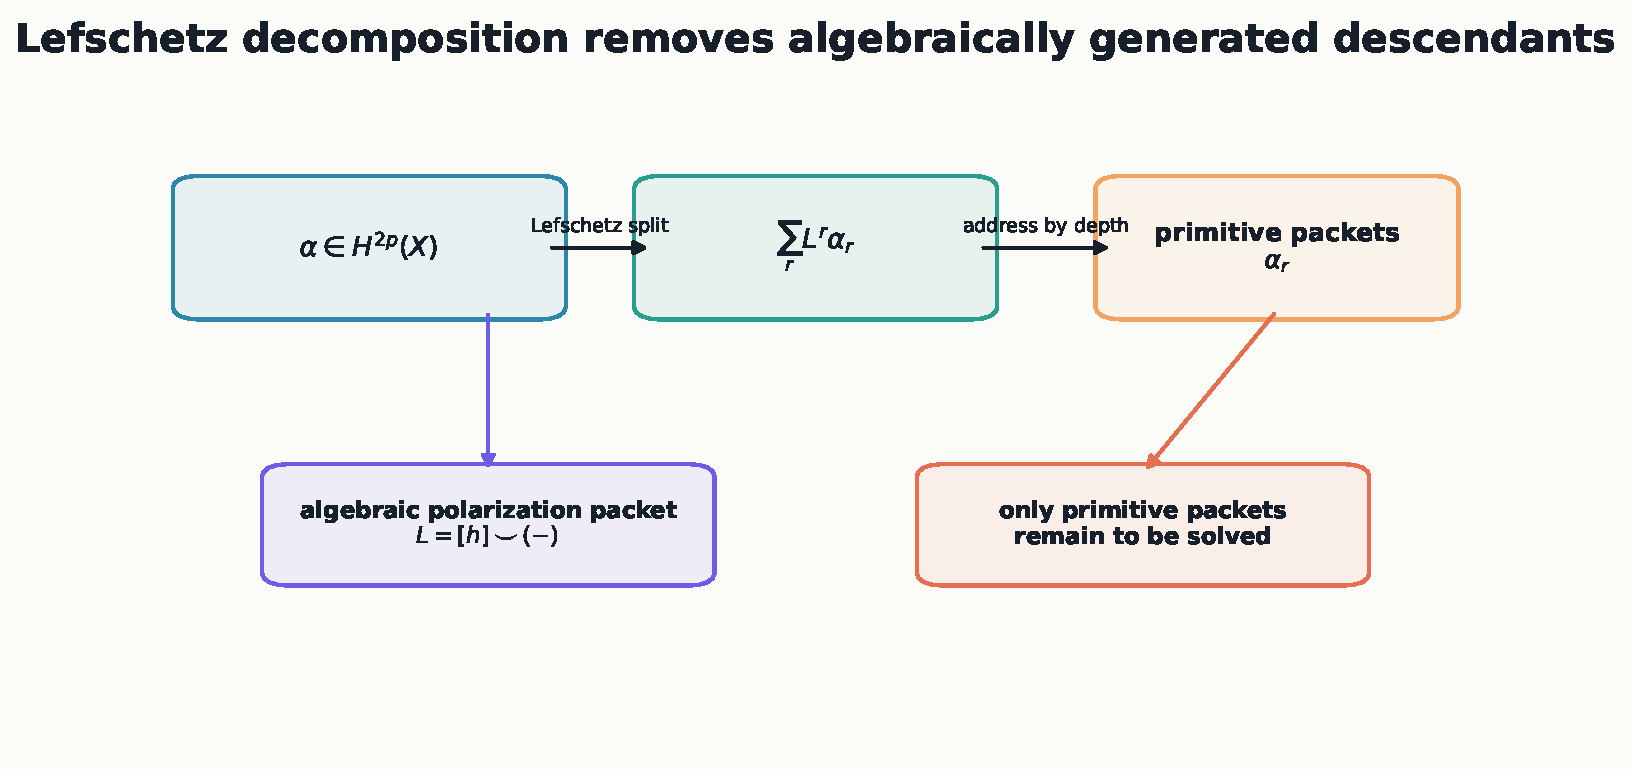
\includegraphics[width=0.82\textwidth]{03_lefschetz_primitive_reduction.pdf}
\caption{Algebraic powers of the polarization remove all Lefschetz descendants, leaving primitive packets.}
\end{figure}

\section{Support localization and coniveau}
Let $N^pH^{2p}(X,\Q)$ be the geometric coniveau-$p$ subspace. In degree $2p$, purity forces support contributions of codimension $p$ to be generated by fundamental classes of codimension-$p$ components.

\begin{theorem}[Degree-$2p$ coniveau identification]
For smooth projective $X$,
\[
N^pH^{2p}(X,\Q)=\Alg^p(X).
\]
\end{theorem}
\begin{proof}[Proof sketch]
The inclusion from right to left is immediate because a codimension-$p$ cycle is supported on its underlying algebraic set. Conversely, a class in coniveau $p$ is in the image of cohomology with supports in an algebraic subset $Z$ of codimension at least $p$. Contributions from components of codimension greater than $p$ vanish in degree $2p$. Purity identifies the degree-$2p$ supported contribution of each codimension-$p$ irreducible component with its fundamental class. Resolution and additivity reduce a general $Z$ to these components.
\end{proof}

Thus the conjecture is equivalently the support statement
\[
\Hdg^p(X)\subseteq N^pH^{2p}(X,\Q).
\]

\begin{figure}[htbp]
\centering
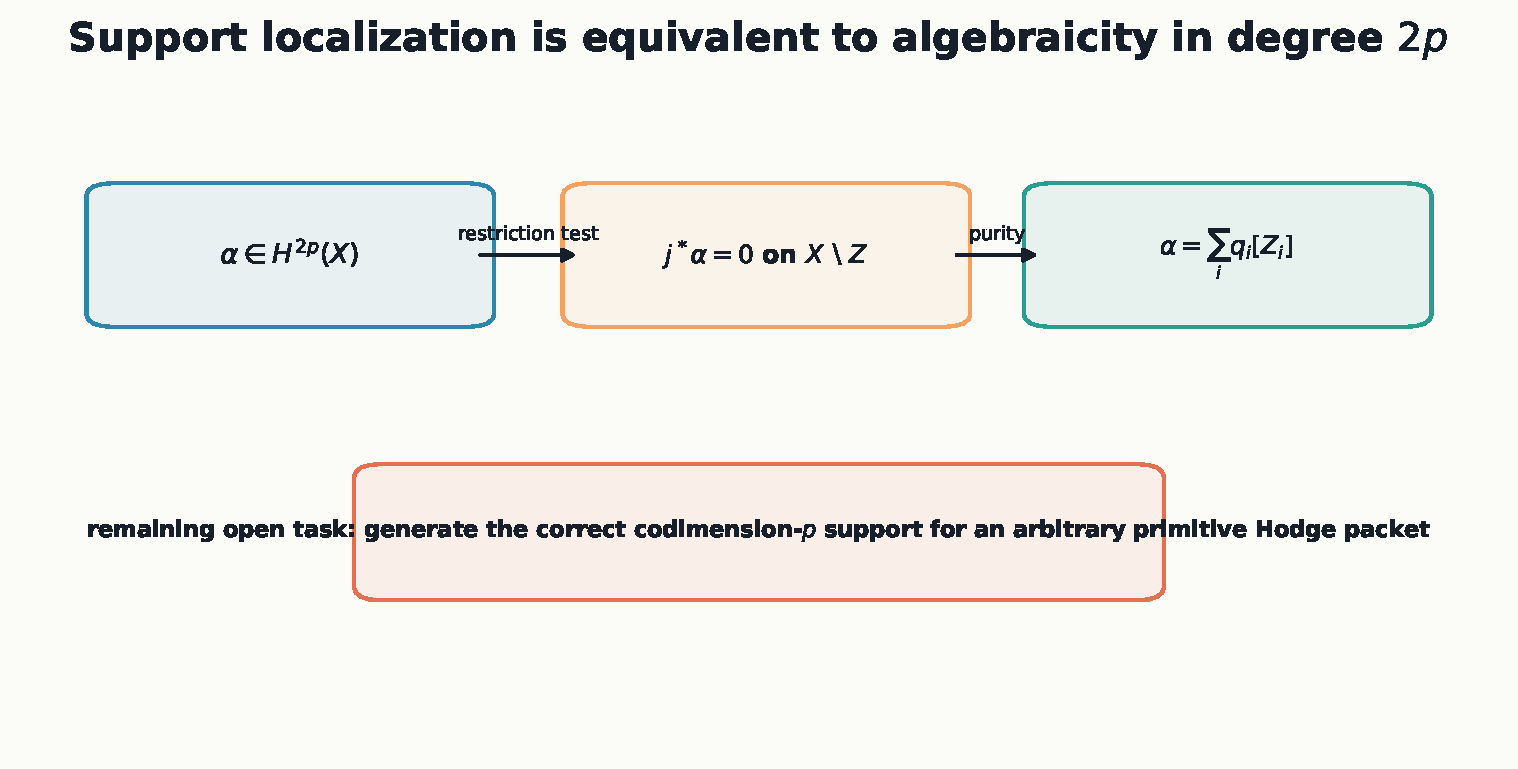
\includegraphics[width=0.84\textwidth]{05_support_localization_pipeline.pdf}
\caption{A verified codimension-$p$ support turns the Hodge class into a finite rational combination of support components.}
\end{figure}

\addcontentsline{toc}{part}{Part II. Algebraic cycle frames and exact polyphase refinement}

\chapter{Positive cycle-frame calculus}
\section{Analysis and synthesis}
Fix a finite family of rational algebraic cycle classes
\[
c_1,\ldots,c_N\in H^{2p}(X,\Q).
\]
Let $V\subseteq H^{2p}(X,\R)$ be the Hodge packet under study. Define
\[
C:\R^N\to H^{2p}(X,\R),
\qquad Ce_j=c_j,
\]
and the positive frame operator
\[
S=CC^*=\sum_{j=1}^N|c_j\rangle\langle c_j|.
\]

\begin{theorem}[Finite positive cycle-frame certificate]
Let $A=\Span_{\R}\{c_1,\ldots,c_N\}$. Then
\[
\im S=A,
\qquad
\ker S=A^\perp.
\]
The selected cycles span $V$ if and only if $S|_V$ is positive definite.
\end{theorem}
\begin{proof}
The equality $\im(CC^*)=\im C$ is standard. Moreover
\[
\langle v,Sv\rangle=\|C^*v\|^2=\sum_j|\langle c_j,v\rangle|^2.
\]
This vanishes exactly when $v$ is orthogonal to every cycle class.
\end{proof}

If $H$ is a matrix whose columns form an orthonormal basis of $V$, the finite Gram certificate is
\[
G=H^*SH.
\]
Then $A\supseteq V$ if and only if $\lambda_{\min}(G)>0$.

\begin{figure}[htbp]
\centering
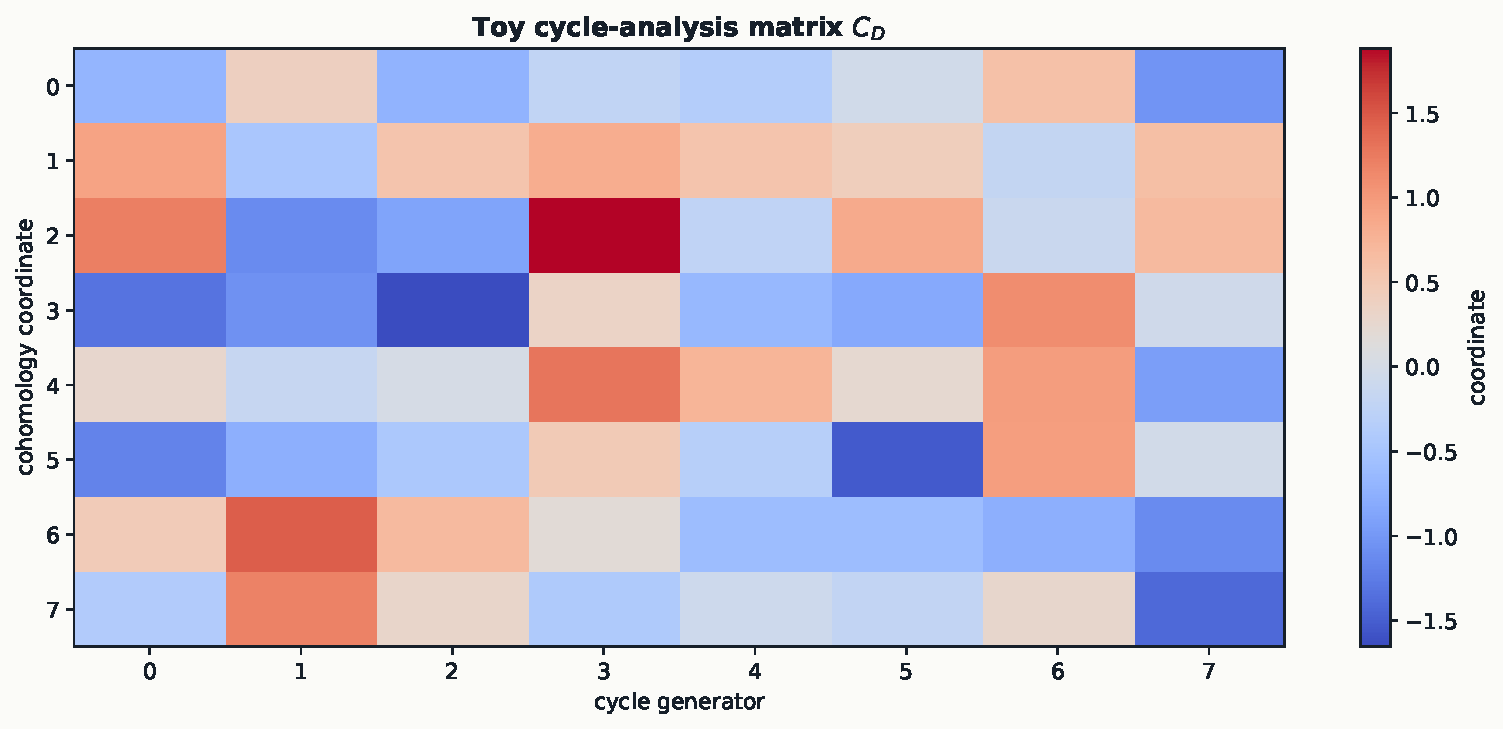
\includegraphics[width=0.82\textwidth]{06_cycle_analysis_matrix.pdf}
\caption{A finite cycle-analysis matrix records cohomology coordinates of candidate algebraic cycles.}
\end{figure}

\begin{figure}[htbp]
\centering
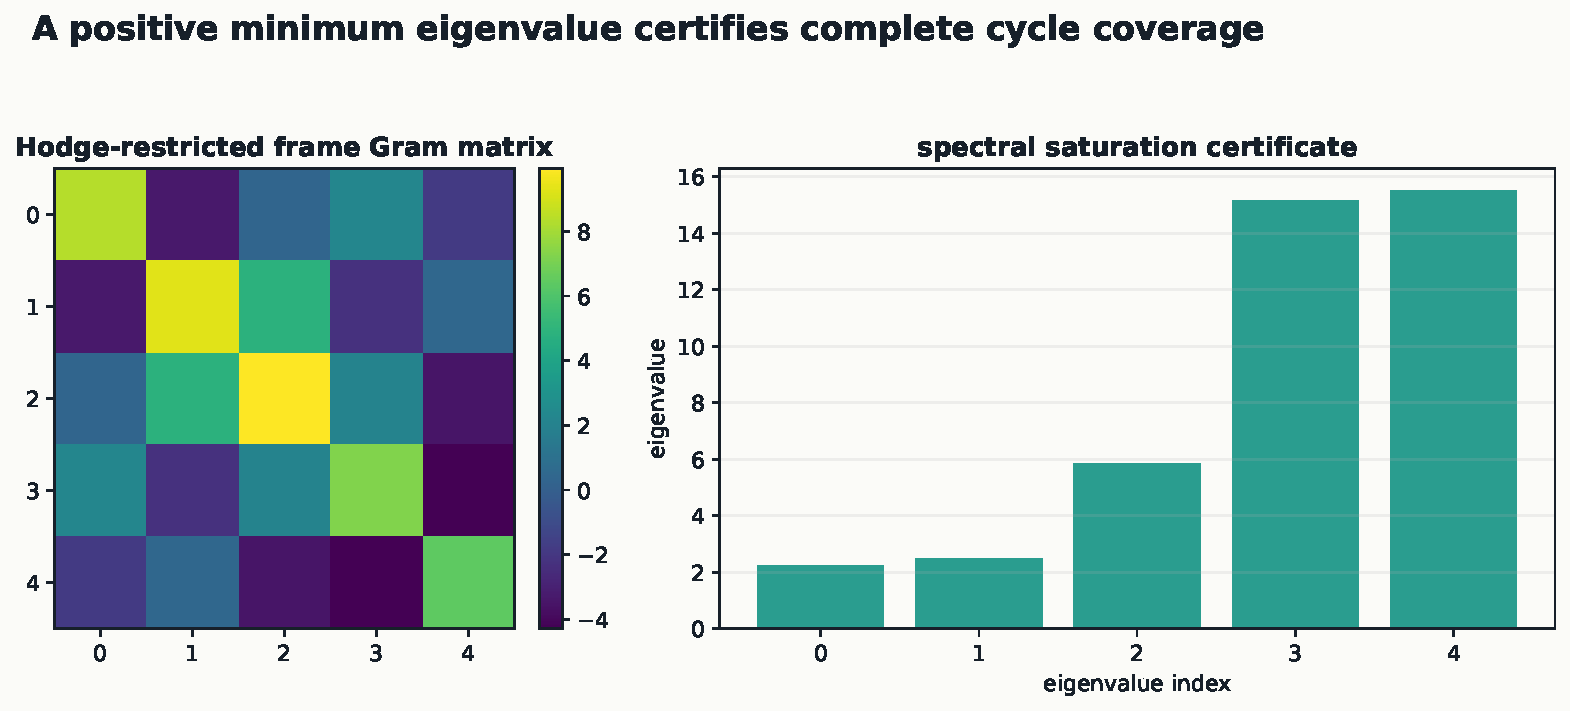
\includegraphics[width=0.9\textwidth]{07_cycle_frame_spectrum.pdf}
\caption{The Hodge-restricted Gram spectrum gives a finite spectral saturation certificate.}
\end{figure}

The orthogonal synthesis of a class $\alpha$ from the cycle span is
\[
P_A\alpha=S S^\dagger\alpha.
\]
If $\alpha\in A$, this is exact.

\begin{figure}[htbp]
\centering
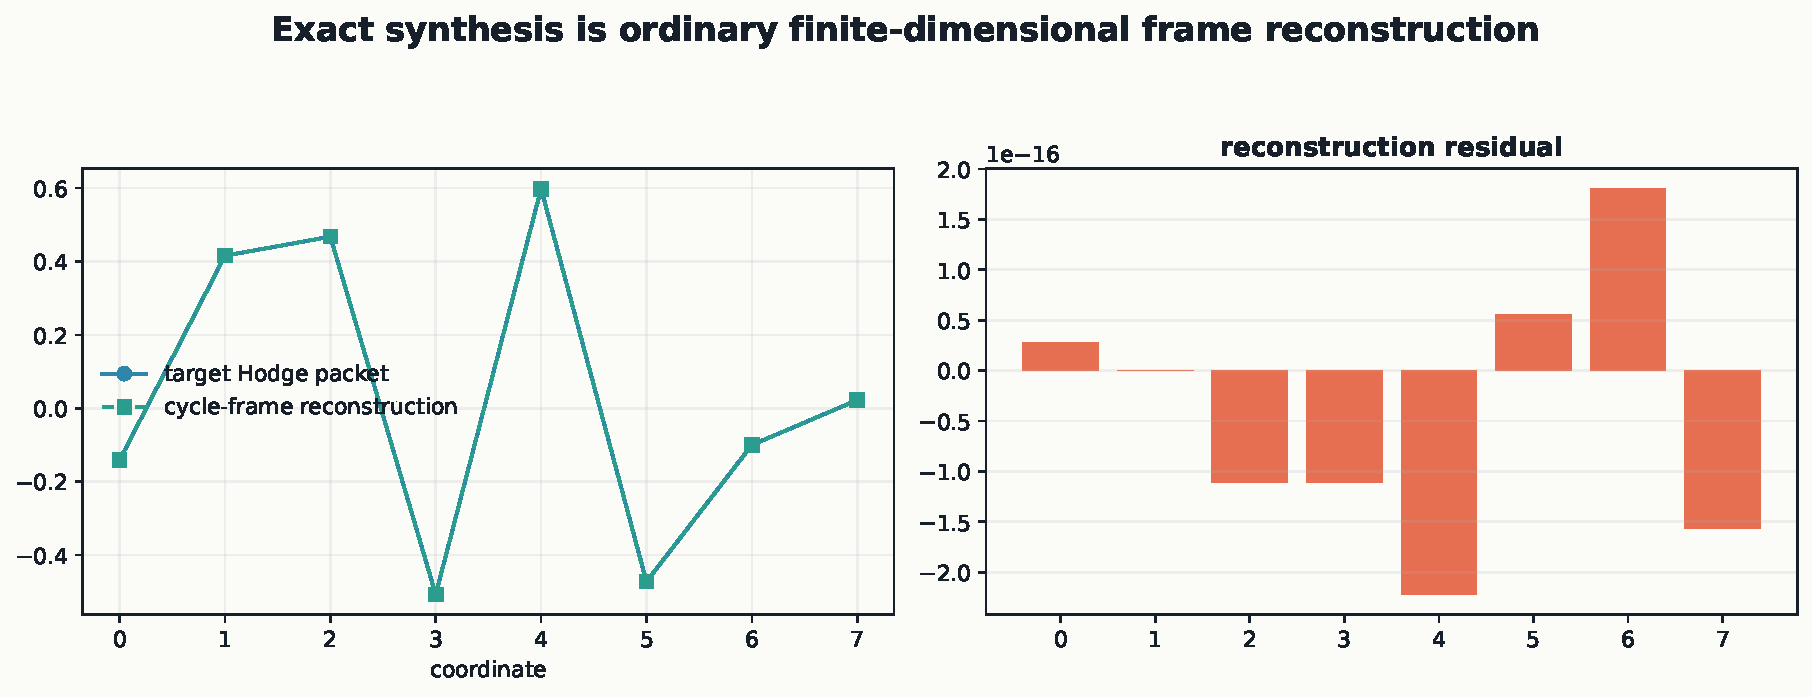
\includegraphics[width=0.88\textwidth]{08_cycle_frame_reconstruction.pdf}
\caption{Finite-dimensional frame synthesis reconstructs the class whenever it lies in the algebraic span.}
\end{figure}

\section{Packet assembly without false orthogonality}
Partition the cycle indices into packets $I_\lambda$. Define
\[
S_\lambda=\sum_{j\in I_\lambda}|c_j\rangle\langle c_j|.
\]
Then
\[
S=\sum_\lambda S_\lambda.
\]
No orthogonality of the child spans is assumed.

\begin{theorem}[Positive child-kernel intersection]
For any subspace $V$,
\[
\ker(S|_V)=\bigcap_\lambda\ker(S_\lambda|_V).
\]
\end{theorem}
\begin{proof}
If $Sv=0$, positivity gives
\[
0=\langle v,Sv\rangle=\sum_\lambda\langle v,S_\lambda v\rangle.
\]
Each nonnegative summand vanishes, which implies $S_\lambda v=0$. The converse is immediate.
\end{proof}

\begin{figure}[htbp]
\centering
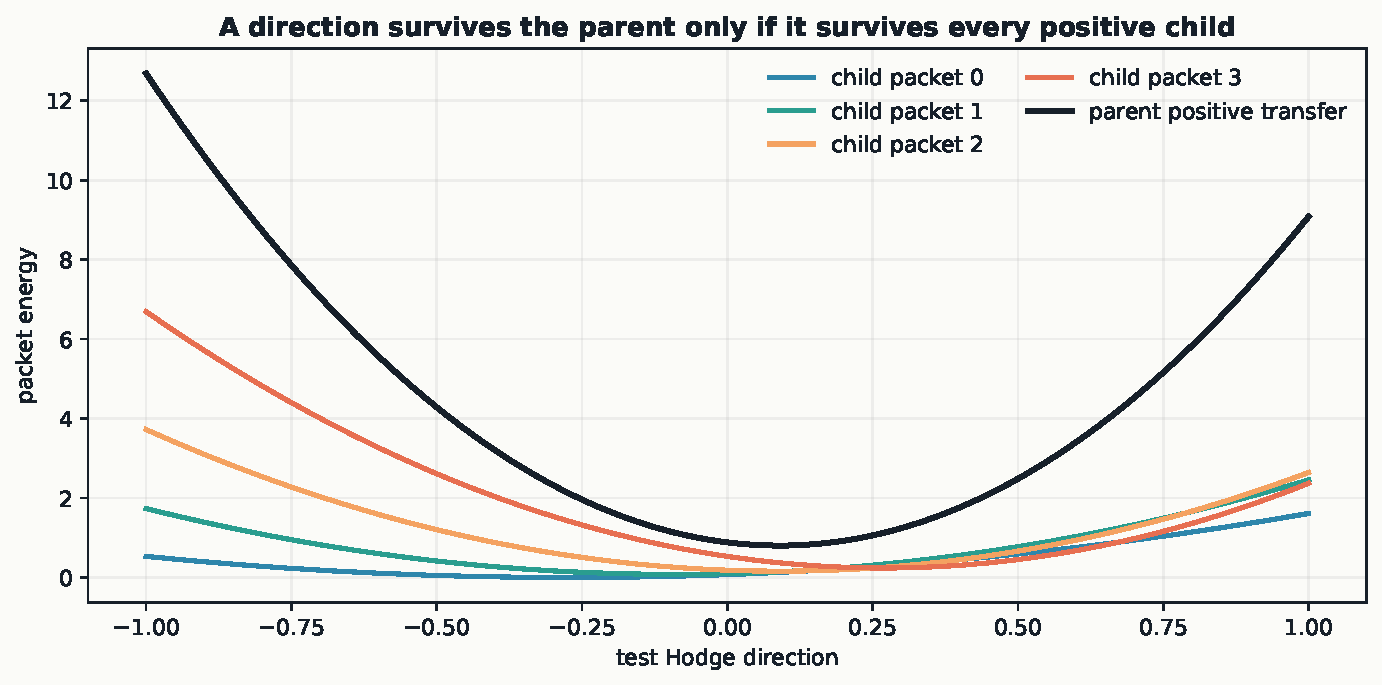
\includegraphics[width=0.84\textwidth]{11_child_kernel_intersection.pdf}
\caption{A Hodge direction survives the parent obstruction only when every positive child channel misses it.}
\end{figure}

\chapter{Degree-residue polyphase refinement}
\section{Exact parent-child frame law}
Fix a projective embedding and assign each cycle its degree. For modulus $M$, define the residue packet
\[
I_{M,r}=\{j:\deg Z_j\equiv r\pmod M\},
\qquad
S_{M,r}=\sum_{j\in I_{M,r}}|c_j\rangle\langle c_j|.
\]

\begin{theorem}[Exact degree polyphase refinement]
For every positive integer $L$,
\[
S_{M,r}=\sum_{\ell=0}^{L-1}S_{LM,r+\ell M}.
\]
\end{theorem}
\begin{proof}
The congruence class $r$ modulo $M$ is the disjoint union of the classes $r+\ell M$ modulo $LM$. The rank-one frame terms are partitioned accordingly.
\end{proof}

\begin{figure}[htbp]
\centering
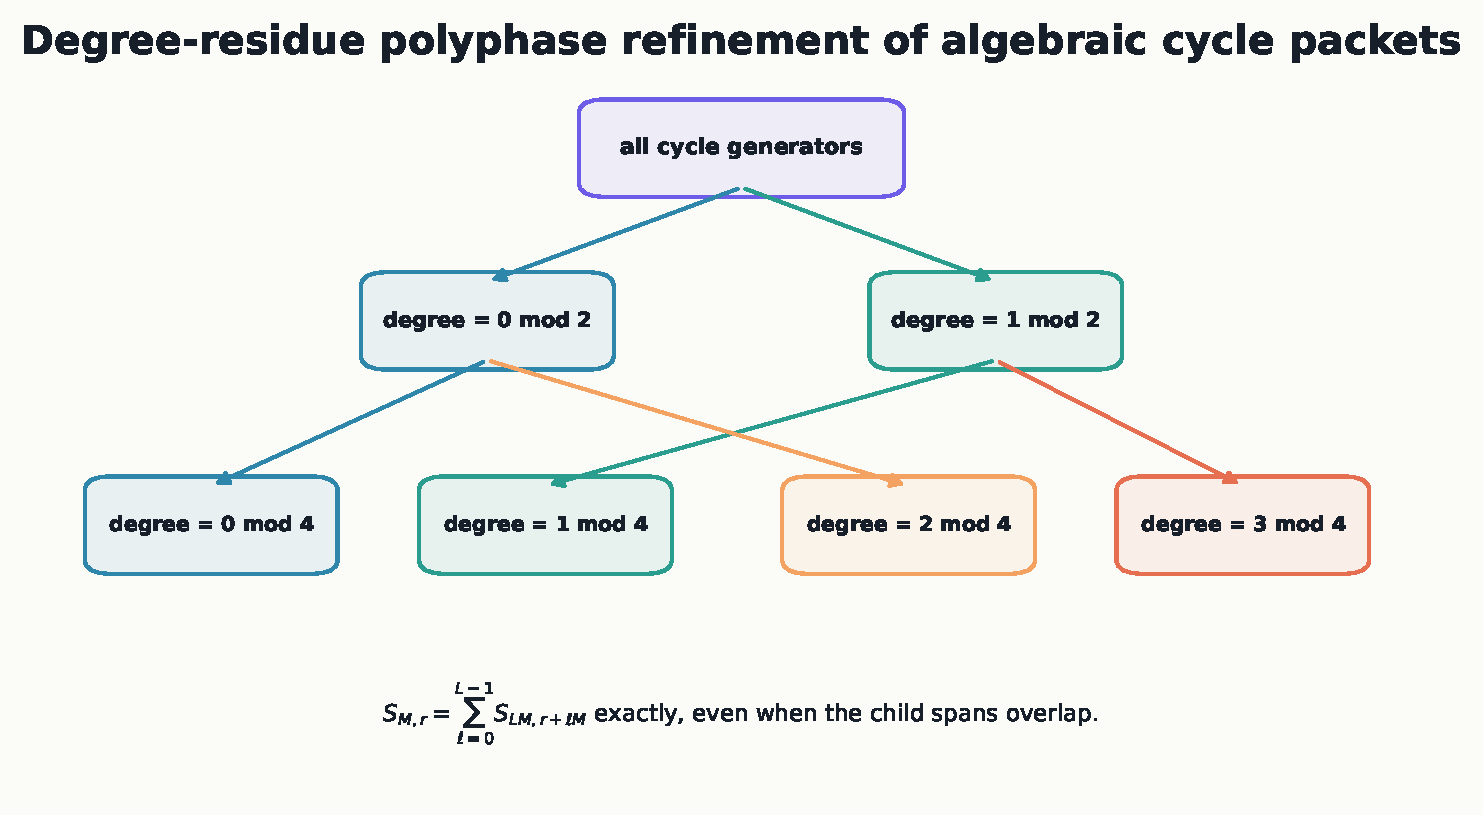
\includegraphics[width=0.82\textwidth]{09_degree_polyphase_tree.pdf}
\caption{Degree addresses refine from modulo $2$ to modulo $4$ while the total cycle frame remains unchanged.}
\end{figure}

\begin{figure}[htbp]
\centering
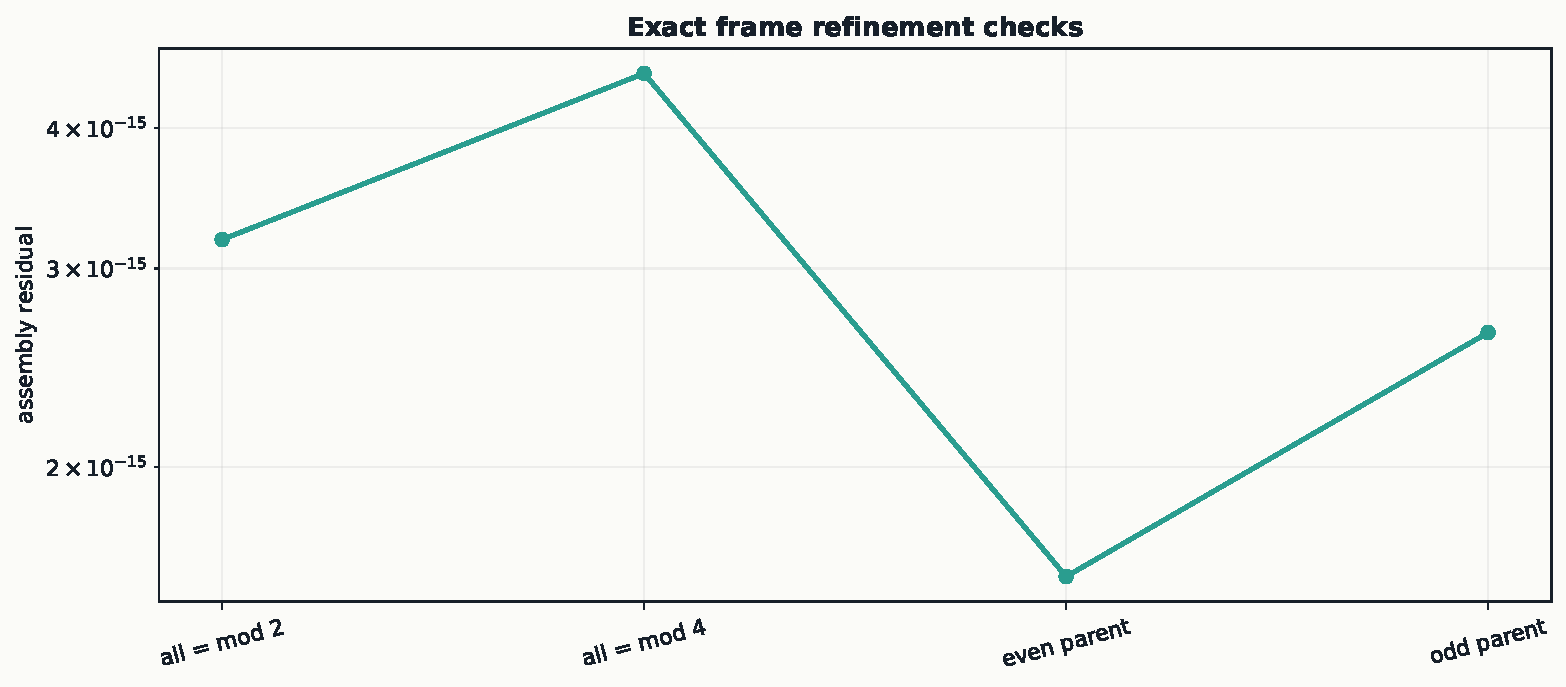
\includegraphics[width=0.76\textwidth]{10_polyphase_assembly_residuals.pdf}
\caption{Numerical certificates of exact parent-child frame assembly in the reproducible toy model.}
\end{figure}

\section{Multiaxial packet addresses}
Degree residue is only one address. A refined cycle packet may be labeled by
\[
\lambda=(r_{\mathrm{Lef}},r_{\deg},\chi_{\mathrm{mon}},s_{\mathrm{supp}},\nu_{\mathrm{Frob}}).
\]
The entries record Lefschetz depth, degree residue, monodromy or symmetry type, support stratum, and arithmetic phase. The total positive frame remains the sum of all leaves. This allows independent methods to solve different geometric sectors before exact synthesis.

\chapter{Finite saturation and exact rational closure}
For each degree cutoff $D$, let $A_D^p(X)$ be the rational span of codimension-$p$ cycle classes of degree at most $D$. Then
\[
A_1^p\subseteq A_2^p\subseteq\cdots\subseteq H^{2p}(X,\Q).
\]

\begin{theorem}[Finite stabilization]
There exists $D_0$ such that $A_D^p(X)=A_{D_0}^p(X)$ for every $D\ge D_0$.
\end{theorem}
\begin{proof}
The dimensions form a nondecreasing sequence of integers bounded by $\dim H^{2p}(X,\Q)$. Only finitely many strict increases are possible.
\end{proof}

\begin{corollary}[Approximation becomes exact]
Let $P_D$ be the orthogonal projector onto $A_D^p(X)\otimes\R$. For a rational class $\alpha$,
\[
\lim_{D\to\infty}\|(I-P_D)\alpha\|=0
\]
if and only if $\alpha\in A_D^p(X)$ for some finite $D$.
\end{corollary}
\begin{proof}
After stabilization, the residual is constant. A constant tail converging to zero is zero.
\end{proof}

Because the matrices and target vector can be chosen over $\Q$, real membership implies rational membership by row reduction over $\Q$.

\begin{figure}[htbp]
\centering
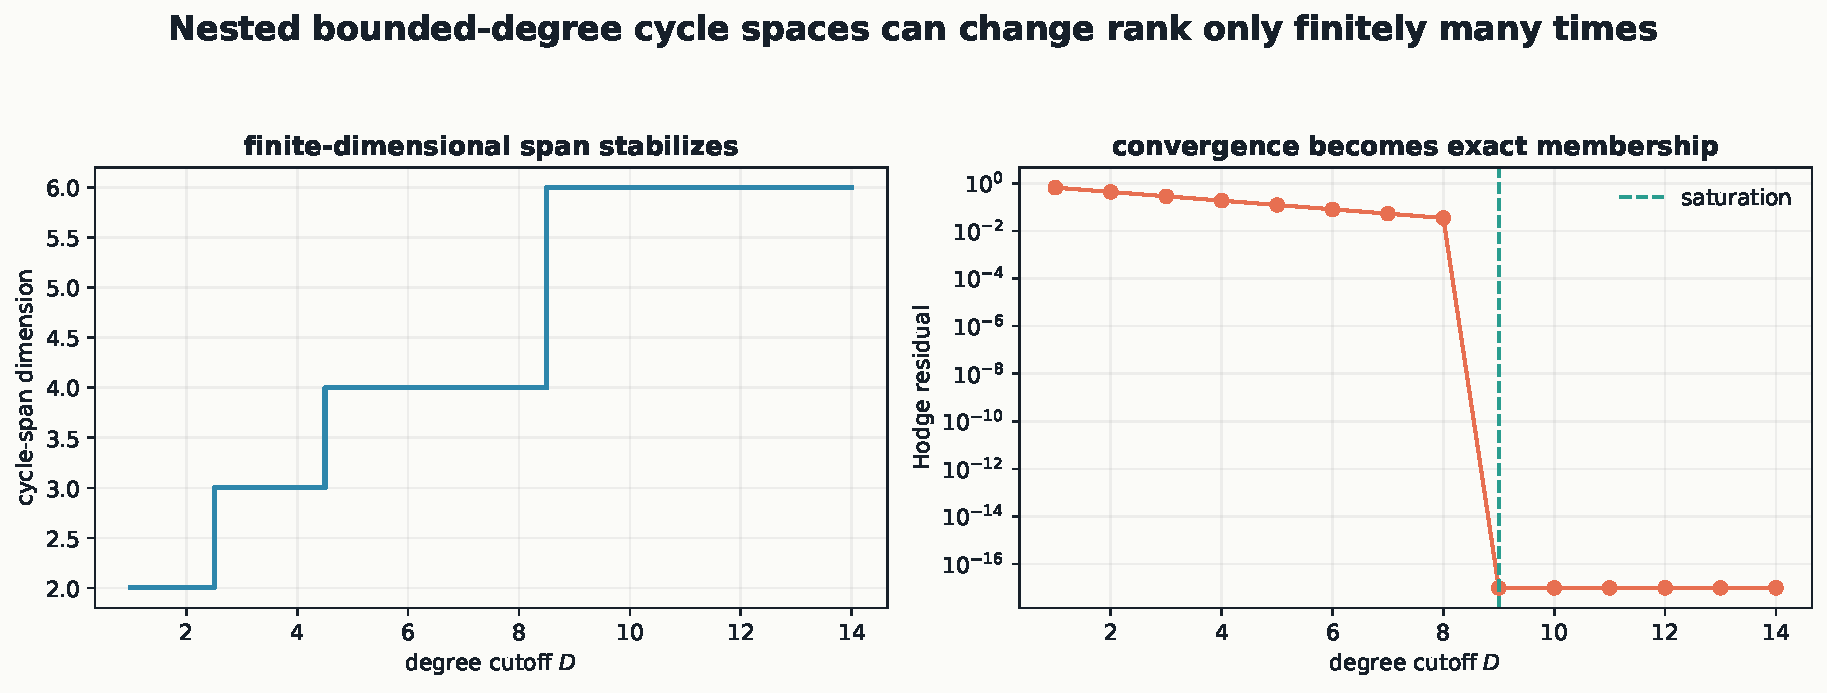
\includegraphics[width=0.9\textwidth]{12_finite_saturation.pdf}
\caption{The cycle span has a finite rank ceiling. Once the residual converges to zero, exact membership has already occurred at a finite stage.}
\end{figure}

\begin{resultbox}[Finite completion certificate]
If $H$ is a rational basis matrix of $\Hdg^p(X)$ and $C_D$ is the cycle matrix, then the Hodge conjecture for $(X,p)$ is equivalent to the existence of $D$ with
\[
\rank_{\Q} C_D=\rank_{\Q}[C_D\ H].
\]
Equivalently, the Hodge-restricted positive frame has positive minimum eigenvalue.
\end{resultbox}

\addcontentsline{toc}{part}{Part III. Support packets and correspondence reconstruction}

\chapter{Support verification and multiplicity recovery}
Let $Z\subseteq X$ be a closed algebraic subset and $j:X\setminus Z\hookrightarrow X$. The support exact sequence contains
\[
H_Z^{2p}(X,\Q)\longrightarrow H^{2p}(X,\Q)\xrightarrow{j^*}H^{2p}(X\setminus Z,\Q).
\]

\begin{theorem}[Exact support test]
A class $\alpha\in H^{2p}(X,\Q)$ is supported on $Z$ if and only if $j^*\alpha=0$.
\end{theorem}
\begin{proof}
This is exactness at the middle term.
\end{proof}

\begin{figure}[htbp]
\centering
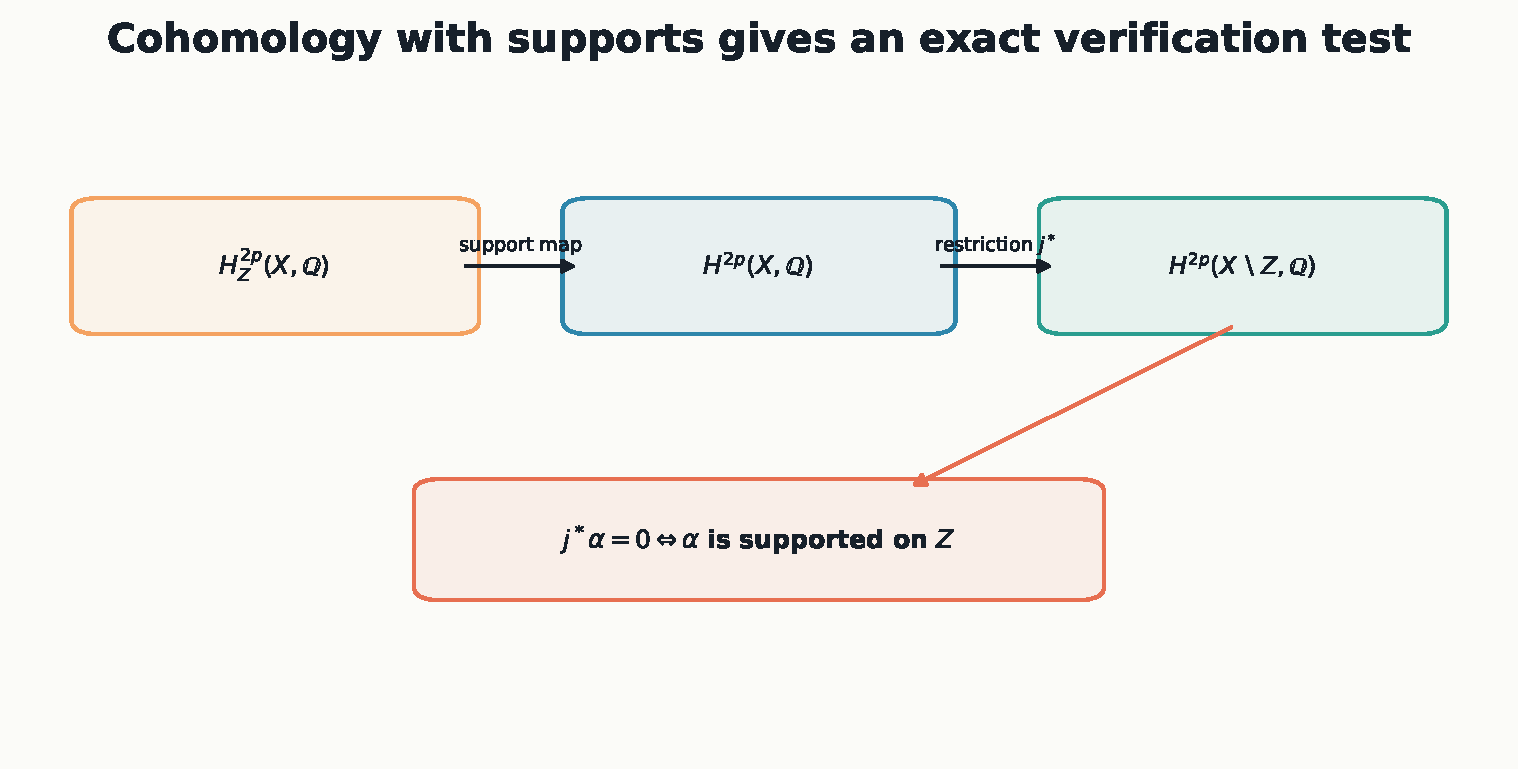
\includegraphics[width=0.82\textwidth]{14_support_exact_sequence.pdf}
\caption{Restriction to the complement provides an exact verification test for a proposed algebraic support.}
\end{figure}

Suppose the codimension-$p$ components are $Z_1,\ldots,Z_r$. Purity gives
\[
\alpha=\sum_{i=1}^r q_i[Z_i].
\]
Choose complementary test classes $\gamma_k$ and define
\[
M_{ki}=\int_X[Z_i]\smile\gamma_k,
\qquad
b_k=\int_X\alpha\smile\gamma_k.
\]
Then $Mq=b$. Removing dependent columns yields exact rational multiplicities.

\begin{figure}[htbp]
\centering
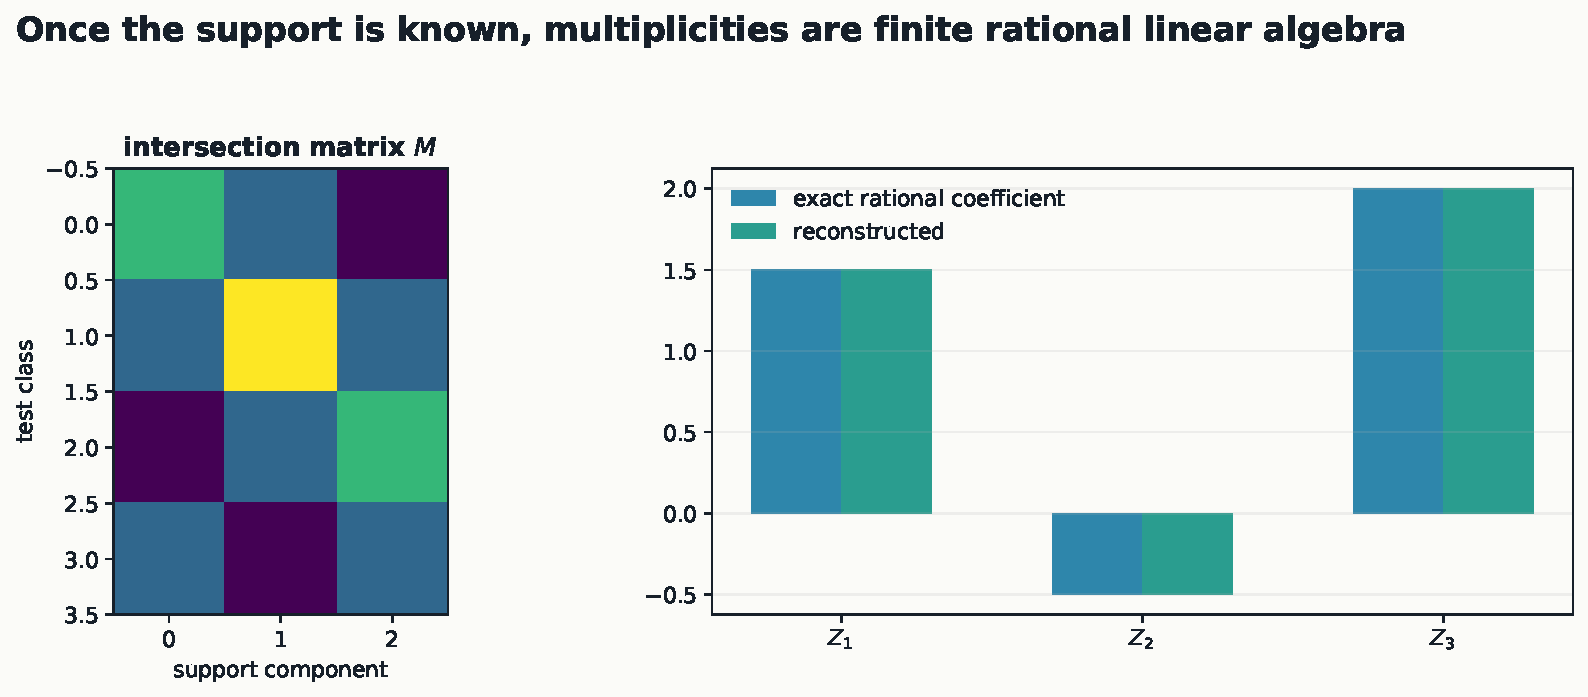
\includegraphics[width=0.9\textwidth]{13_support_multiplicity_reconstruction.pdf}
\caption{Once a support is verified, the cycle multiplicities are reconstructed by a finite rational linear system.}
\end{figure}

\chapter{Divisor-lowering correspondence channels}
\section{Degree bookkeeping}
Let $X$ have complex dimension $n$, let $V\subseteq H_{\mathrm{prim}}^{2p}(X,\Q)$ be a rational Hodge substructure, and let $Y_r$ be smooth projective. Choose correspondences
\[
\Gamma_r\in\CH^{n-p+1}(X\times Y_r)_{\Q},
\qquad
\Lambda_r\in\CH^{\dim Y_r+p-1}(Y_r\times X)_{\Q}.
\]
They induce
\[
A_r=(\Gamma_r)_*:V\to H^2(Y_r,\Q),
\qquad
B_r=(\Lambda_r)_*:H^2(Y_r,\Q)\to H^{2p}(X,\Q).
\]
Algebraic correspondences preserve rationality and shift Hodge type by the required bidegree.

\begin{theorem}[Invertible divisor-lowering transfer]
Suppose
\[
T=\sum_{r=1}^M B_rA_r
\]
preserves $V$ and is invertible on $V$. Then every rational Hodge class in $V$ is algebraic.
\end{theorem}
\begin{proof}
Let $\alpha\in V$ be of type $(p,p)$. Each $A_r\alpha$ is rational of type $(1,1)$ on $Y_r$, hence is the class of a rational divisor $D_r$ by the Lefschetz $(1,1)$ theorem. Therefore
\[
T\alpha=\sum_r(\Lambda_r)_*[D_r]
\]
is algebraic on $X$.

Let $\chi_T(t)=t^d+c_{d-1}t^{d-1}+\cdots+c_0$ be the characteristic polynomial on $V$. Invertibility means $c_0\ne0$. Cayley-Hamilton gives
\[
T^{-1}=-\frac{1}{c_0}\bigl(T^{d-1}+c_{d-1}T^{d-2}+\cdots+c_1I\bigr).
\]
Each power of $T$ is induced by compositions and rational sums of algebraic correspondences. Thus $T^{-1}$ preserves algebraic cycle classes. Hence $\alpha=T^{-1}(T\alpha)$ is algebraic.
\end{proof}

\begin{figure}[htbp]
\centering
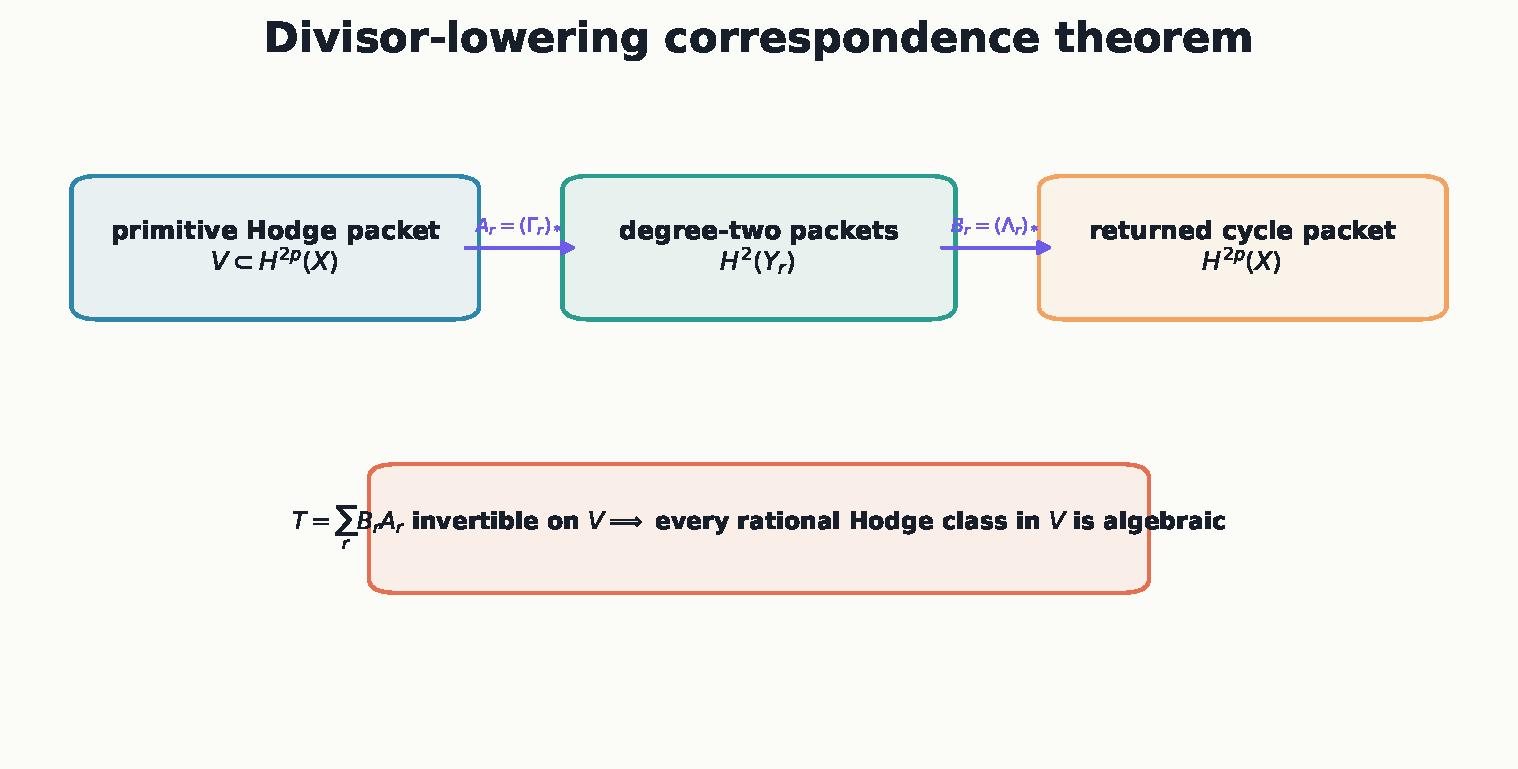
\includegraphics[width=0.86\textwidth]{15_divisor_lowering_transfer.pdf}
\caption{A primitive Hodge class is lowered to divisor degree, algebraized there, and returned through an invertible transfer.}
\end{figure}

\begin{figure}[htbp]
\centering
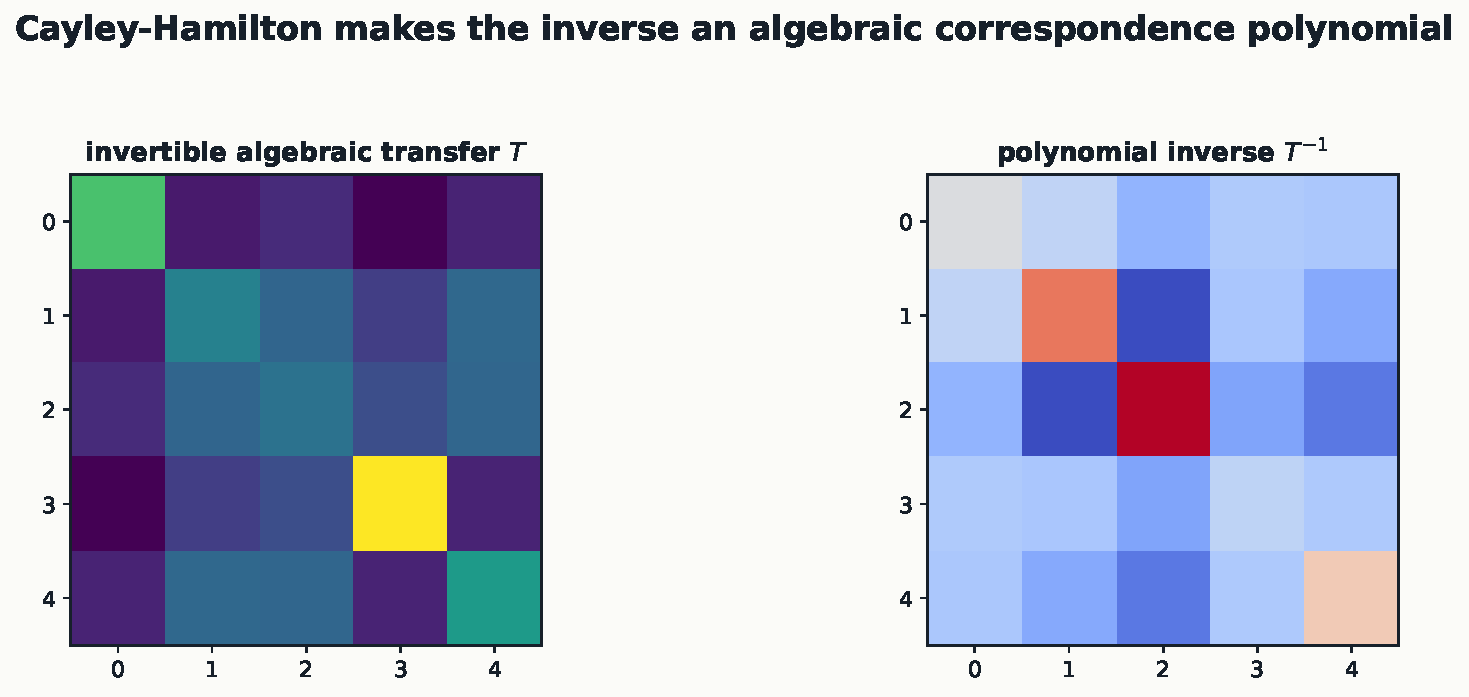
\includegraphics[width=0.82\textwidth]{18_cayley_hamilton_inverse.pdf}
\caption{The inverse transfer is a rational polynomial in the original algebraic correspondence operator.}
\end{figure}

\section{Positive multi-channel form}
Assume the polarized adjoint $A_r^\dagger$ is realized by an algebraic return correspondence $B_r$. This is an additional geometric hypothesis, not an automatic consequence in arbitrary settings. Then
\[
T=\sum_rA_r^\dagger A_r
\]
is positive and
\[
\langle v,Tv\rangle=\sum_r\|A_rv\|^2.
\]
Therefore
\[
\ker T=\bigcap_r\ker A_r.
\]
Joint injectivity of the lowering channels is enough.

\begin{figure}[htbp]
\centering
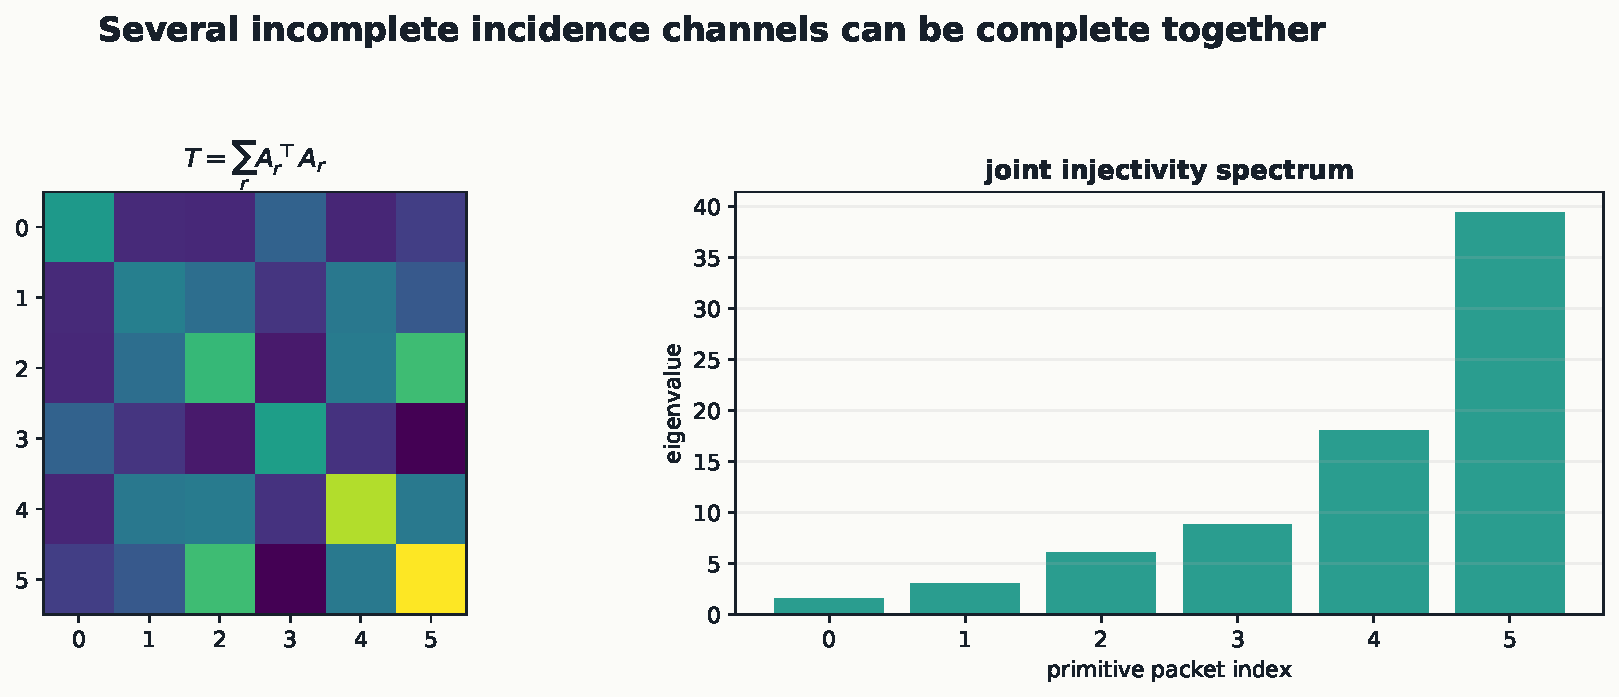
\includegraphics[width=0.88\textwidth]{16_positive_correspondence_frame.pdf}
\caption{Several incidence channels may be individually incomplete while their positive sum is invertible.}
\end{figure}

\begin{figure}[htbp]
\centering
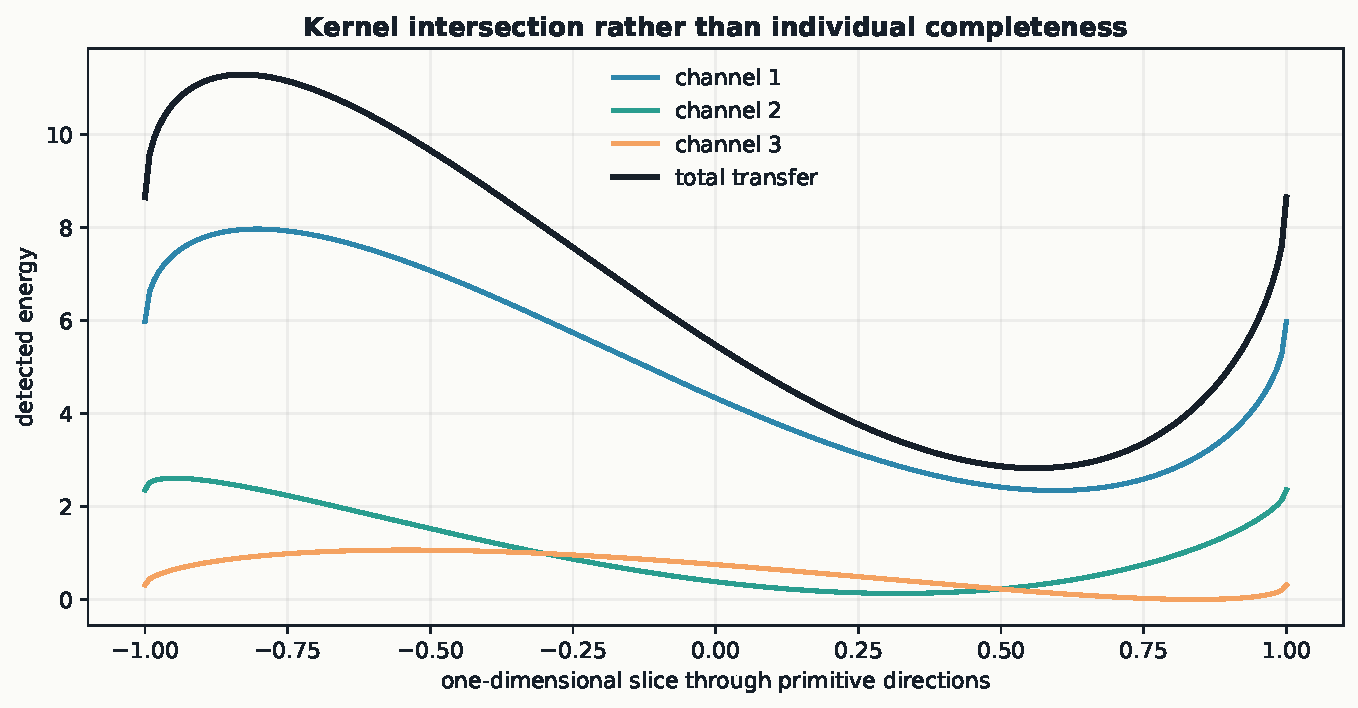
\includegraphics[width=0.82\textwidth]{17_multi_incidence_kernel_intersection.pdf}
\caption{The correct criterion is the vanishing of the joint kernel, not completeness of one channel.}
\end{figure}

\begin{corollary}[Finite Gram certificate]
Choose a rational basis $e_1,\ldots,e_d$ of $V$. If
\[
G_{ij}=\sum_r\langle A_re_i,A_re_j\rangle_{Y_r}
\]
has nonzero determinant, every rational Hodge class in $V$ is algebraic.
\end{corollary}

\chapter{Family propagation}
Let $\pi:\mathcal X\to S$ and $\rho_r:\mathcal Y_r\to S$ be smooth projective families over a connected base. Relative algebraic correspondences induce morphisms of Gauss-Manin local systems. In a flat rational trivialization, their transfer matrix is constant.

\begin{theorem}[Propagation of invertibility]
If a relative transfer $T_s$ is invertible on one fiber $s_0$, it is invertible on every fiber in the connected base on which the local systems and correspondences are defined.
\end{theorem}
\begin{proof}
The determinant of the constant rational matrix representing the local-system morphism is locally constant. It is nonzero at $s_0$, hence everywhere on the connected base.
\end{proof}

\begin{figure}[htbp]
\centering
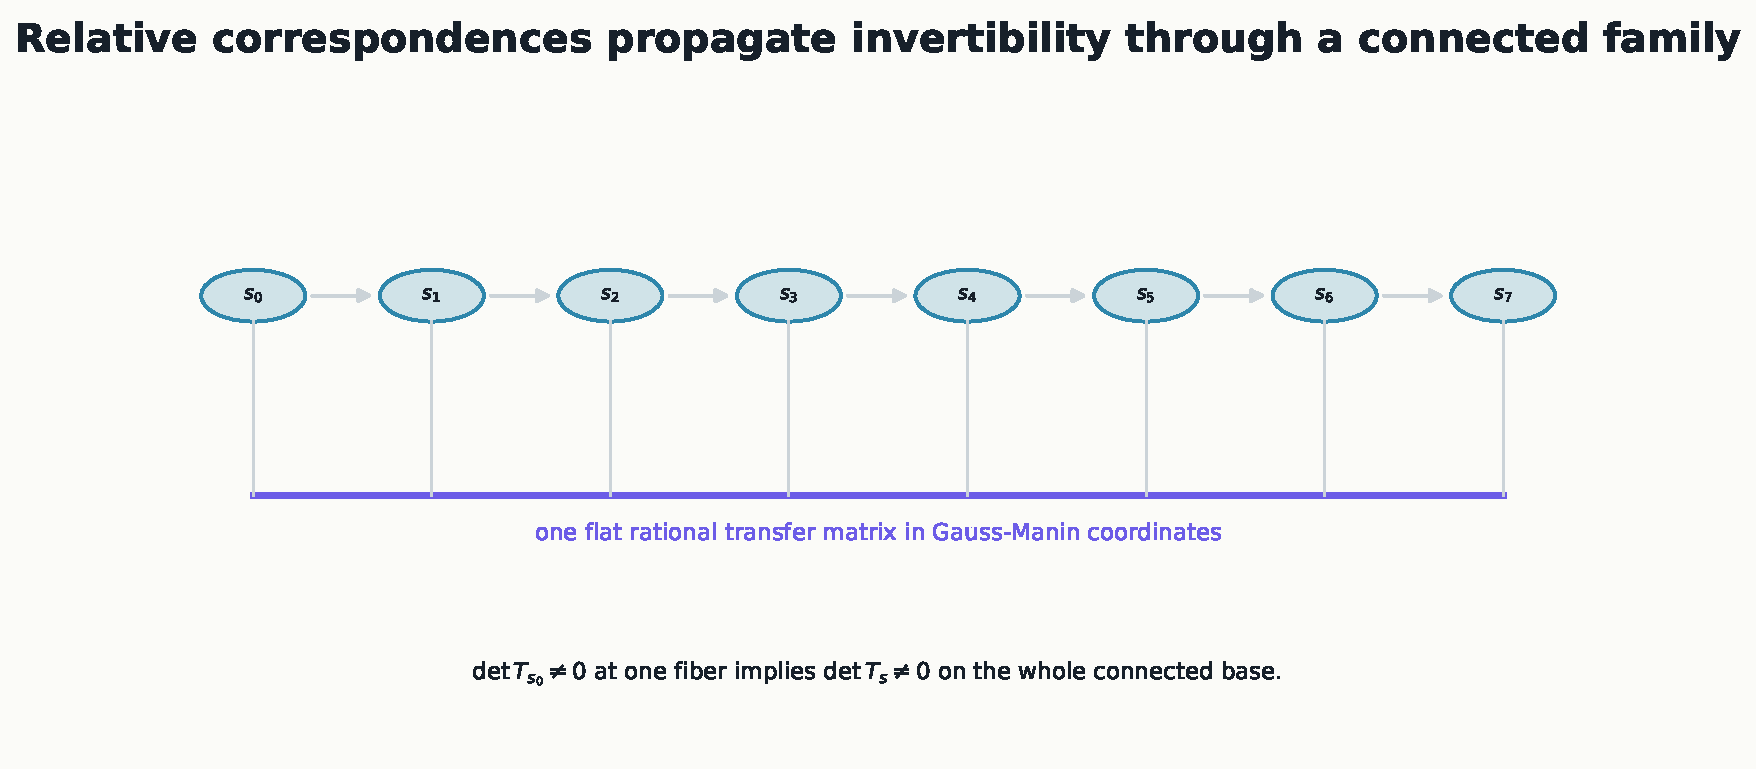
\includegraphics[width=0.83\textwidth]{19_family_propagation.pdf}
\caption{One verified fiber can control a connected smooth family when the correspondence is relative and flat.}
\end{figure}

\addcontentsline{toc}{part}{Part IV. Closed branches and classical validation cases}

\chapter{Geometric closure rules}
\section{Affine pavings}
\begin{theorem}[Affine-paving branch]
If $X$ admits a finite filtration whose successive differences are affine spaces, then the cycle class map
\[
\CH^p(X)_{\Q}\to H^{2p}(X,\Q)
\]
is surjective for every $p$.
\end{theorem}
\begin{proof}[Proof sketch]
Induct through the filtration using localization for Chow groups and cohomology. Each affine cell contributes one even-degree generator represented by the closure of that cell. No odd cohomology is introduced.
\end{proof}

\section{Projective bundles, blow-ups, and descent}
\begin{proposition}[Projective-bundle closure]
If the rational Hodge conjecture holds for $X$, it holds for $\mathbb P(E)\to X$.
\end{proposition}
\begin{proof}
The projective-bundle formula expresses cohomology as a direct sum of powers of the algebraic hyperplane class times pullbacks of cohomology from $X$.
\end{proof}

\begin{proposition}[Blow-up closure]
If it holds for $X$ and a smooth center $Z$, it holds for $\operatorname{Bl}_ZX$.
\end{proposition}
\begin{proof}
Use the standard blow-up cohomology decomposition. The new summands are Tate twists of cohomology from $Z$ multiplied by powers of the algebraic exceptional divisor.
\end{proof}

\begin{proposition}[Generically finite descent]
Let $f:Y\to X$ be proper and generically finite of degree $d$ between smooth projective varieties of equal dimension. If the conjecture holds for $Y$, it holds for $X$.
\end{proposition}
\begin{proof}
For a Hodge class $\alpha$ on $X$, the pullback $f^*\alpha$ is algebraic on $Y$. Push forward and use $f_*f^*\alpha=d\alpha$.
\end{proof}

\begin{figure}[htbp]
\centering
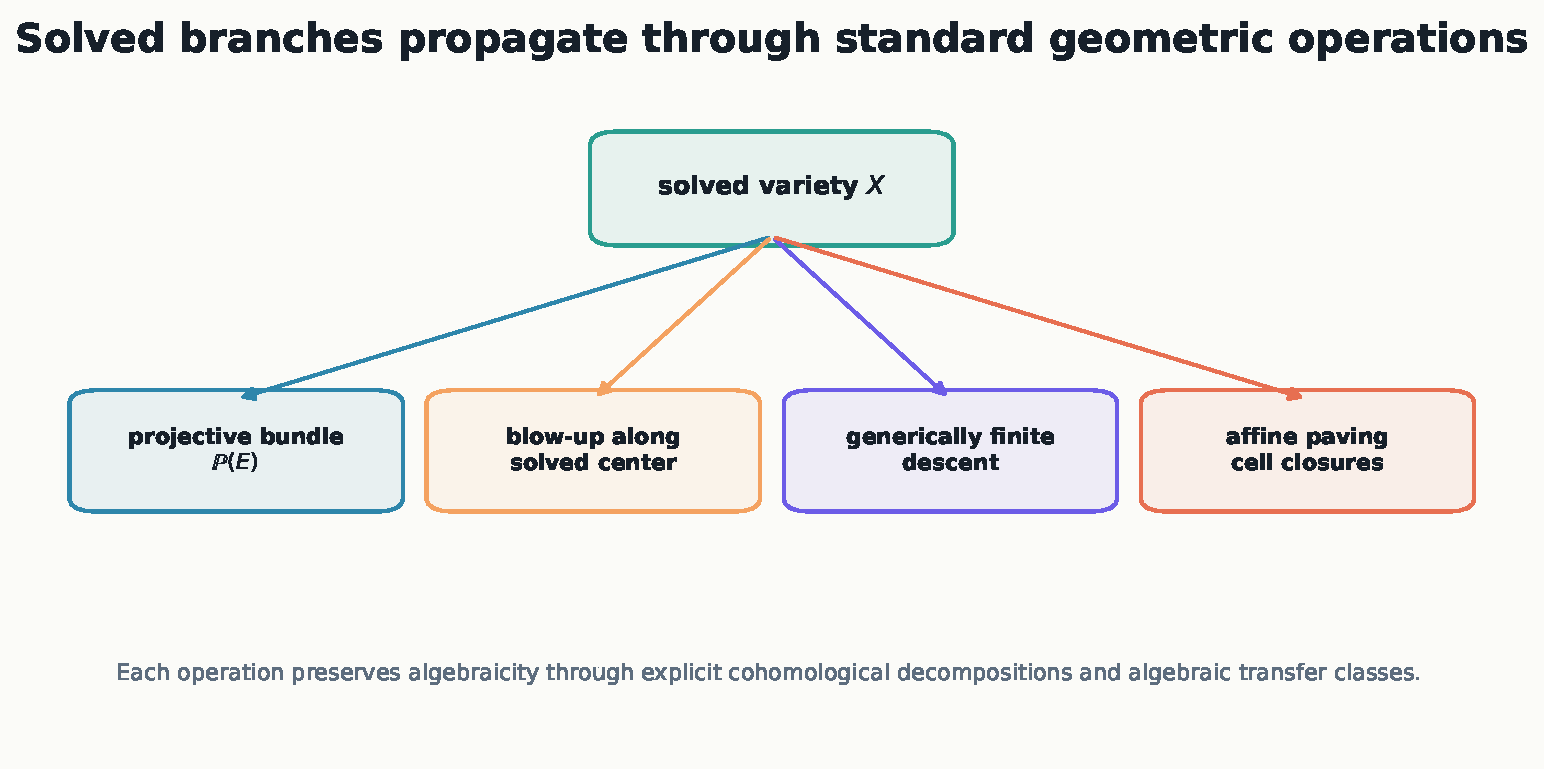
\includegraphics[width=0.84\textwidth]{20_geometric_closure_operations.pdf}
\caption{Solved branches propagate through several exact algebraic operations.}
\end{figure}

\chapter{Cubic fourfolds as a validation of the transfer theorem}
Let $X\subset\mathbb P^5$ be a smooth cubic fourfold and let $F(X)$ be its Fano variety of lines. The universal incidence variety
\[
P=\{(\ell,x):x\in\ell\}\subset F(X)\times X
\]
induces the Abel-Jacobi map
\[
A=p_*q^*:H^4_{\mathrm{prim}}(X,\Q)\to H^2_{\mathrm{prim}}(F(X),\Q).
\]
Beauville and Donagi proved that this is a polarized Hodge isomorphism up to the standard twist \cite{BeauvilleDonagi}. The polarized adjoint is represented by an algebraic incidence return after inserting the appropriate power of the Pluecker class. Therefore the divisor-lowering transfer is invertible.

\begin{resultbox}[Classical validation]
A primitive rational $(2,2)$ class on a cubic fourfold is sent to a rational $(1,1)$ class on $F(X)$, represented by a divisor. The algebraic return correspondence and its polynomial inverse reconstruct an algebraic codimension-two class on $X$. This is a validation of the packet criterion, not a claim of a new proof of the classical cubic-fourfold result.
\end{resultbox}

\begin{figure}[htbp]
\centering
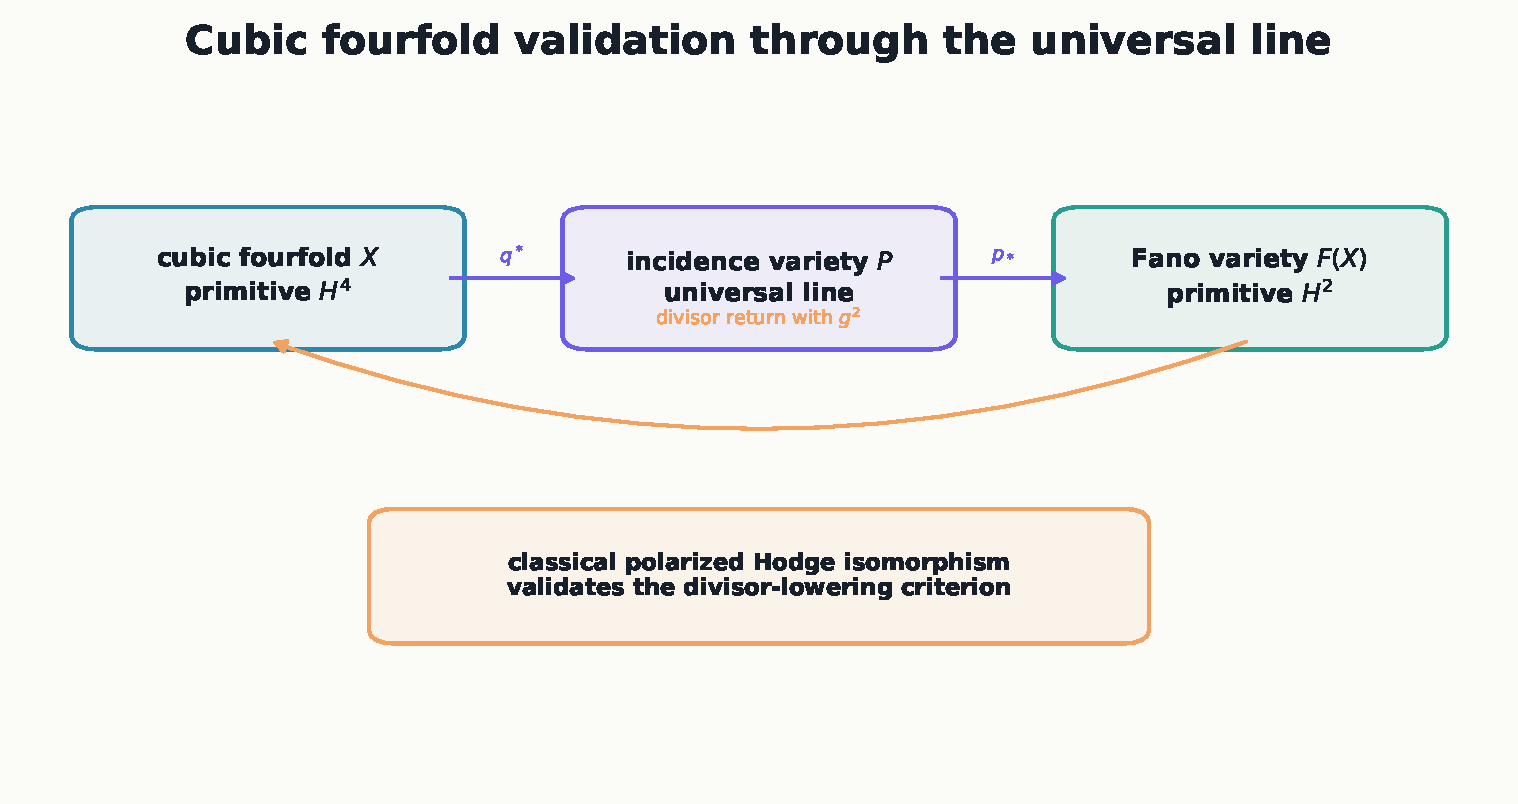
\includegraphics[width=0.86\textwidth]{21_cubic_fourfold_incidence.pdf}
\caption{The universal line lowers primitive degree-four cohomology to divisor degree on the Fano variety.}
\end{figure}

\begin{figure}[htbp]
\centering
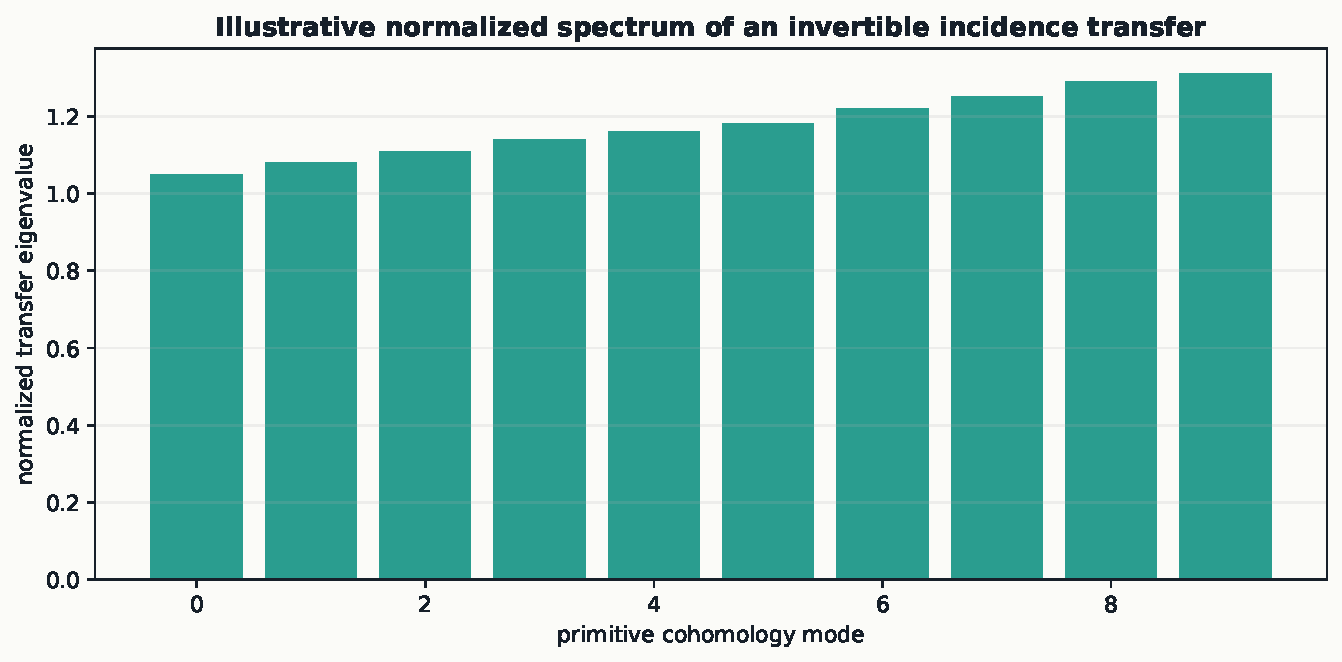
\includegraphics[width=0.72\textwidth]{22_cubic_transfer_spectrum.pdf}
\caption{Illustrative normalized transfer spectrum. The mathematical criterion is nonvanishing, not the displayed toy values.}
\end{figure}

\chapter{Gushel-Mukai validation channels}
Debarre and Kuznetsov construct line and plane incidence correspondences relating vanishing middle cohomology of suitable Gushel-Mukai varieties to primitive degree-two cohomology of associated double EPW sextics \cite{DebarreKuznetsov}. In the ranges where the polarized Hodge isomorphisms are established, the same divisor-lowering theorem applies.

\begin{itemize}
\item For suitable GM fourfolds, the vanishing $H^4$ packet is lowered by universal lines to divisor degree.
\item For suitable GM sixfolds, the vanishing $H^6$ packet is lowered by universal planes to divisor degree.
\item Ambient and tautological classes are treated separately and are algebraic.
\end{itemize}

\begin{figure}[htbp]
\centering
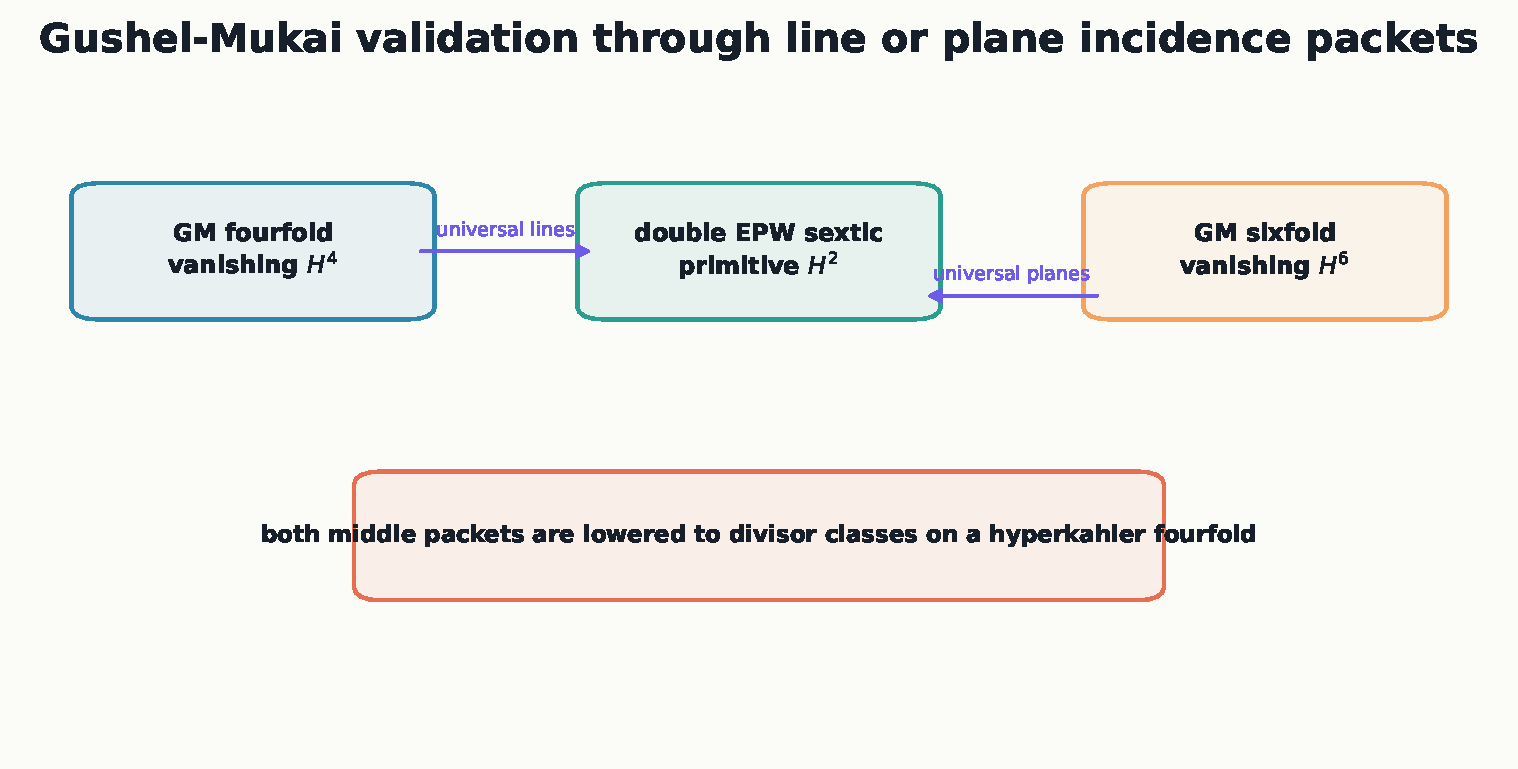
\includegraphics[width=0.84\textwidth]{23_gushel_mukai_correspondences.pdf}
\caption{Line and plane incidence packets lower middle cohomology to degree two on an associated hyperkaehler fourfold.}
\end{figure}

\addcontentsline{toc}{part}{Part V. The analytic and K-theoretic branch}

\chapter{Hodge packets in topological K-theory}
For finite CW complexes, the rational topological Chern character gives
\[
\operatorname{ch}_{\mathrm{top}}:K^0_{\mathrm{top}}(X)\otimes\Q\xrightarrow{\sim}H^{\mathrm{even}}(X,\Q).
\]
For smooth projective $X$, the algebraic Chern character identifies algebraic $K$-theory rationally with the Chow ring after the usual filtration. Thus the rational Hodge conjecture for all degrees is equivalent to algebraization of topological $K$-classes whose Chern-character components are rational Hodge classes \cite{AtiyahHirzebruch}.

\section{Adams degree projectors}
For integer $m\ge2$, Adams operations satisfy
\[
\operatorname{ch}_q(\psi^m\xi)=m^q\operatorname{ch}_q(\xi).
\]
Define
\[
e_p^{(m)}=\prod_{\substack{0\le q\le\dim X\\q\ne p}}
\frac{\psi^m-m^qI}{m^p-m^q}.
\]
Then
\[
\operatorname{ch}_q(e_p^{(m)}\xi)=\delta_{pq}\operatorname{ch}_p(\xi).
\]
This exactly isolates codimension $p$ inside a topological $K$-packet.

\begin{figure}[htbp]
\centering
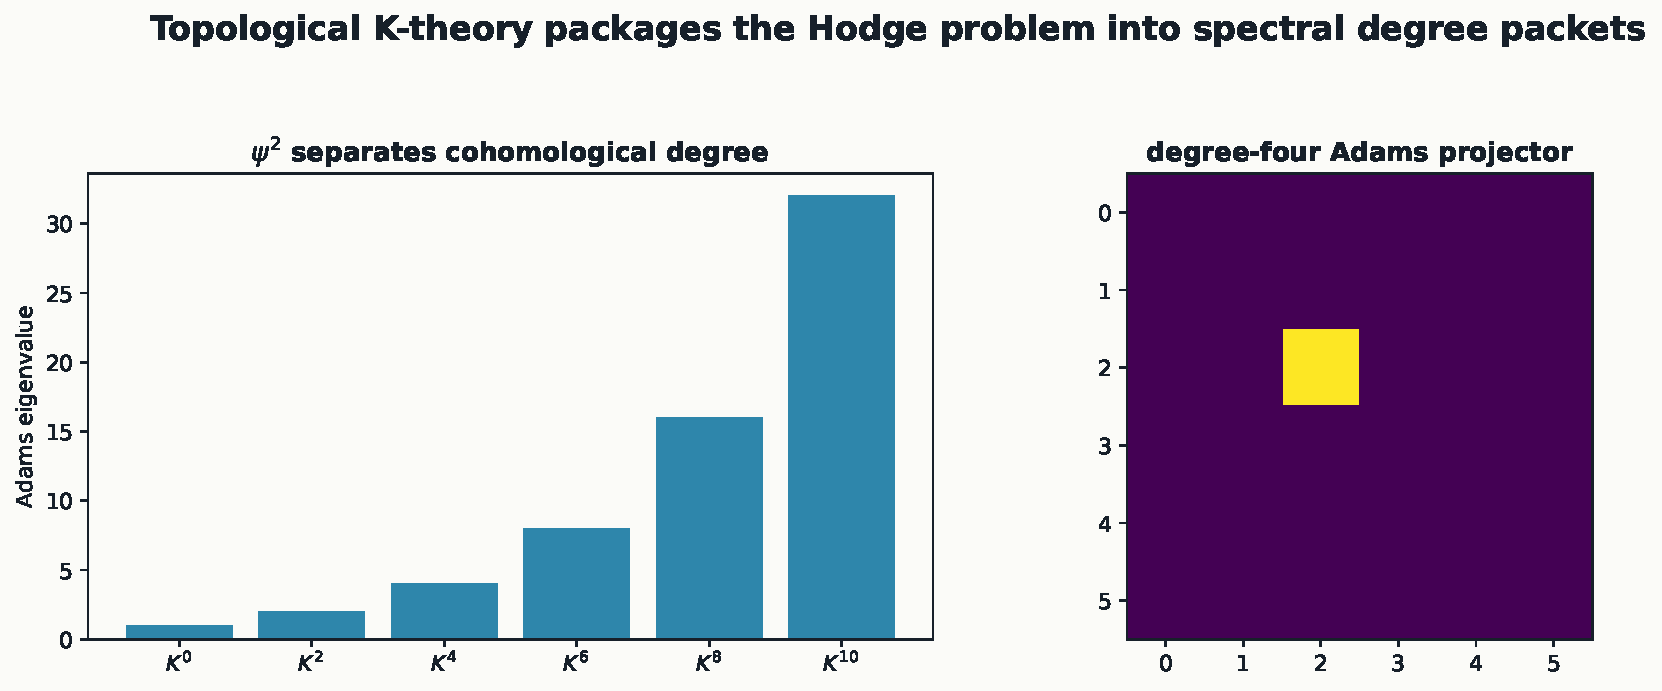
\includegraphics[width=0.86\textwidth]{24_adams_degree_projector.pdf}
\caption{Adams eigenvalues separate cohomological degrees and yield an exact spectral projector onto degree four in the toy model.}
\end{figure}

\chapter{Nonlinear Dolbeault obstruction packets}
Let $E$ be a smooth complex bundle and consider a candidate $(0,1)$-connection. After gauge fixing, write the integrability equation abstractly as
\[
F(a)=f+La+B(a,a)=0,
\]
where $L$ is the linearized operator and $B$ is a bounded bilinear term. Assume a Fredholm splitting of the target
\[
I=Q+\Pi,
\]
where $Q$ projects onto the range of $L$ and $\Pi$ onto a finite-dimensional obstruction space. Let $R$ be a right inverse of $L$ on the range.

\begin{theorem}[Range-packet contraction]
Assume
\[
\|R\|\le M,
\qquad
\|B(a,b)\|\le C\|a\|\|b\|,
\qquad
4CM^2\|Qf\|<1.
\]
Then the map
\[
\mathcal T(a)=-RQ(f+B(a,a))
\]
has a unique fixed point in the ball $\|a\|\le2M\|Qf\|$. At the fixed point, the range component of $F(a)$ vanishes. The remaining obstruction is
\[
\Phi=\Pi(f+B(a,a)).
\]
The full integrability equation holds if and only if $\Phi=0$.
\end{theorem}
\begin{proof}
For $\|a\|\le r=2M\|Qf\|$,
\[
\|\mathcal T(a)\|\le M\|Qf\|+MC r^2\le r
\]
under the stated bound. Moreover
\[
\|\mathcal T(a)-\mathcal T(b)\|
\le MC(\|a\|+\|b\|)\|a-b\|<\|a-b\|.
\]
Banach's fixed-point theorem gives the solution. Applying $Q$ to the equation proves range cancellation. The remaining component is precisely $\Phi$.
\end{proof}

\begin{figure}[htbp]
\centering
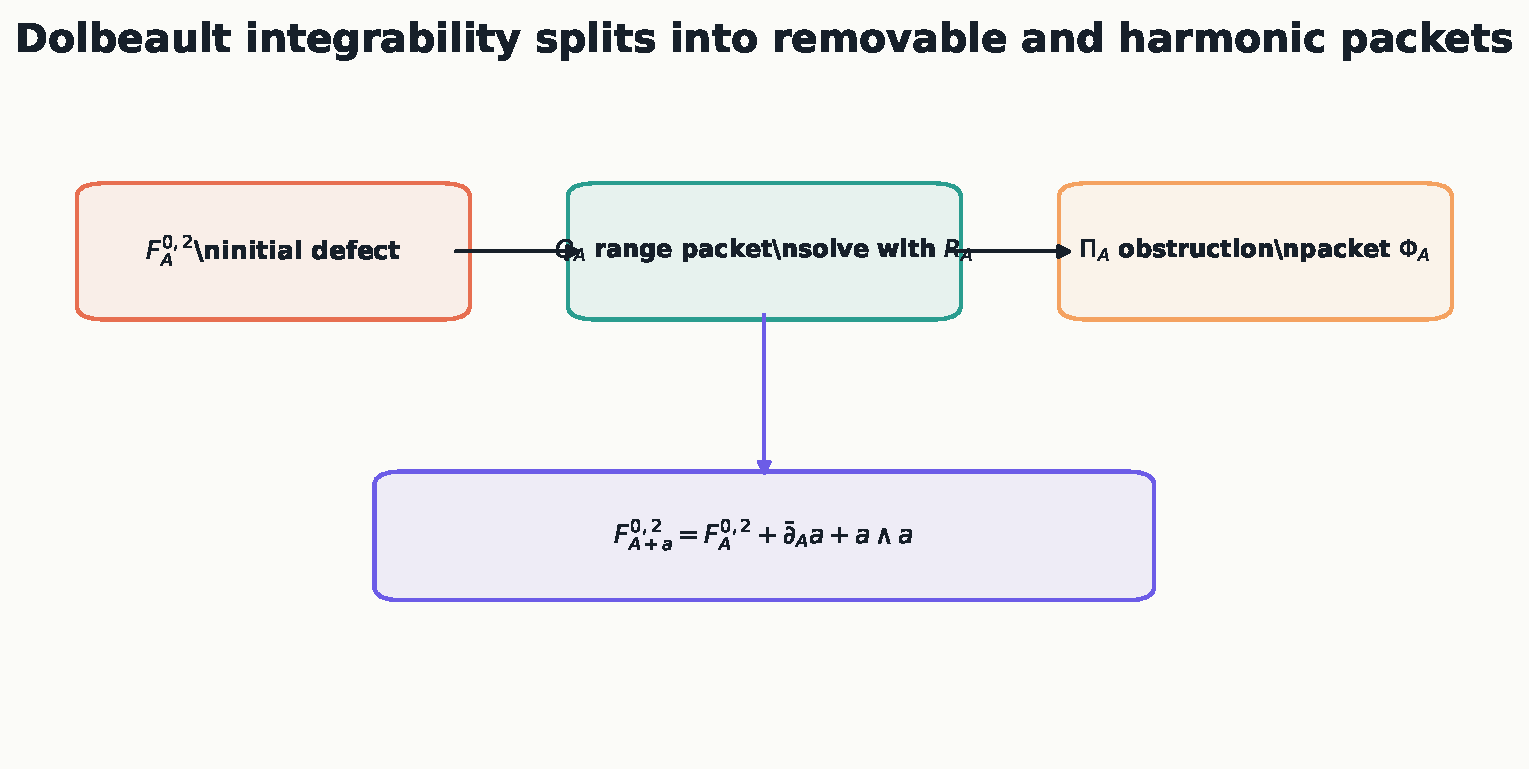
\includegraphics[width=0.84\textwidth]{25_dolbeault_obstruction_split.pdf}
\caption{The nonlinear equation splits into a removable range packet and a finite effective obstruction packet.}
\end{figure}

\begin{figure}[htbp]
\centering
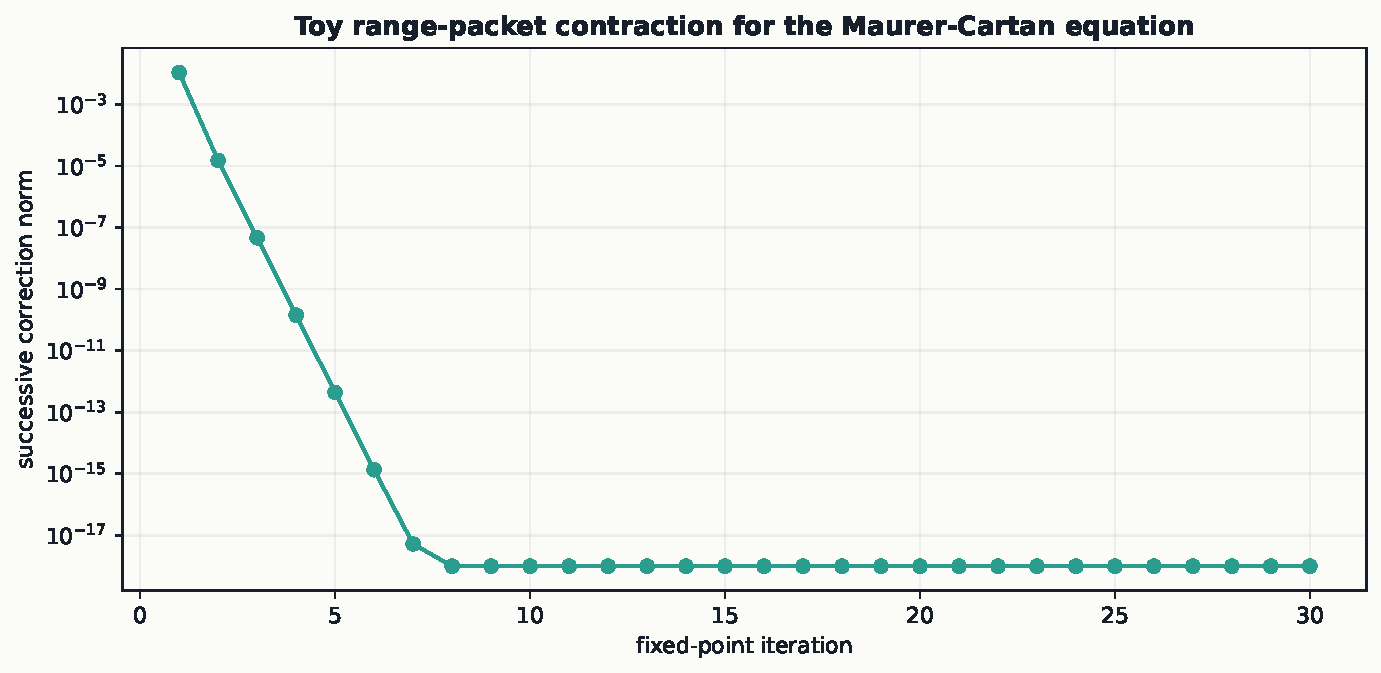
\includegraphics[width=0.72\textwidth]{26_dolbeault_contraction.pdf}
\caption{Reproducible finite model of geometric contraction in the removable packet.}
\end{figure}

\section{A positive spectral microscope}
Large ample twists can make integrability defects visible in the asymptotic degree distribution of Dolbeault-Dirac kernels. Charbonneau and Stern obtain asymptotic Hodge filtrations in which positive coefficients depend on powers of $F_A^{0,2}$ \cite{CharbonneauStern}. Schematically,
\[
\Tr(P_{2j}\Pi_{A,k})
=c_{n,j}k^{n-2j}\|(F_A^{0,2})^{\wedge j}\|_{L^2}^2+O(k^{n-2j-1}),
\qquad c_{n,j}>0.
\]
This detects nonintegrability. It does not by itself remove the defect.

\begin{figure}[htbp]
\centering
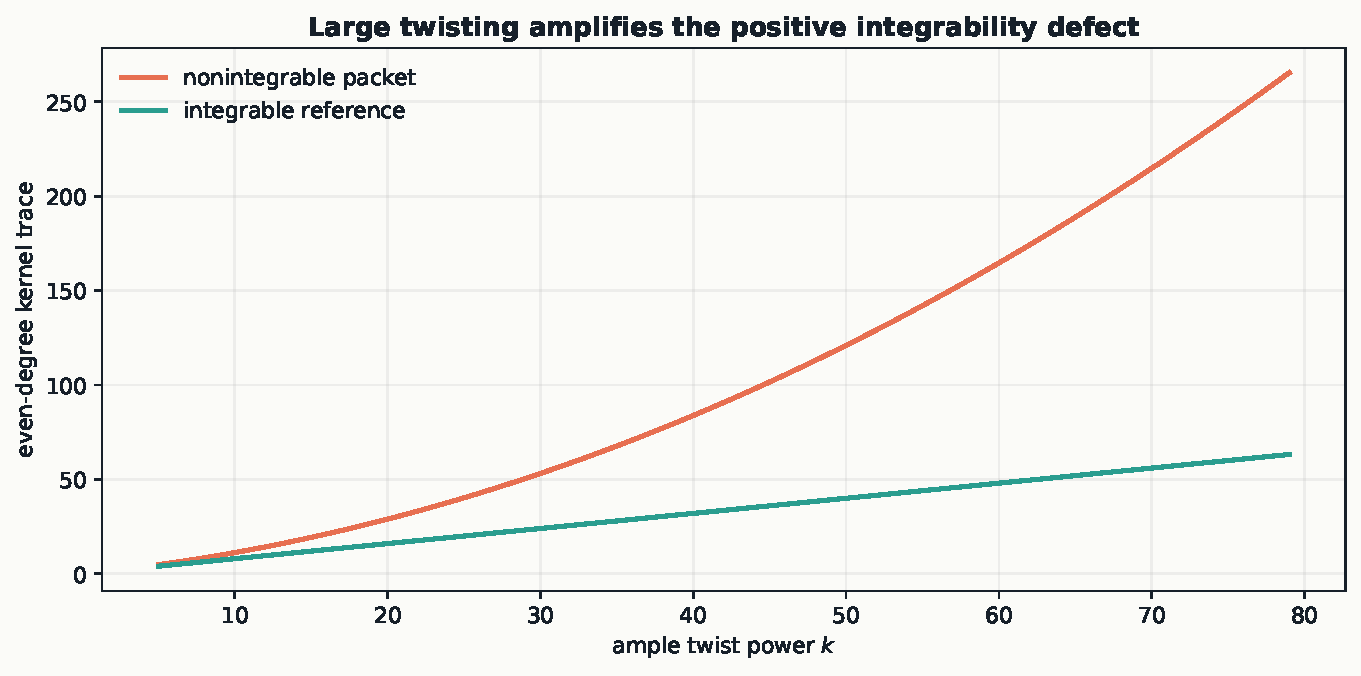
\includegraphics[width=0.74\textwidth]{27_asymptotic_integrability_packet.pdf}
\caption{Ample twisting acts as a spectral microscope for a positive integrability defect.}
\end{figure}

\section{Trace blindness and the true missing bridge}
Chern characters control traces of powers of curvature. An endomorphism-valued obstruction can be nonzero while all such trace moments vanish. A nilpotent block gives the elementary counterexample.

\begin{figure}[htbp]
\centering
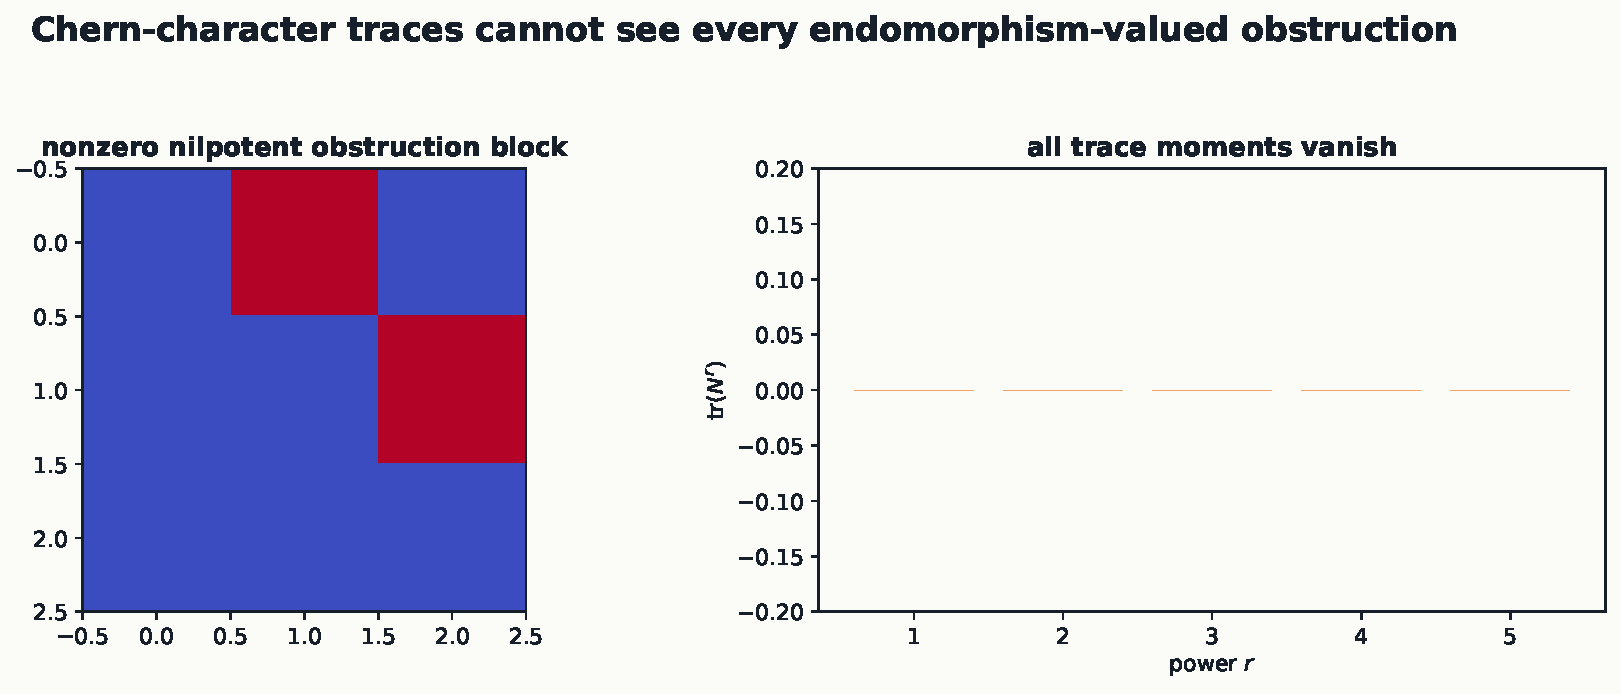
\includegraphics[width=0.8\textwidth]{28_trace_blindness.pdf}
\caption{A nonzero nilpotent obstruction can be invisible to every trace power. Hodge-type Chern data do not automatically kill the full matrix obstruction.}
\end{figure}

\begin{openproblem}[Analytic bridge]
The unresolved analytic theorem is not the range equation. It is a positive saturation statement forcing the finite obstruction packet $\Phi$ to vanish for every rational Hodge $K$-packet after allowable stabilization. Proving that statement in general would be essentially a K-theoretic form of the Hodge conjecture.
\end{openproblem}

\section{Consequences of the obstruction split}
The obstruction split prevents a common logical error. Solving the projected range equation does not solve the original integrability problem unless the complementary packet also vanishes. The calculus therefore records three distinct outcomes. First, if $\Pi=0$, the problem is unobstructed and the contraction theorem gives an actual integrable structure. Second, if $\Pi\ne0$ but $\Phi=0$ for geometric reasons, the correction again closes. Third, if $\Phi\ne0$, the method has produced a finite certificate explaining exactly why that representative cannot be algebraized by the chosen deformation.

This creates a practical research program. One can refine the finite obstruction space by symmetry, monodromy, support, or arithmetic phase, obtaining
\[
\Phi=\sum_{\lambda}\Phi_{\lambda}.
\]
Since the decomposition is complete, integrability is equivalent to the simultaneous vanishing of all children. Different geometric arguments may eliminate different children. A symmetry packet may vanish by representation theory, a support packet by localization, and an arithmetic packet by compatibility across reductions. The analytic branch therefore remains useful even before the general bridge is proved: it supplies exact special-case theorems whenever all obstruction children can be eliminated.

The negative controls are equally important. Ample twisting can amplify $F_A^{0,2}$ in a spectral observable without reducing it. Direct-sum stabilization adds positive defect energies for block-diagonal connections. Trace identities may miss nilpotent components. These facts rule out several tempting but invalid shortcuts and keep the remaining theorem sharply stated.


\addcontentsline{toc}{part}{Part VI. Atomic status ledger and focused next theorem}

\chapter{Dependency graph and proof status}
The project separates proved statements, classical inputs, conditional mechanisms, and open bridges.

\begin{figure}[htbp]
\centering
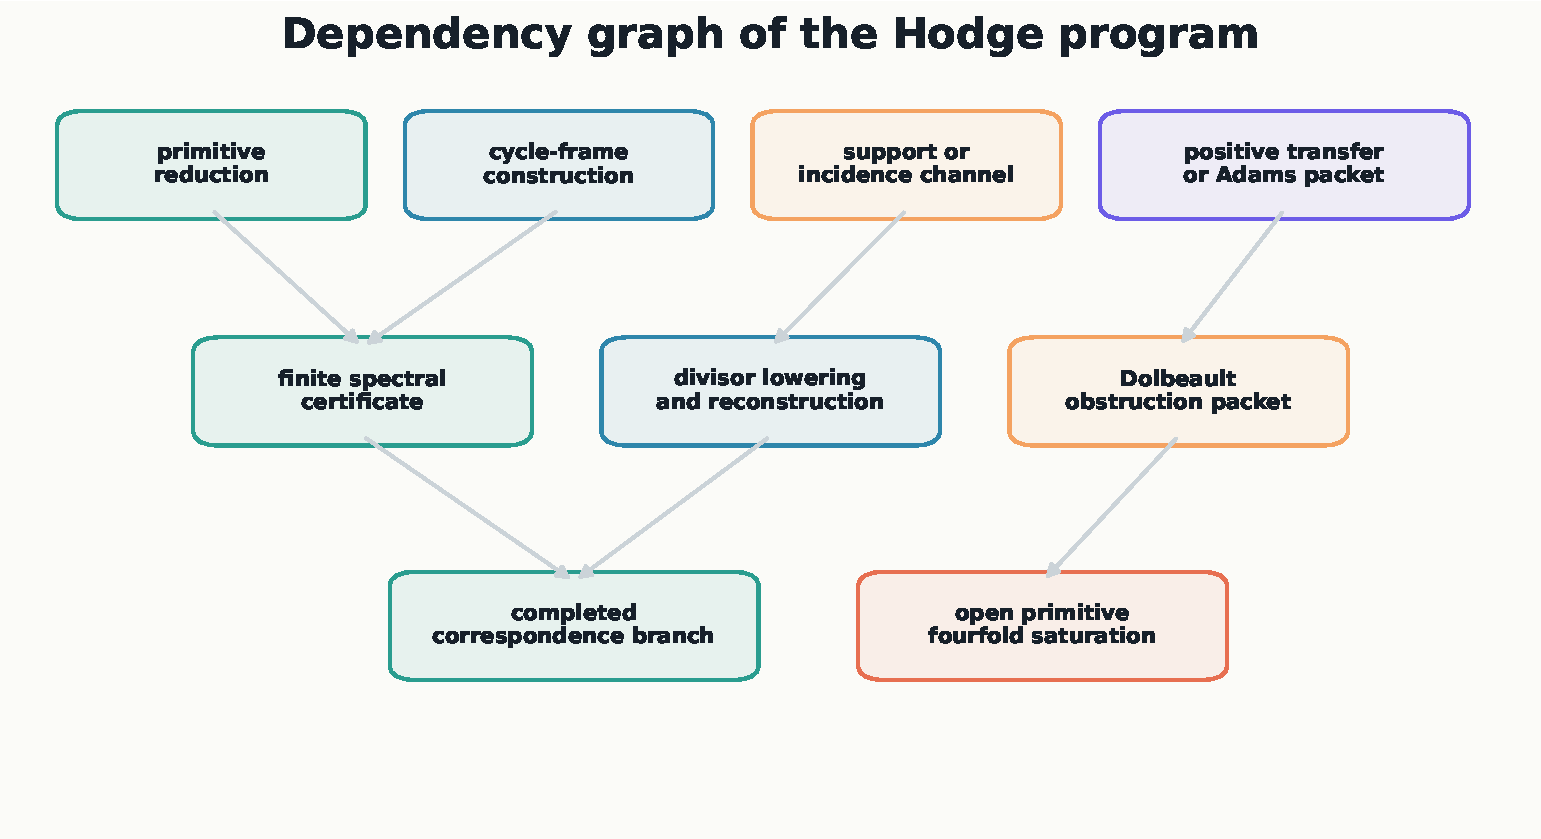
\includegraphics[width=0.92\textwidth]{29_hodge_dependency_graph.pdf}
\caption{Dependency graph. The correspondence branch is complete under an explicit invertible transfer, while primitive fourfold saturation remains open.}
\end{figure}

\begin{longtable}{p{0.40\textwidth}p{0.16\textwidth}p{0.34\textwidth}}
\caption{Atomic status ledger.}\label{tab:status}\\
\toprule
Statement & Status & Boundary \\
\midrule
\endfirsthead
\toprule
Statement & Status & Boundary \\
\midrule
\endhead
Master obstruction projector & Proved & Finite-dimensional linear algebra \\
Primitive Lefschetz reduction & Proved & Uses hard Lefschetz and algebraicity of the polarization \\
Degree-$2p$ coniveau identification & Proved & Rational coefficients and purity \\
Positive cycle-frame certificate & Proved & Requires an explicit finite cycle family \\
Exact degree polyphase assembly & Proved & Frame operators, not sums of span projectors \\
Finite saturation of bounded-degree spans & Proved & Non-effective degree bound \\
Support verification & Proved & Candidate support must already be supplied \\
Multiplicity reconstruction & Proved & Finite rational linear algebra \\
Divisor-lowering transfer theorem & Proved & Requires explicit algebraic correspondences and invertibility \\
Positive multi-channel criterion & Conditional & Algebraic realization of polarized adjoints is an extra hypothesis \\
Family propagation & Proved & Relative correspondences over a connected smooth base \\
Affine-paving branch & Proved & Classical localization argument \\
Projective bundle, blow-up, descent rules & Proved & Standard cohomological decompositions \\
Cubic and GM channels & Classical validation & Depend on established incidence Hodge isomorphisms \\
Adams degree projector & Proved & Rational topological K-theory \\
Range-packet nonlinear correction & Proved under hypotheses & Closed range, right inverse, and contraction bound \\
Vanishing of every harmonic obstruction packet & Open & Main analytic bridge \\
Primitive fourfold multi-incidence saturation & Open & Main geometric target \\
General rational Hodge conjecture & Open & No general cycle-generation theorem is claimed \\
\bottomrule
\end{longtable}

\begin{figure}[htbp]
\centering
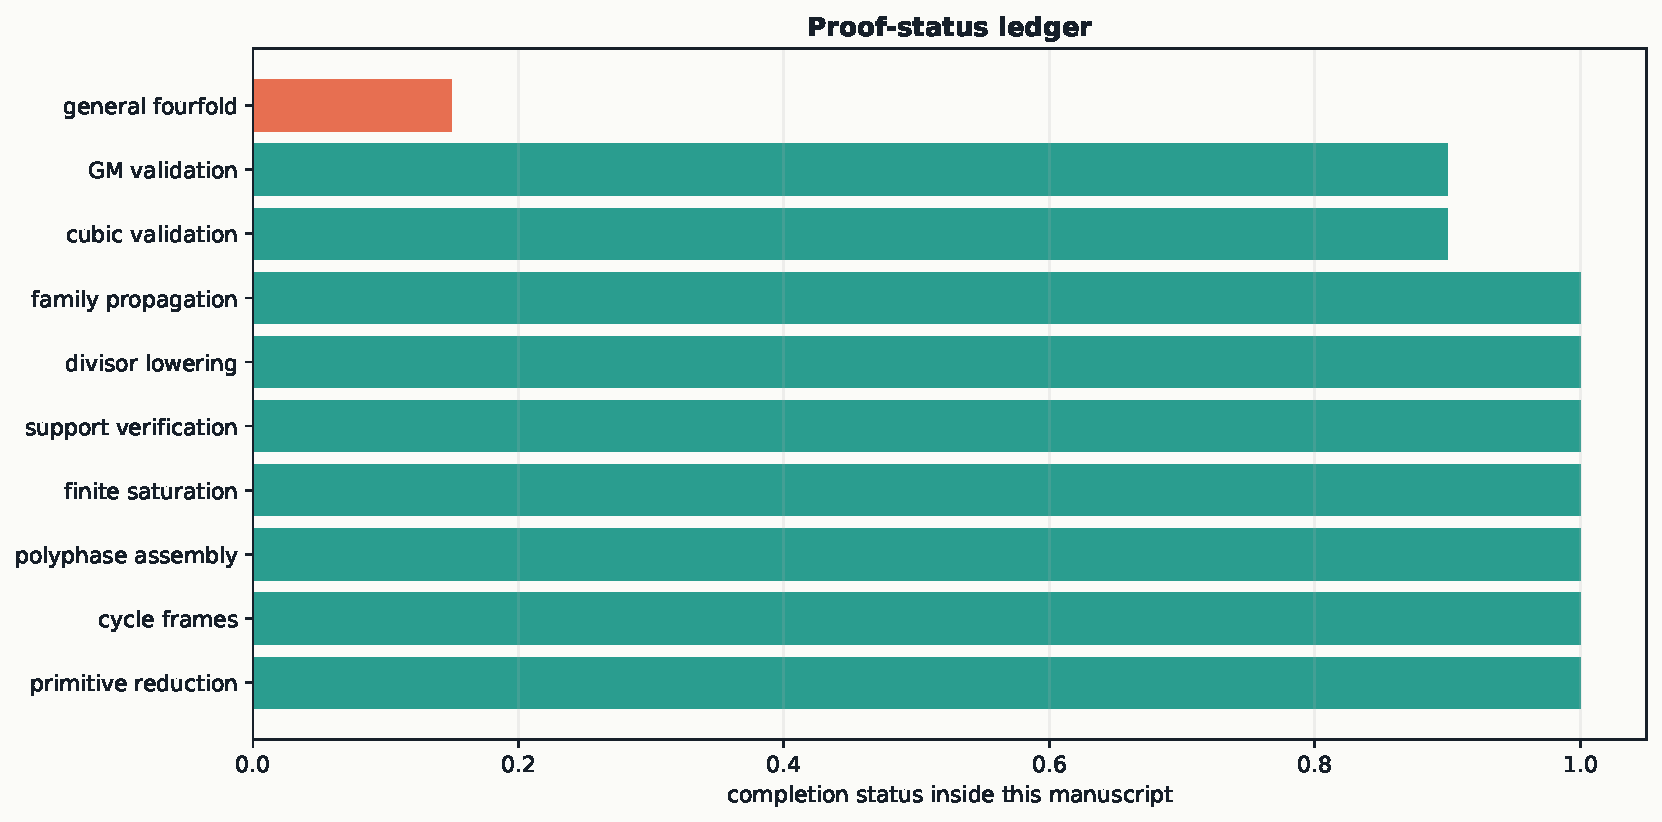
\includegraphics[width=0.78\textwidth]{32_status_ledger.pdf}
\caption{Visual status ledger for the finite core, validation cases, and open general target.}
\end{figure}

\chapter{The next realistic theorem: multi-incidence saturation}
Let $X$ be a special smooth projective fourfold. Construct algebraic lowering channels from families of subvarieties:
\[
A_{\mathrm{line}},
A_{\mathrm{conic}},
A_{\mathrm{plane}},
A_{\mathrm{exceptional}}.
\]
The exact target is
\[
\ker A_{\mathrm{line}}
\cap\ker A_{\mathrm{conic}}
\cap\ker A_{\mathrm{plane}}
\cap\ker A_{\mathrm{exceptional}}=\{0\}
\]
on primitive degree-four cohomology. Under algebraic adjoint hypotheses, equivalently prove
\[
T_{\mathrm{tot}}
=\sum_rA_r^\dagger A_r
\quad\text{satisfies}\quad
\lambda_{\min}(T_{\mathrm{tot}})>0.
\]

\begin{figure}[htbp]
\centering
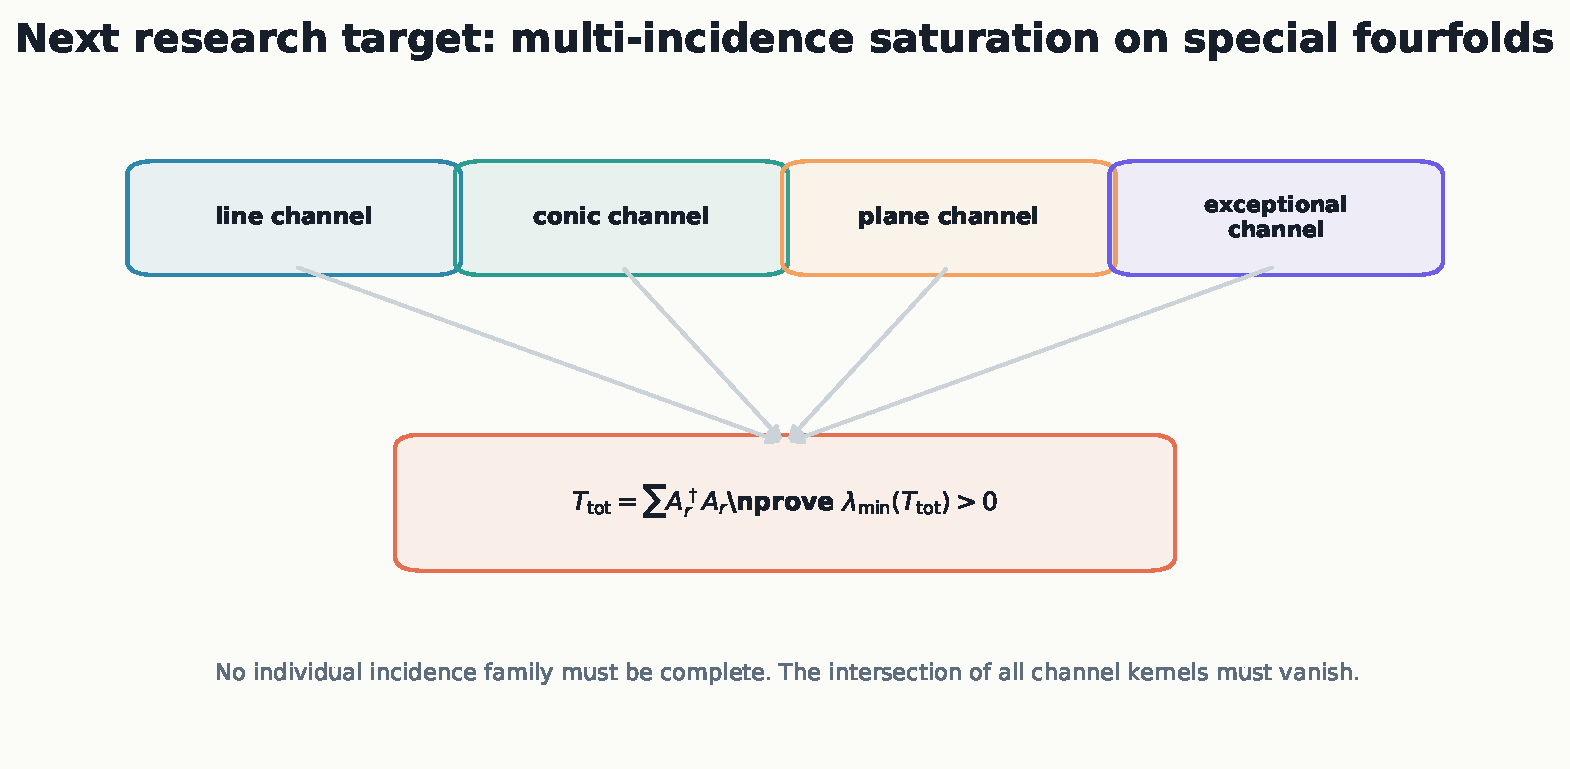
\includegraphics[width=0.86\textwidth]{30_multi_incidence_target.pdf}
\caption{The focused next theorem combines multiple incomplete incidence spaces into one positive saturating transfer.}
\end{figure}

\section{Why this target is realistic}
The problem is finite after the geometry is chosen:
\begin{enumerate}
\item compute the primitive cohomology representation and its symmetry decomposition
\item construct the incidence correspondences and their action
\item split the action into monodromy or symmetry packets
\item compute the joint kernel or positive Gram matrix over $\Q$
\item prove exact nonvanishing through rational rank, representation theory, or a dual certificate
\item invoke the divisor-lowering theorem to reconstruct cycles
\end{enumerate}
No single incidence family must be complete. Polyphase analysis permits separate geometric mechanisms to occupy separate primitive sectors.


\section{Three exact certificate forms}
Once the incidence channels have been constructed, the saturation statement admits three finite certificates. The geometric form is the kernel identity
\[
\bigcap_r\ker A_r=\{0\}.
\]
When algebraic correspondences realize the polarized adjoints, the equivalent positive form is
\[
\lambda_{\min}\left(\sum_rA_r^\dagger A_r\right)>0.
\]
In a rational basis, the final exact proof object is full column rank of the vertically stacked channel matrix. The kernel form explains the geometry, the positive form is stable for numerical scouting, and the rational rank form is appropriate for symbolic certification.

Two negative controls should accompany the proof. First, remove one channel at a time and recompute the joint kernel. If the kernel grows, the omitted incidence family is genuinely necessary. Second, refine a parent channel into geometric children and verify that their positive transfers sum exactly to the parent. This separates true packet coverage from accidental numerical invertibility.

A complete result should identify which primitive symmetry packets are detected by lines, conics, planes, or exceptional strata. The proof then becomes a finite occupancy statement: every primitive packet must be detected at least once. That structural description is more informative than a determinant alone and is the form most likely to propagate through families and degenerations.

\chapter{Computational and formal proof workflow}
Numerical experiments can scout candidate families but cannot replace an exact rank certificate. The intended pipeline is:
\[
\begin{aligned}
\text{exact incidence data}
&\longrightarrow \text{rational cohomology basis}
\longrightarrow \text{packet transfer matrices}\\
&\longrightarrow \text{rank or positivity certificate}
\longrightarrow \text{symbolic theorem proof}.
\end{aligned}
\]

\begin{figure}[htbp]
\centering
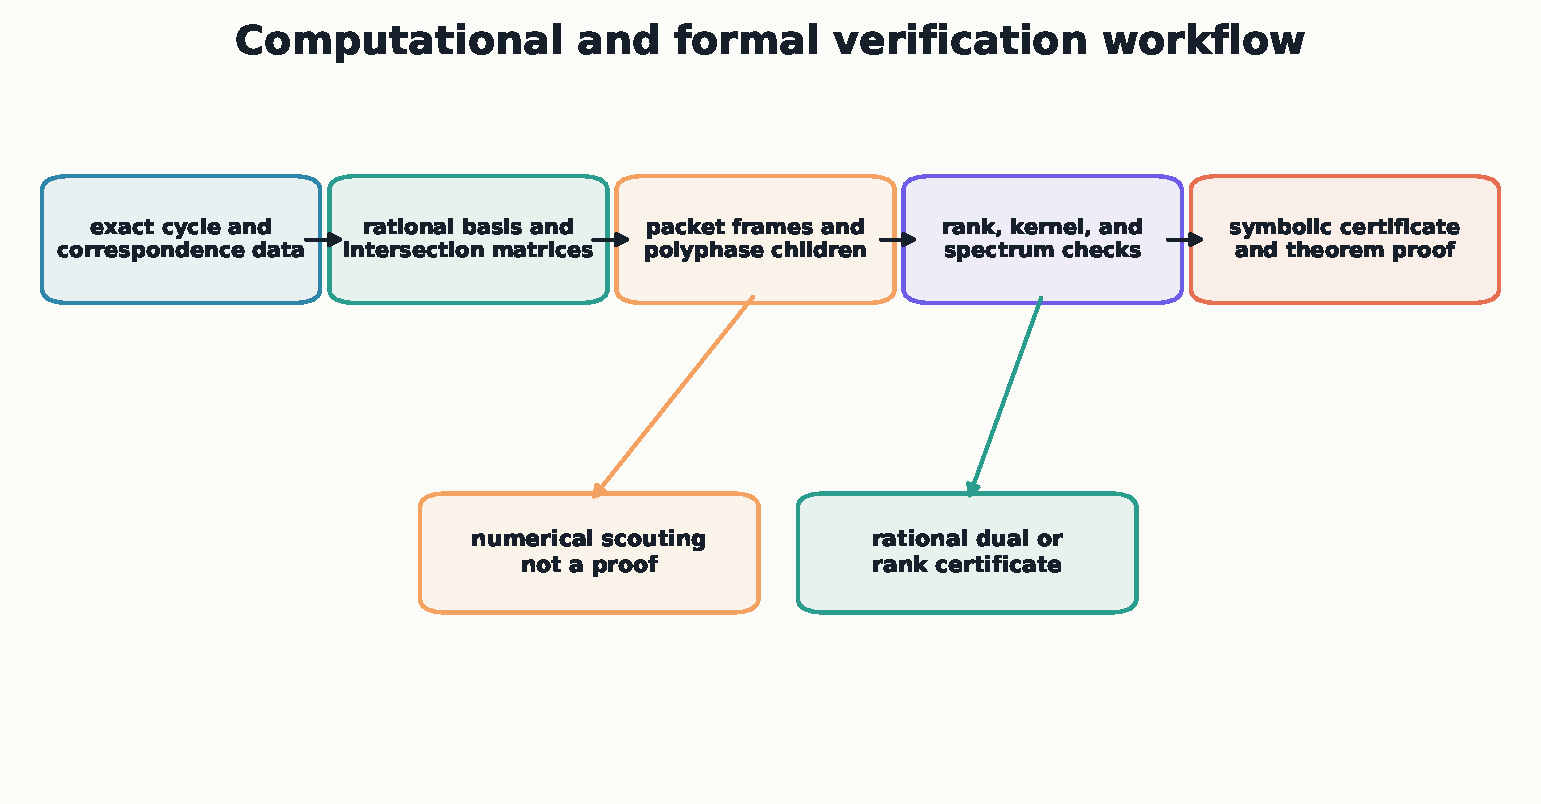
\includegraphics[width=0.9\textwidth]{31_verification_workflow.pdf}
\caption{Numerical scouting is separated from rational certification and formal theorem verification.}
\end{figure}

\section{Reproducible finite checks}
The accompanying Python generator produces all figures and runs eighteen independent finite checks covering:
\begin{itemize}
\item frame idempotency and range rank
\item positive Hodge Gram spectrum
\item exact modulo-$2$ and modulo-$4$ polyphase assembly
\item positive transfer rank and energy identities
\item Cayley-Hamilton inversion
\item contraction of the removable nonlinear packet
\item Adams projector idempotency and degree isolation
\item nilpotent trace blindness
\item support multiplicity recovery
\item finite rank stabilization
\end{itemize}
These tests verify the finite examples and implementation. They do not establish the open geometric saturation theorem.

\compactpart{Part VII. Fermat Fourfold Character Packets and the Constructive Program}

\chapter{Correct scope and claim boundary}
The projector-resolved Hodge calculus naturally specializes to Fermat fourfolds
\[
X_m^4=\{x_0^m+x_1^m+x_2^m+x_3^m+x_4^m+x_5^m=0\}\subset\mathbf P^5,
\qquad m\ge 3.
\]
The diagonal symmetry group makes the primitive middle cohomology unusually explicit: it splits into one-dimensional complex character lines, and rational Hodge packets are finite Galois orbits of those lines. This permits a complete symbolic analysis of addresses, conductors, local prime phases, and candidate algebraic correspondences.

\begin{claimboundary}
The general rational Hodge conjecture remains open. For Fermat fourfolds, however, Kang states a published generalized-Hodge theorem covering every degree \cite{KangFermat}. This complete edition therefore distinguishes two questions:
\begin{enumerate}
\item \emph{Existence}: does every rational Fermat $(2,2)$ class have an algebraic representative?
\item \emph{Construction}: can one write an explicit packet-resolved algebraic cycle or correspondence for every character orbit?
\end{enumerate}
The present Fermat program is primarily constructive. Its new proof objects are conductor projectors, exact packet identities, explicit Delsarte maps, weighted dyadic refinements, the all-degree trivalent-tree uniqueness theorem, CRT--Kummer phase factorizations, and explicit CM carrier data. The relation between that existence theorem and later packet-specific combinatorial work should be stated explicitly in any publication.
\end{claimboundary}

\begin{figure}[htbp]
\centering
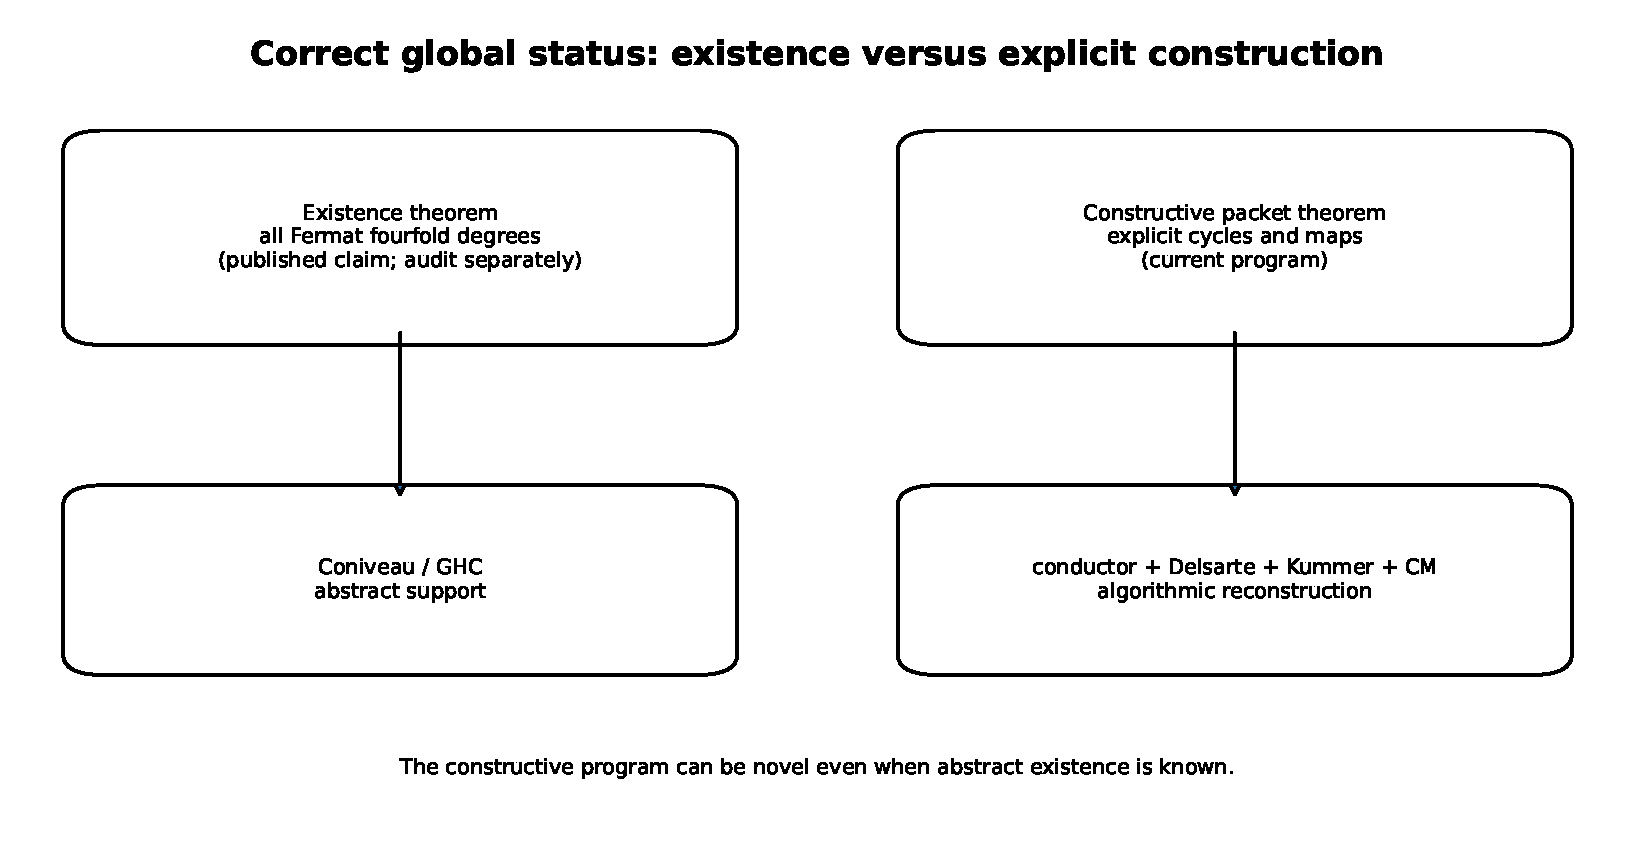
\includegraphics[width=0.90\textwidth]{41_status_correction.pdf}
\caption{The all-degree existence question and the packet-by-packet constructive question are logically distinct.}
\end{figure}

The constructive objective is
\begin{resultbox}[Packet-resolved construction target]
For every rational packet
\[
W\subset H^4_{\mathrm{prim}}(X_m^4,\Q)\cap H^{2,2},
\]
construct
\[
Z_W\in\CH^2(X_m^4)_\Q
\qquad\text{with}\qquad
[Z_W]\ne0\text{ in }W.
\]
\end{resultbox}
Once one nonzero algebraic vector is produced in a rational irreducible diagonal-symmetry packet, the entire rational orbit is algebraic.

\chapter{Universal balanced-packet equations}
Let
\[
U_m=(\mathbf Z/m\mathbf Z)^\times
\]
and let \(\langle r\rangle_m\in\{1,\ldots,m\}\) denote the least positive residue, with \(\langle r\rangle_m=m\) when \(m\mid r\). A primitive character address is a six-tuple
\[
a=(a_0,\ldots,a_5),\qquad 1\le a_i<m,
\qquad \sum_i a_i\equiv0\pmod m.
\]
The Hodge level of the conjugate indexed by \(u\in U_m\) is
\[
\ell_a(u)=\frac1m\sum_{i=0}^5\langle ua_i\rangle_m.
\]
The character line has type \((2,2)\) exactly when \(\ell_a(1)=3\). Its rational Galois orbit is a Hodge packet exactly when
\[
\boxed{
\ell_a(u)=3\qquad\forall u\in U_m.
}
\tag{7.1}
\]

To remove coordinate permutations, introduce the count vector
\[
n(a)=(n_1,\ldots,n_{m-1})\in\mathbf N^{m-1},
\qquad n_r=\#\{i:a_i=r\}.
\]
Let
\[
R_m(u,r)=\langle ur\rangle_m.
\]
Then the complete balanced six-packet space is the finite integer set
\[
\boxed{
\mathcal B_m=
\left\{
 n\in\mathbf N^{m-1}:
 \mathbf1^Tn=6,
 \quad R_mn=3m\,\mathbf1
\right\}.
}
\tag{7.2}
\]
The unit group permutes the residue coordinates. Rational packets correspond to \(U_m\)-orbits in \(\mathcal B_m\).

\begin{figure}[htbp]
\centering
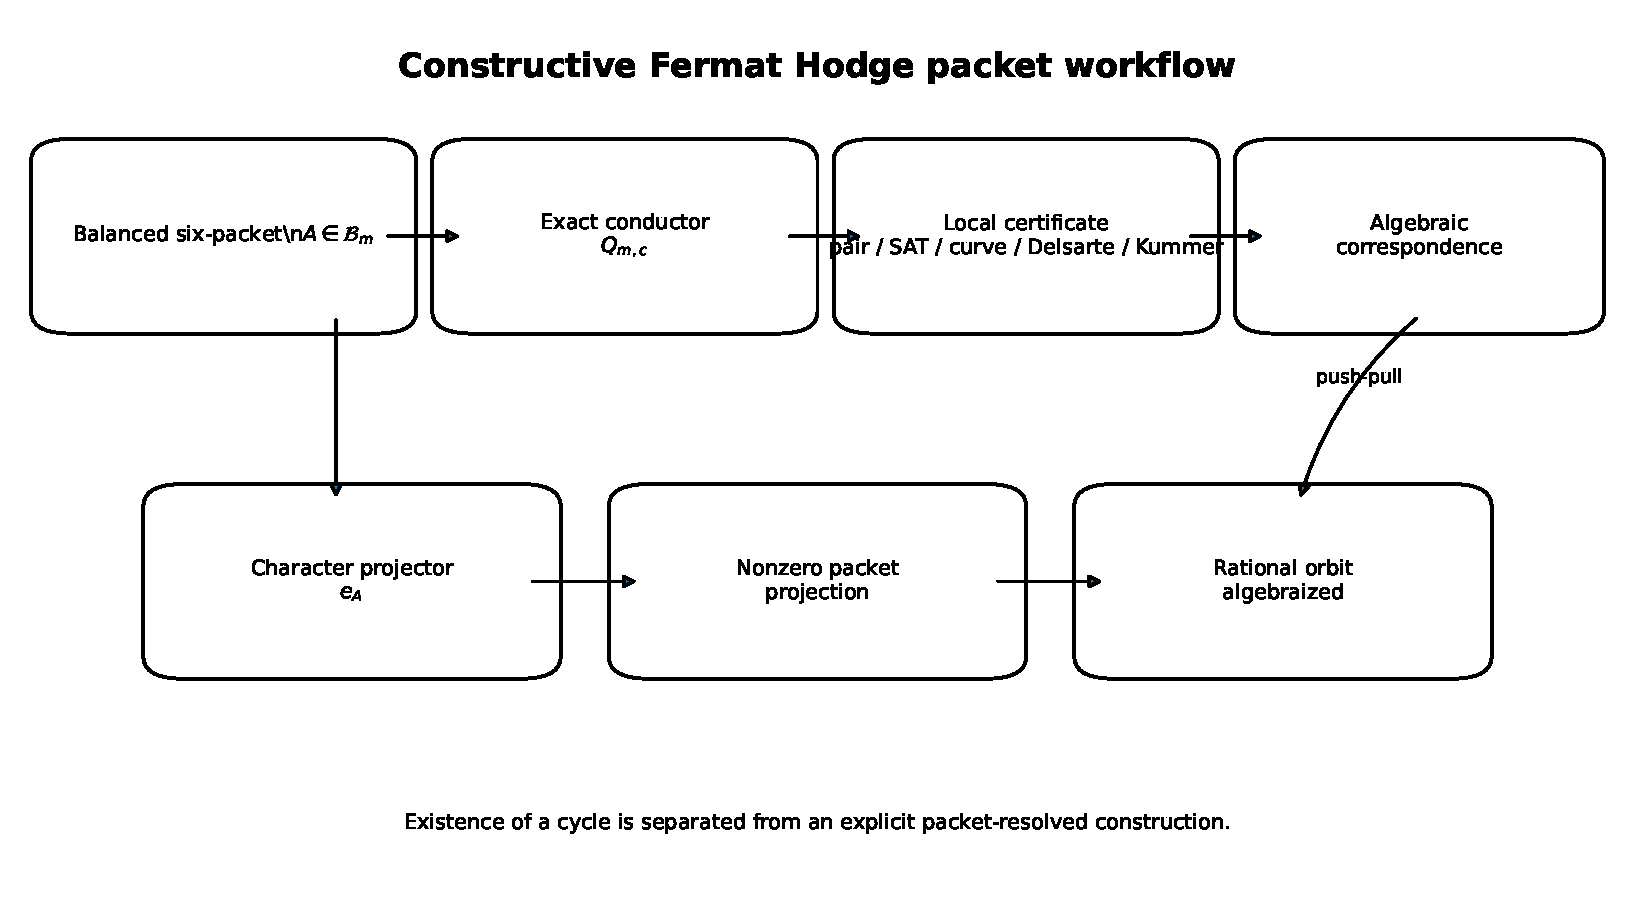
\includegraphics[width=0.94\textwidth]{33_fermat_packet_pipeline.pdf}
\caption{A constructive packet proof separates finite Hodge classification from the algebraic correspondence that realizes the packet.}
\end{figure}

\section{Centered Fourier form}
Define
\[
\rho_m(r)=\langle r\rangle_m-\frac m2,
\qquad
F_a(u)=\sum_i\rho_m(ua_i).
\]
Then \(a\) is balanced if and only if \(F_a(u)=0\) for all units. Moreover,
\[
F_a(-u)=-F_a(u),
\]
so only odd characters occur. For a Dirichlet character \(\chi\) on \(U_m\), put
\[
\mathcal B_{m,\chi}(r)=
\sum_{u\in U_m}\rho_m(ur)\overline{\chi(u)}.
\]
Finite Fourier inversion gives the exact criterion
\[
\boxed{
 a\in\mathcal B_m
 \Longleftrightarrow
 \sum_i\mathcal B_{m,\chi}(a_i)=0
 \quad\text{for every odd }\chi.
}
\tag{7.3}
\]
This formulation is the basis for the prime-power classification and the conductor-defect tree.

\chapter{Exact conductor polyphase}
For a packet \(a\), define
\[
g(a)=\gcd(m,a_0,\ldots,a_5),
\qquad
c(a)=\frac{m}{g(a)}.
\]
Writing \(a=g(a)b\), the coordinate-power map
\[
\pi_{g(a)}:X_m^4\longrightarrow X_{c(a)}^4,
\qquad [x_i]\longmapsto[x_i^{g(a)}],
\]
sends the degree-\(c(a)\) character packet \(b\) to the degree-\(m\) packet \(a\).

\begin{theorem}[Conductor descent]
Every imprimitive balanced packet at degree \(m\) is the coordinate-power pullback of a unique full-conductor packet at its exact conductor \(c\mid m\). Consequently
\[
\mathcal B_m=\bigsqcup_{c\mid m}L_{m/c}\mathcal B_c^{\mathrm{full}}.
\]
\end{theorem}
\begin{proof}
If every occupied residue is divisible by \(g\), divide the six entries and the modulus by \(g\). Since
\[
\langle ugb_i\rangle_{gc}=g\langle \bar u b_i\rangle_c,
\]
the balance equation descends. The maximal common divisor is unique. The converse follows by scaling.
\end{proof}

For \(d\mid m\), let
\[
E_{m,d}=\frac1{(m/d)^5}\pi_{m/d}^*\pi_{m/d*}.
\]
On a character of exact conductor \(c\),
\[
E_{m,d}=\begin{cases}1,&c\mid d,\\0,&c\nmid d.\end{cases}
\]
Therefore
\[
\boxed{E_{m,d}E_{m,e}=E_{m,\gcd(d,e)}.}
\tag{8.1}
\]
M"obius inversion produces pairwise orthogonal exact-conductor projectors
\[
\boxed{
Q_{m,c}=\sum_{d\mid c}\mu(c/d)E_{m,d}.
}
\tag{8.2}
\]
They satisfy
\[
Q_{m,c}Q_{m,e}=\delta_{ce}Q_{m,c},
\qquad
\sum_{c\mid m}Q_{m,c}=I.
\]
Hence
\[
\boxed{
H^4_{\mathrm{prim}}(X_m^4,\Q)
=\bigoplus_{c\mid m}\operatorname{im}Q_{m,c}.
}
\tag{8.3}
\]
Each \(Q_{m,c}\) is a rational linear combination of graph correspondences, so the conductor decomposition is itself algebraic.

\begin{figure}[htbp]
\centering
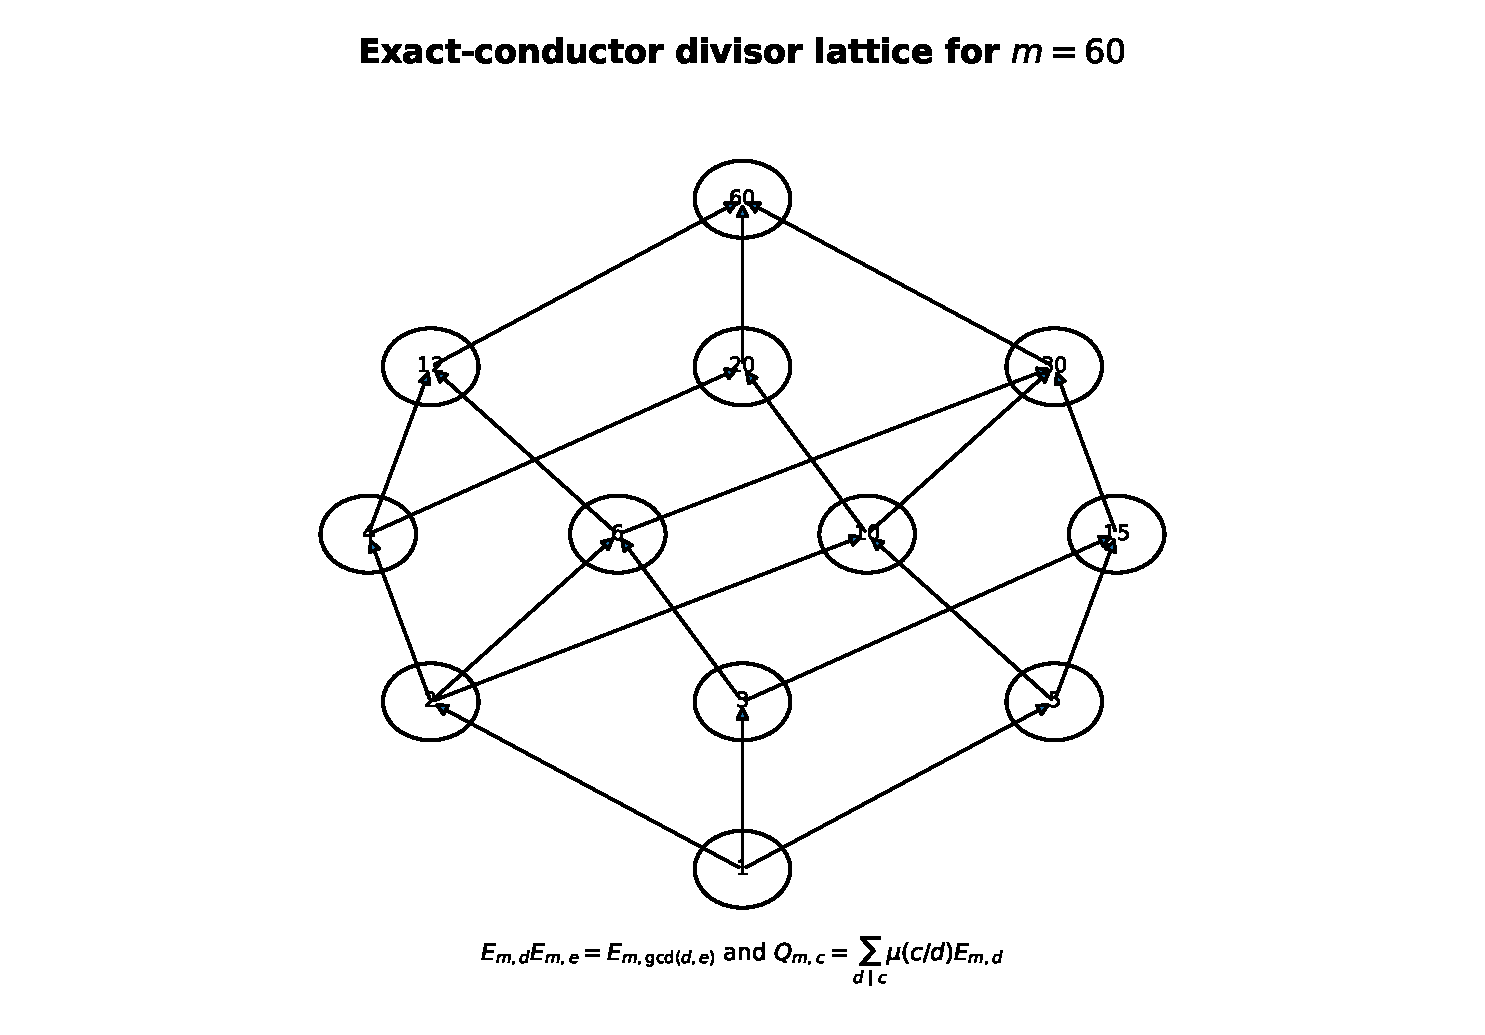
\includegraphics[width=0.82\textwidth]{34_conductor_divisor_lattice.pdf}
\caption{The divisor lattice is the correct all-degree progression. Only full-conductor seeds require new analysis.}
\end{figure}

\chapter{Algebraic certificate grammar}
Fix a full-conductor orbit in \(\mathcal B_m\). The constructive program tests a hierarchy of increasingly general certificate channels.

\section{Complementary pairs}
For \(1\le r<m\), let
\[
p_r=e_r+e_{m-r}.
\]
A packet is pair-decomposable when
\[
n=p_{r_1}+p_{r_2}+p_{r_3}.
\tag{9.1}
\]
These are the standard linear-cycle or Tate-pair packets.

\section{Balanced four-packets and saturation}
Let
\[
\mathcal F_m=
\left\{
\gamma\in\mathbf N^{m-1}:
\mathbf1^T\gamma=4,
\quad R_m\gamma=2m\,\mathbf1
\right\}.
\]
A saturated certificate is an exact nonnegative identity
\[
\boxed{
 n+\sum_{j=1}^{2N-3}p_{r_j}
 =\sum_{i=1}^N\gamma_i,
 \qquad \gamma_i\in\mathcal F_m.
}
\tag{9.2}
\]
The case \(N=2\) is one-step quasi-decomposition. Higher \(N\) allows several surface packets to reconstruct one six-packet after Tate stabilization.

Under the standard associative Fermat join formalism, (9.2) yields an isomorphism of character motives after tensoring with Tate factors. Since the right side is built from algebraic classes on Fermat surfaces, Tate cancellation returns algebraicity of the original packet. The exact Chow-level associativity and cancellation maps should be written explicitly in a final formal treatment.

\section{Dual charges}
An antisymmetric charge is a rational function \(w\) on residues satisfying
\[
w(m-r)=-w(r)
\]
and
\[
\sum_{r\in\gamma}w(r)=0
\qquad\forall \gamma\in\mathcal F_m.
\]
Such a charge vanishes on every complementary pair and on every saturated identity. If \(w(n)\ne0\), the entire lower-packet saturation semigroup is excluded. This is a universal obstruction to a grammar, not a nonalgebraicity theorem.

\section{Curve, Delsarte, and incidence channels}
A curve certificate splits the six entries into triples
\[
a=A\sqcup B,
\qquad \sum A=m,
\quad \sum B=2m,
\quad B=uA\pmod m.
\]
The resulting \((1,1)\) class on a product of Fermat curves is algebraic by Lefschetz \((1,1)\), and the join correspondence returns a surface class.

A Delsarte certificate consists of an exponent matrix and a resolved monomial map to a lower-degree hypersurface carrying an already algebraic packet. An incidence certificate uses algebraic lowering maps
\[
A_r:V\to H^2(Y_r)
\]
whose combined positive transfer
\[
T=\sum_rA_r^\dagger A_r
\]
is invertible on the packet. Divisor lowering and Cayley--Hamilton reconstruction then produce the cycle.

\chapter{The degree-33 rejection branch and its collapse}
The degree-33 Fermat fourfold provided a stringent test because one rational orbit escaped the ordinary decomposable and standard channels. A rejection attempt first isolated the packet, excluded several obvious cycle families, and then discovered a cross-family cubic correspondence that algebraizes it.

\section{The exceptional packet}
A representative is
\[
a=(7,10,13,19,22,28),
\]
or after permutation,
\[
\widetilde a=(7,19,28,10,13,22).
\]
Every unit conjugate has residue sum \(99=3\cdot33\), so the orbit is rational of type \((2,2)\). It is not totally pair-decomposable. The previously proposed symmetric surface
\[
W=\{p_1(x^{11})=p_2(x^{11})=p_3(x^{11})=0\}
\]
does not carry the primitive packet: Newton's identity makes the third equation redundant on \(X_{33}^4\), and
\[
[W]=242h^2.
\]
Thus \(W\) is purely ambient.

\section{Klein--Delsarte cubic}
Consider the smooth cubic fourfold
\[
Y:\quad y_0^2y_4+y_1^2y_0+y_2^2y_1+y_3^2y_2+y_4^2y_3+y_5^3=0.
\]
An explicit monomial exponent matrix gives a dominant rational map
\[
\phi:X_{33}^4\dashrightarrow Y
\]
whose projective-torus lattice map has Smith diagonal
\[
(1,33,33,33,33),
\]
so the generic torus degree is \(33^4\).

Take the cubic Jacobian-ring class
\[
P(y)=y_1y_2y_5.
\]
It is nonzero in the degree-three Jacobian ring. The residue pullback has the exact exponent identity
\[
C^Tb+10\mathbf1=(6,18,27,9,12,21)=\widetilde a-\mathbf1.
\tag{10.1}
\]
Therefore the pullback of the corresponding primitive cubic \((2,2)\)-class lies in the one-dimensional Fermat line \(V(\widetilde a)\).

Because the graph is defined over \(\Q\), its image is Galois-stable. Containing one character line forces it to contain the complete rational orbit. Rational \((2,2)\) classes on the cubic are algebraized through its Fano variety of lines, and the graph correspondence transports those cycles back to the Fermat fourfold.

\begin{theorem}[Degree-33 packet closure]
The rational packet generated by \((7,10,13,19,22,28)\) is algebraic on \(X_{33}^4\).
\end{theorem}

\begin{figure}[htbp]
\centering
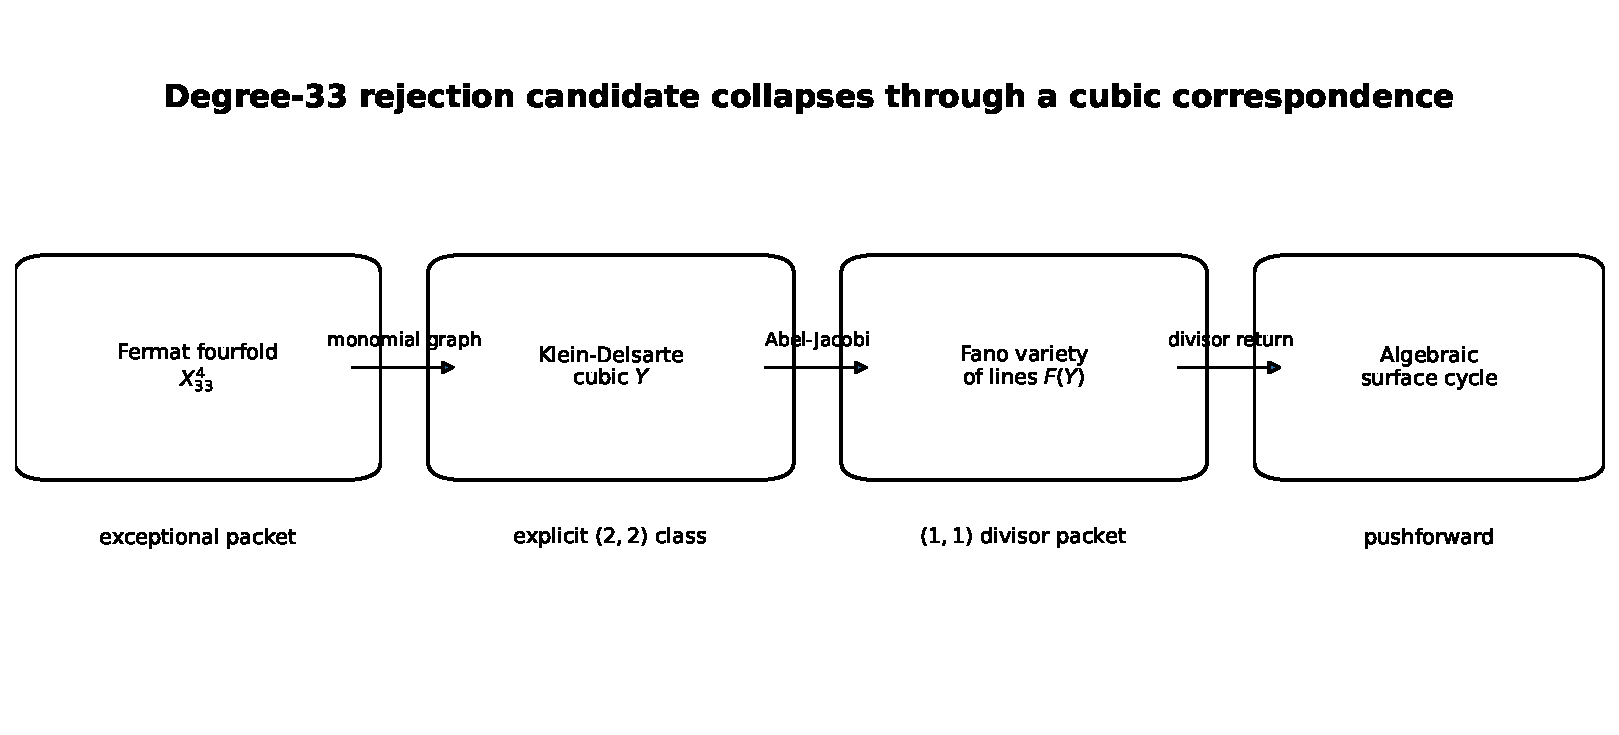
\includegraphics[width=0.94\textwidth]{35_degree33_klein_correspondence.pdf}
\caption{The exceptional degree-33 packet is reached through a lower-degree cubic and a divisor-lowering incidence correspondence.}
\end{figure}

The episode is methodologically important. Failure of a finite cycle grammar is not evidence of nonalgebraicity. It may indicate a missing cross-family correspondence.

\chapter{Infinite towers and full-conductor promotion}
The coordinate-power maps propagate every solved seed through infinitely many degrees.

\begin{theorem}[Infinite packet tower]
Let \(W\) be an algebraic rational character packet on \(X_d^{2p}\). For every \(k\ge1\), its coordinate-power pullback is an algebraic packet on \(X_{kd}^{2p}\). In particular, the degree-33 exceptional packet yields a 20-dimensional algebraic packet on every \(X_{33k}^4\).
\end{theorem}

The tower packet remains an old conductor-33 sector. A stronger construction appends a complementary pair
\[
(1,m-1)
\]
after scaling a solved seed to modulus \(m=kd\). If
\[
b=(b_0,\ldots,b_{2p+1})
\]
is algebraic at degree \(d\), then
\[
\Theta_{m,b}=(kb_0,\ldots,kb_{2p+1},1,m-1)
\]
has full raw conductor \(m\) and middle Hodge type two dimensions higher. Its rational orbit has dimension \(\varphi(m)\). This produces full-raw-conductor algebraic packets of unbounded rank.

Raw conductor is not the complete novelty invariant: removing Tate pairs or reversing joins can reveal a smaller stable conductor. The stable residual should therefore be defined only after eliminating conductor descent, Tate suspension, joins, Delsarte pullbacks, and incidence channels.

\chapter{Prime-power classification}
The odd prime-power classification follows from a primitive-character filtration and a six-entry mass bound.

\section{Valuation strata and orbit mass}
Let \(m=p^r\) with \(p\) odd. Decompose the entries by exact \(p\)-adic valuation. At one stratum, write \(a=p^jb\), with \(b\in U_{p^{r-j}}\), and define the odd count
\[
\delta_j(b)=n_j(b)-n_j(-b).
\]
Since the packet has six entries,
\[
\|\delta_j\|_1\le 12.
\tag{12.1}
\]
Primitive odd characters force \(\delta_j\) to be constant on the kernel cosets of
\[
U_{p^s}\to U_{p^{s-1}}.
\]
A nonzero odd kernel-orbit defect has mass at least \(2p\).

\section{Large odd primes}
If \(p\ge7\), then \(2p>12\), so every odd defect vanishes. Each residue occurs with the same multiplicity as its complement. Therefore every packet is three complementary pairs.

\section{The three-primary branch}
At \(p=3\), a kernel orbit has three elements. Define
\[
O_b=\{b,b+q,b+2q\},
\qquad q=3^{r-1},
\]
and
\[
\Gamma_b=O_b\sqcup\{3(q-b)\}.
\]
The packet \(\Gamma_b\) is a balanced four-packet. A case analysis on the number of oriented kernel orbits gives exact identities expressing every full-conductor nonpair packet as a pair/surface packet or a one-step saturated sum of two balanced four-packets.

\section{The five-primary branch}
At \(p=5\), a nonzero odd defect consumes exactly five unit entries. The sixth entry is forced by balance. Up to the unit action there is one full-conductor exceptional orbit
\[
\boxed{
\alpha_{5^r}=
(1,1+q,1+2q,1+3q,1+4q,5q-5),
\qquad q=5^{r-1}.
}
\tag{12.2}
\]
All other packets lie in the pair/surface grammar. The family (12.2) is the pure five-primary Hasse--Davenport branch.

\begin{figure}[htbp]
\centering
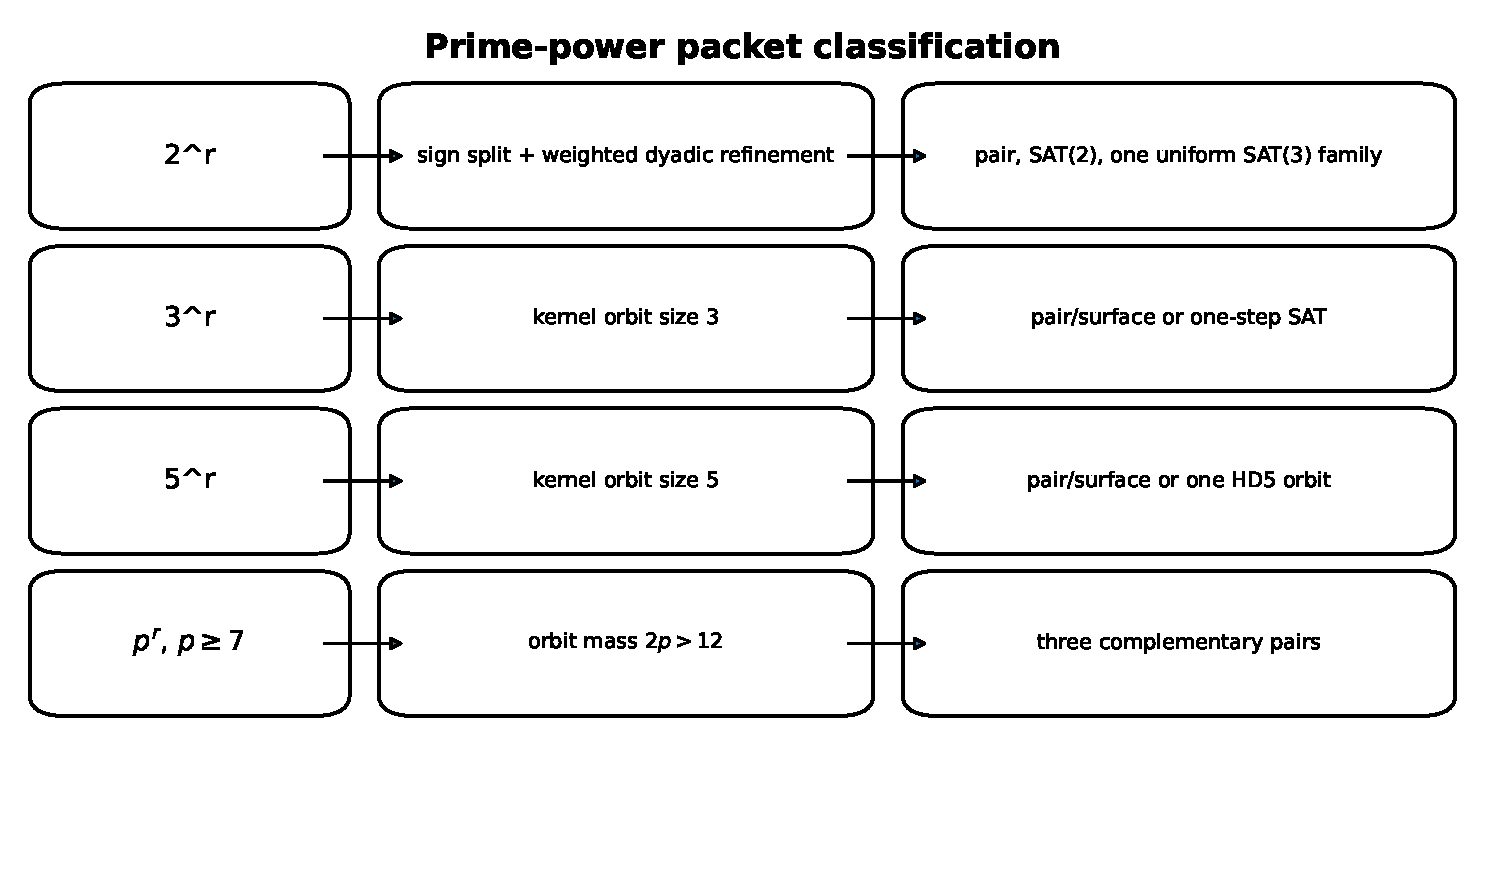
\includegraphics[width=0.91\textwidth]{36_prime_power_classification.pdf}
\caption{The six-entry mass bound produces a complete odd prime-power classification and isolates the five-primary family.}
\end{figure}

\begin{center}
\begin{tabular}{rrrr}\toprule $m$ & Full orbits & Pair/SAT(2) & Residual \\
\midrule
49 & 124 & 124 & 0 \\
81 & 436 & 436 & 0 \\
125 & 827 & 826 pair & 1 \\
\bottomrule\end{tabular}

\end{center}

\chapter{Weighted dyadic reconstruction}
Prime \(2\) cannot be handled by inserting \(p=2\) into the odd-prime orbit-mass proof. The unit group has the separate form
\[
\mathbf Z_2^\times\cong\{\pm1\}\times(1+4\mathbf Z_2).
\]
The first address is a sign packet; only afterward does the principal-unit refinement begin.

Let \(m=2^s\) and \(h=2^{s-1}\). For an odd residue \(b\pmod h\), its two lifts are \(b\) and \(b+h\). Define
\[
L_sn(b)=n(b)+n(b+h),
\qquad
D_sn(b)=n(b)-n(b+h).
\]
For every odd unit \(u\), one has the exact weighted identity
\[
\boxed{
\begin{aligned}
&n(b)\rho_s(ub)+n(b+h)\rho_s(u(b+h))\\
&\qquad=L_sn(b)\rho_{s-1}(\bar ub)
+2^{s-2}D_sn(b)\varepsilon_s(u,b),
\end{aligned}
}
\tag{13.1}
\]
where \(\varepsilon_s(u,b)\in\{\pm1\}\). Repetition yields a Haar-like expansion whose detail packets carry visible powers of two. The Hodge balance equation becomes a binary carry relation between weighted details.

\begin{figure}[htbp]
\centering
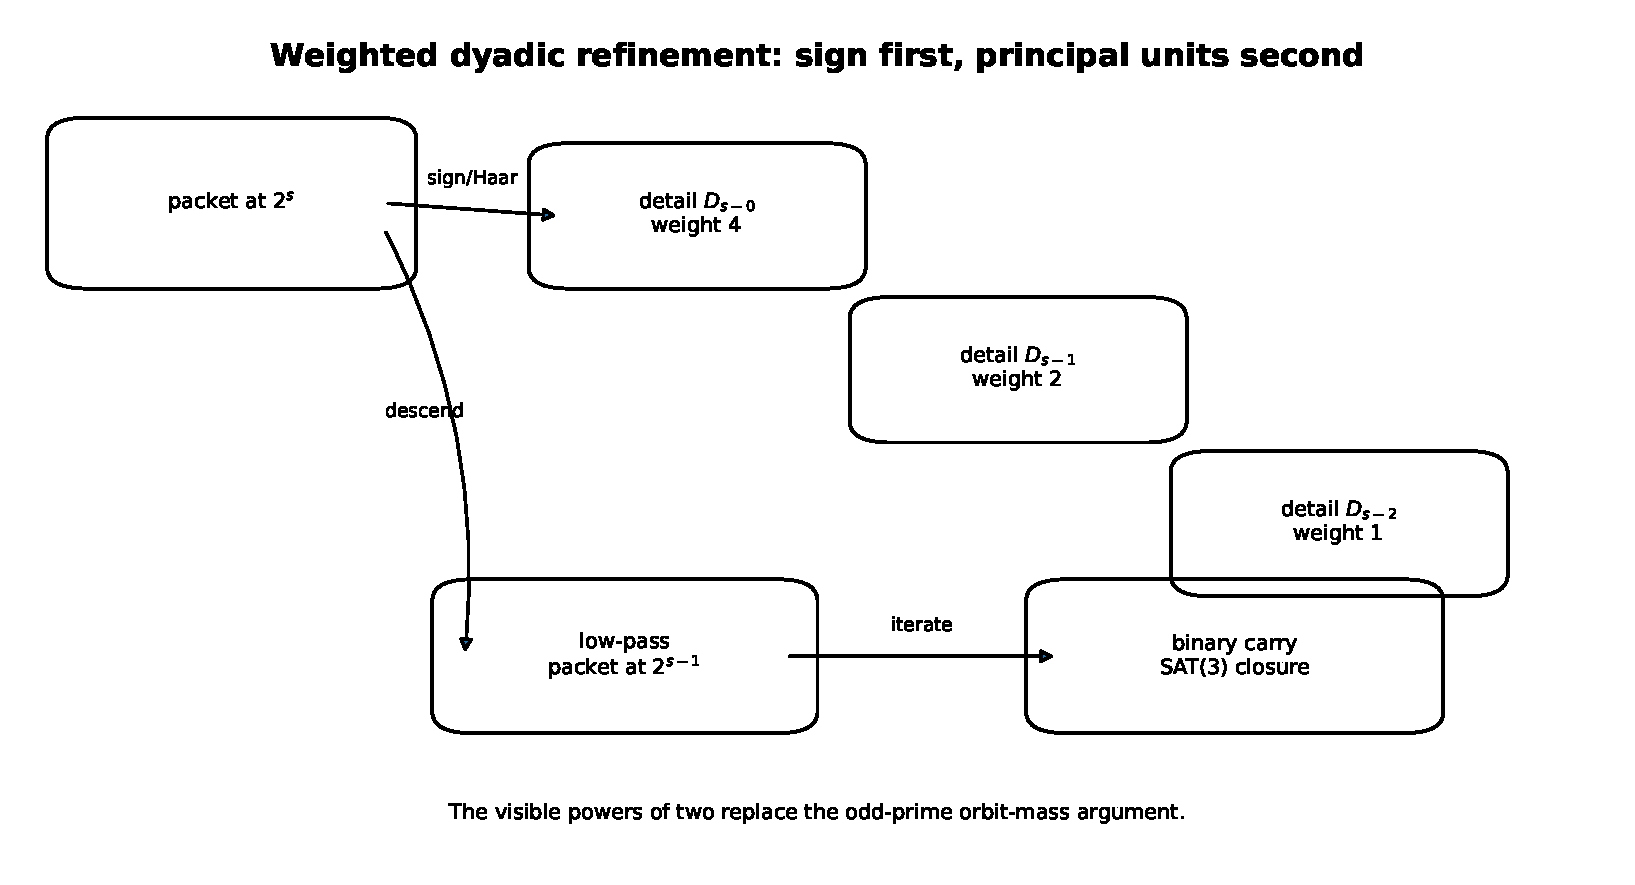
\includegraphics[width=0.90\textwidth]{37_dyadic_weighted_refinement.pdf}
\caption{At prime two, sign refinement and powers-of-two weights motivate the exact defect tree used in the all-degree classification.}
\end{figure}

Exact enumeration gives:
\begin{center}
\begin{tabular}{rrrrrr}\toprule $m$ & Full orbits & Pair & SAT(2) & SAT(3) & Unresolved \\
\midrule
8 & 13 & 9 & 4 & 0 & 0 \\
16 & 45 & 27 & 18 & 0 & 0 \\
32 & 134 & 91 & 42 & 1 & 0 \\
64 & 419 & 331 & 87 & 1 & 0 \\
128 & 1435 & 1259 & 175 & 1 & 0 \\
\bottomrule\end{tabular}

\end{center}
The table suggests one residual orbit beginning at \(m=32\). The remainder of this chapter proves that this orbit is the only one in every dyadic degree.

\section{Complement defects and dyadic triangles}
Put
\[
q=\frac m4,
\qquad h=2q,
\qquad m=4q.
\]
For a packet count vector \(n\), define its oriented complement defect
\[
\partial n=\sum_{r=1}^{h-1}d_n(r)[r],
\qquad
d_n(r)=n_r-n_{m-r}.
\]
The self-complementary residue \(h\) contributes zero. Since
\(\rho_m(m-r)=-\rho_m(r)\), the balanced-packet equation is equivalent to
\[
\sum_{r=1}^{h-1}d_n(r)\rho_m(ur)=0
\qquad\text{for every odd unit }u.
\]
Moreover,
\[
\|\partial n\|_1=\sum_{r=1}^{h-1}|d_n(r)|\le 6.
\]
Thus the dyadic problem is a short-vector problem in an integral defect lattice.

For \(1\le b<q\), define the triangle defect
\[
\kappa_b=[2b]-[b]+[h-b].
\]
It is realized by the four-packet
\[
\Gamma_b=(2b,h-b,h,m-b).
\]

\begin{lemma}[Dyadic triangle relation]
For every odd unit \(u\) and every \(1\le b<q\),
\[
\rho_m(2ub)-\rho_m(ub)+\rho_m(u(h-b))=0.
\]
Consequently \(\kappa_b\) is balanced and \(\Gamma_b\in\mathcal F_m\).
\end{lemma}
\begin{proof}
Let \(x=\langle ub\rangle_m\). If \(0<x<h\), then
\[
\rho_m(2x)=2x-h,
\qquad
\rho_m(x)=x-h,
\qquad
\rho_m(h-x)=-x.
\]
Their indicated combination is zero. If \(h<x<m\), write \(x=m-y\) with \(0<y<h\); then
\[
\rho_m(2x)=h-2y,
\qquad
\rho_m(x)=h-y,
\qquad
\rho_m(h-x)=y,
\]
and the same cancellation occurs. Since \(u\) is odd, \(uh\equiv h\pmod m\), so \(u(h-b)\equiv h-ub\pmod m\). This proves the identity.
\end{proof}

\section{The integral triangle basis}
Let
\[
\mathcal K_m=
\left\{
 d\in\mathbf Z^{h-1}:
 \sum_{r=1}^{h-1}d(r)\rho_m(ur)=0
 \text{ for every odd }u
\right\}.
\]
The triangle relations do not merely generate examples; they form the whole balanced defect lattice.

\begin{theorem}[Integral dyadic triangle basis]
For \(m=2^s\), \(s\ge3\), the vectors
\[
\{\kappa_b:1\le b<q\}
\]
form a \(\mathbf Z\)-basis of \(\mathcal K_m\).
\end{theorem}
\begin{proof}
Set \(r_0=q/2\). On the vertex set
\[
V_m=\{1,2,\ldots,q-1\},
\]
define, for \(b\ne r_0\),
\[
p(b)=
\begin{cases}
2b,&b<r_0,\\
2(q-b),&b>r_0,
\end{cases}
\qquad
\epsilon_b=
\begin{cases}
+1,&b<r_0,\\
-1,&b>r_0.
\end{cases}
\]
The map \(p\) raises the two-adic valuation by one, so repeated application reaches \(r_0\). It therefore defines a rooted tree.

Suppose \(d=\sum_{b=1}^{q-1}z_b\kappa_b\). Its even coordinates are
\[
d(q)=z_{r_0},
\qquad
d(2b)=z_b-\epsilon_bz_{p(b)}
\quad(b\ne r_0).
\]
Starting at the root and moving toward the leaves, these equations recover every \(z_b\) integrally. Hence the triangle vectors are linearly independent and their even-coordinate map is unimodular.

Now take \(d\in\mathcal K_m\), recover the unique integers \(z_b\) from its even coordinates, and subtract \(\sum_bz_b\kappa_b\). The residual balanced vector is supported only on the odd residues \(1\le r<h\). The corresponding square sawtooth matrix is nonsingular. Indeed, extend an odd-support vector to an odd function on \(U_m\). Convolution with \(\rho_m\) is diagonalized by the odd Dirichlet characters, with eigenvalues
\[
\lambda_\chi=
\sum_{a\in U_m}\rho_m(a)\overline{\chi(a)}
=
\sum_{a\in U_m}a\overline{\chi(a)}.
\]
If \(\chi\) is induced from a primitive odd character \(\chi^*\) of conductor \(2^t\), then
\[
\lambda_{\chi,2^s}=2^{s-t}\lambda_{\chi^*,2^t}.
\]
The primitive value is, up to a nonzero scalar, the generalized Bernoulli value \(B_{1,\overline{\chi^*}}\), equivalently \(-L(0,\overline{\chi^*})\), and is nonzero for every odd primitive character \cite{WashingtonCyclotomic}. Thus every odd Fourier eigenvalue is nonzero. The odd residual must vanish, so the \(\kappa_b\) span \(\mathcal K_m\) over \(\mathbf Z\).
\end{proof}

\section{The trivalent defect tree}
The integral basis turns defect mass into exact tree variation. Define a sign gauge by
\[
\tau_{r_0}=1,
\qquad
\tau_b=\epsilon_b\tau_{p(b)},
\qquad
y_b=\tau_bz_b.
\]
Attach one zero-valued boundary leaf to the root and two zero-valued boundary leaves to every odd vertex. Every vertex of the resulting augmented tree \(\widetilde T_m\) has degree three. The boundary edges correspond bijectively to defect coordinates: the root edge is labelled \(q\), the edge from \(b\) to \(p(b)\) is labelled \(2b\), and the two leaves at an odd \(b\) are labelled \(b\) and \(h-b\).

\begin{theorem}[Exact trivalent-tree norm]
If \(d=\sum_bz_b\kappa_b\in\mathcal K_m\), then
\[
\boxed{
\|d\|_1
=|y_{r_0}|
+\sum_{b\ne r_0}|y_b-y_{p(b)}|
+2\sum_{\substack{1\le b<q\\ b\text{ odd}}}|y_b|.
}
\tag{13.2}
\]
The right side is the total variation of the integer function \(y\) on \(\widetilde T_m\) with zero boundary values.
\end{theorem}
\begin{proof}
The root coordinate is \(d(q)=z_{r_0}\). For \(b\ne r_0\), multiplying
\(d(2b)=z_b-\epsilon_bz_{p(b)}\) by \(\tau_b\) gives
\[
\tau_bd(2b)=y_b-y_{p(b)}.
\]
For odd \(b\), the two odd coordinates are
\[
d(b)=-z_b,
\qquad
d(h-b)=z_b.
\]
Taking absolute values and summing all defect coordinates gives (13.2).
\end{proof}

For an integer-valued \(y\), discrete coarea gives
\[
\operatorname{TV}(y)
=
\sum_{k\ge1}|\partial\{y\ge k\}|
+
\sum_{k\ge1}|\partial\{y\le-k\}|.
\tag{13.3}
\]
If \(S\) is a finite forest of internal vertices of a trivalent tree and \(c(S)\) is its number of connected components, then
\[
|\partial S|=|S|+2c(S),
\tag{13.4}
\]
because \(3|S|=2(|S|-c(S))+|\partial S|\).

\begin{proposition}[All defect shapes of mass at most six]
Let \(d\in\mathcal K_m\) satisfy \(\|d\|_1\le6\), and let \(y\) be its gauged coefficient function. Exactly one of the following occurs:
\begin{enumerate}
\item \(y=0\)
\item \(y=\pm2\) at one vertex and is zero elsewhere
\item \(y\) has two singleton components, each with value \(\pm1\)
\item \(y=\pm1\) on one connected subtree containing at most four vertices and is zero elsewhere.
\end{enumerate}
For a balanced four-packet, only the zero shape, a single vertex, or one tree edge can occur.
\end{proposition}
\begin{proof}
Apply (13.3)--(13.4). A nonempty level-set component with \(k\) vertices costs \(k+2\). If \(|y|\ge2\), two nonempty nested level sets already cost at least six; equality forces both to be the same singleton. If positive and negative values both occur, their first level sets cost at least three each; equality forces two singleton components. Otherwise \(y\) has one sign, and a connected support of size \(k\) costs \(k+2\), so \(k\le4\). Two same-sign components can have total cost at most six only when both are singletons. Replacing six by four leaves only a vertex or an edge.
\end{proof}

\section{SAT(2) closure and the four-star obstruction}
For a defect \(d\), let \(\operatorname{red}(d)\) be the unmatched residue multiset: a positive coefficient at \(r\) contributes copies of \(r\), while a negative coefficient contributes copies of \(m-r\). Its length is \(\|d\|_1\). Every packet with defect \(d\) is \(\operatorname{red}(d)\) together with complementary pairs and copies of \(h\).

A one-vertex tree atom has defect \(\pm\kappa_b\) after the gauge sign and is represented by \(\Gamma_b\) or its conjugate; its reduced length is three and its fourth entry is \(h\). A one-edge atom has defect mass four, so its reduced multiset itself is a balanced four-packet. A zero atom is any union of two complementary pairs.

\begin{theorem}[Exact SAT(2) criterion]
Let \(n\) be a balanced six-packet at modulus \(m=2^s\). Then \(n\) is pair-decomposable or has an SAT(2) certificate unless its gauged defect is \(\pm1\) on a four-vertex star \(K_{1,3}\) in the internal tree \(T_m\). A four-star has no SAT(2) certificate.
\end{theorem}
\begin{proof}
Every nonstar shape in the preceding proposition splits into at most two four-packet atoms:
\begin{itemize}
\item a vertex or edge is paired with a zero atom
\item a three-vertex path is an edge plus its remaining terminal vertex
\item a four-vertex path is the union of two disjoint edges
\item a doubled singleton is two copies of one vertex atom
\item two singleton components are the corresponding two vertex atoms.
\end{itemize}
These defect splittings lift to exact nonnegative multiset identities. For a vertex, the neutral remainder of the six-packet is \(h\) plus one complementary pair; for an edge it is one complementary pair. A zero four-packet absorbs that pair and the stabilizing pair. Cutting a three- or four-vertex path produces exactly one oppositely oriented boundary edge, hence exactly one complementary pair in the union of the two atom packets; this is the SAT(2) stabilizer. In the three-vertex case, the vertex atom also supplies the unique neutral \(h\). For two vertex atoms, their two neutral entries are \((h,h)=p_h\). The zero-defect case is already a union of three complementary pairs. Thus in every nonstar case there are \(\gamma_1,\gamma_2\in\mathcal F_m\) and a complementary pair \(p_r\) such that
\[
n+p_r=\gamma_1+\gamma_2.
\]

Conversely, suppose a four-star defect had an SAT(2) certificate. Each balanced four-packet has tree support equal to zero, one vertex, or one edge. The sum of two such supports must produce four nonzero star vertices. Therefore both supports must be disjoint edges covering all four vertices. This would be a perfect matching of \(K_{1,3}\), which does not exist. Hence the star is the unique tree obstruction to SAT(2).
\end{proof}

\section{Conductor of a star and its unique unit orbit}
The tree also determines exactly when the star obstruction has full conductor.

\begin{lemma}[Star conductor]
Let a four-star have center \(c\), and write \(j=v_2(c)\). The gcd of \(m\) with its six packet entries is
\[
2^{j-1}.
\]
Hence a star has full conductor exactly when \(v_2(c)=1\).
\end{lemma}
\begin{proof}
Use the boundary-edge labels of \(\widetilde T_m\). The two children of \(c\) have valuation \(j-1\). The four boundary edges leaving those children have labels of exact valuation \(j-1\): for \(j=1\) they are the odd leaf labels, and for \(j>1\) they are labels \(2b\) coming from grandchildren of valuation \(j-2\). The two boundary edges leaving the parent side have larger valuation. Thus every nonzero defect coordinate is divisible by \(2^{j-1}\), and at least four have exact valuation \(j-1\). Replacing a defect coordinate \(r\) by the packet entry \(m-r\) does not change its two-adic valuation. The stated gcd follows.
\end{proof}

Assume now \(s\ge5\) and let a full-conductor star have center \(c=2a\) with \(a\) odd. Up to global conjugation, expanding its four triangle atoms gives the unordered packet
\[
P_a=
(8a,q-a,2q-a,2q-4a,3q-a,4q-a).
\tag{13.5}
\]
The cases \(c<q/2\) and \(c>q/2\) give the same unordered tuple after the internal-edge cancellations. Choose an odd \(u\) satisfying
\[
ua\equiv1\pmod{2q}.
\]
Since \(uq\equiv q\) or \(3q\pmod{4q}\), multiplication by \(u\) sends (13.5) to
\[
P_1=(8,q-1,2q-4,2q-1,3q-1,4q-1).
\]
Its conjugate is
\[
\boxed{
A_m=
\left(
1,\frac m4+1,\frac m2+1,\frac m2+4,
\frac{3m}4+1,m-8
\right).
}
\tag{13.6}
\]
Thus every full-conductor star belongs to one \(U_m\)-orbit.

The packet \(A_m\) obeys the exact uniform SAT(3) identity
\[
\begin{aligned}
&A_m+(2,m-2)+(4,m-4)+(m/2,m/2)\\
&=(1,m/2,m/2+1,m-2)\\
&\quad +(2,m/4+1,3m/4+1,m-4)\\
&\quad +(4,m/2,m/2+4,m-8).
\end{aligned}
\tag{13.7}
\]
The first and third packets on the right have defects \(-\kappa_1\) and \(-\kappa_4\). The middle packet has defect \(-\kappa_2+\kappa_{q-1}\), an edge atom. Hence all three are balanced four-packets, and (13.7) is an identity of multisets.

\begin{theorem}[All-degree dyadic uniqueness]
Let \(m=2^s\), \(s\ge3\). Every full-conductor balanced six-packet is pair-decomposable or SAT(2), except that for \(s\ge5\) there is exactly one residual unit orbit, represented by \(A_m\). This orbit is SAT(3) by (13.7). For \(m=8\) and \(m=16\), no four-star exists and there is no residual orbit.
\end{theorem}
\begin{proof}
The trivalent-tree norm and coarea classification list every defect of mass at most six. The SAT(2) criterion closes every listed shape except a four-star. The star-conductor lemma forces a full-conductor star center to have valuation one, and the calculation (13.5)--(13.6) places all such stars in the single orbit of \(A_m\). The trees for \(m=8\) and \(m=16\) have no internal vertex with three internal neighbors. Finally, (13.7) closes the unique residual orbit at saturation depth three.
\end{proof}

\begin{corollary}[Complete dyadic grammar]
After exact conductor descent, every balanced packet at every dyadic modulus is generated by complementary pairs, SAT(2) surface packets, and coordinate-power pullbacks of the single SAT(3) family \(A_{2^t}\). No second residual dyadic family occurs at any depth.
\end{corollary}

\begin{resultbox}[Dyadic target closed]
The former ``uniform dyadic uniqueness'' assumption is now a theorem. Its proof is independent of the finite search: it uses an integral triangle basis, an exact total-variation model on a trivalent tree, discrete coarea, and the conductor of the unique four-star obstruction.
\end{resultbox}

The companion verifier \path{data/Fermat_Hodge_Dyadic_Uniqueness_VERIFICATION.json} independently reproduces the complete orbit counts through \(m=128\), identifies exactly the three displayed representatives at \(m=32,64,128\), checks the tree/SAT(2) criterion against exhaustive certificate search, and audits the structural identities through \(2^{14}\). These computations corroborate the theorem but are not used in place of its proof.

\chapter{Finite global audit through degree 100}
The finite audit exactly enumerates balanced packets, reduces them by unit orbits, checks pair and SAT(2) certificates, and searches higher saturated identities with \(N\le8\). Every returned identity is rechecked by exact integer arithmetic.

All named verification groups pass:
\begin{center}
\begin{tabular}{lrr}\toprule Suite & Passed & Total \\
\midrule
projector resolved hodge calculus & 18 & 18 \\
fermat33 klein closure & 14 & 14 \\
infinite klein tower & 4 & 4 \\
conductor polyphase & 4 & 4 \\
odd prime power audit & 13 & 13 \\
\midrule Total & 53 & 53 \\
\bottomrule\end{tabular}

\end{center}
The dyadic weighted identity passes \(89{,}478{,}480\) coefficient checks through \(2^{14}\). The exact packet audit is complete through degree \(100\) for the implemented grammar.

After removing the degree-33 Klein channel and the degree-39 curve channel, every remaining post-saturation degree in the audit is divisible by five. This is a powerful localization of the residual grammar, but it is not by itself a universal proof.

\begin{figure}[htbp]
\centering
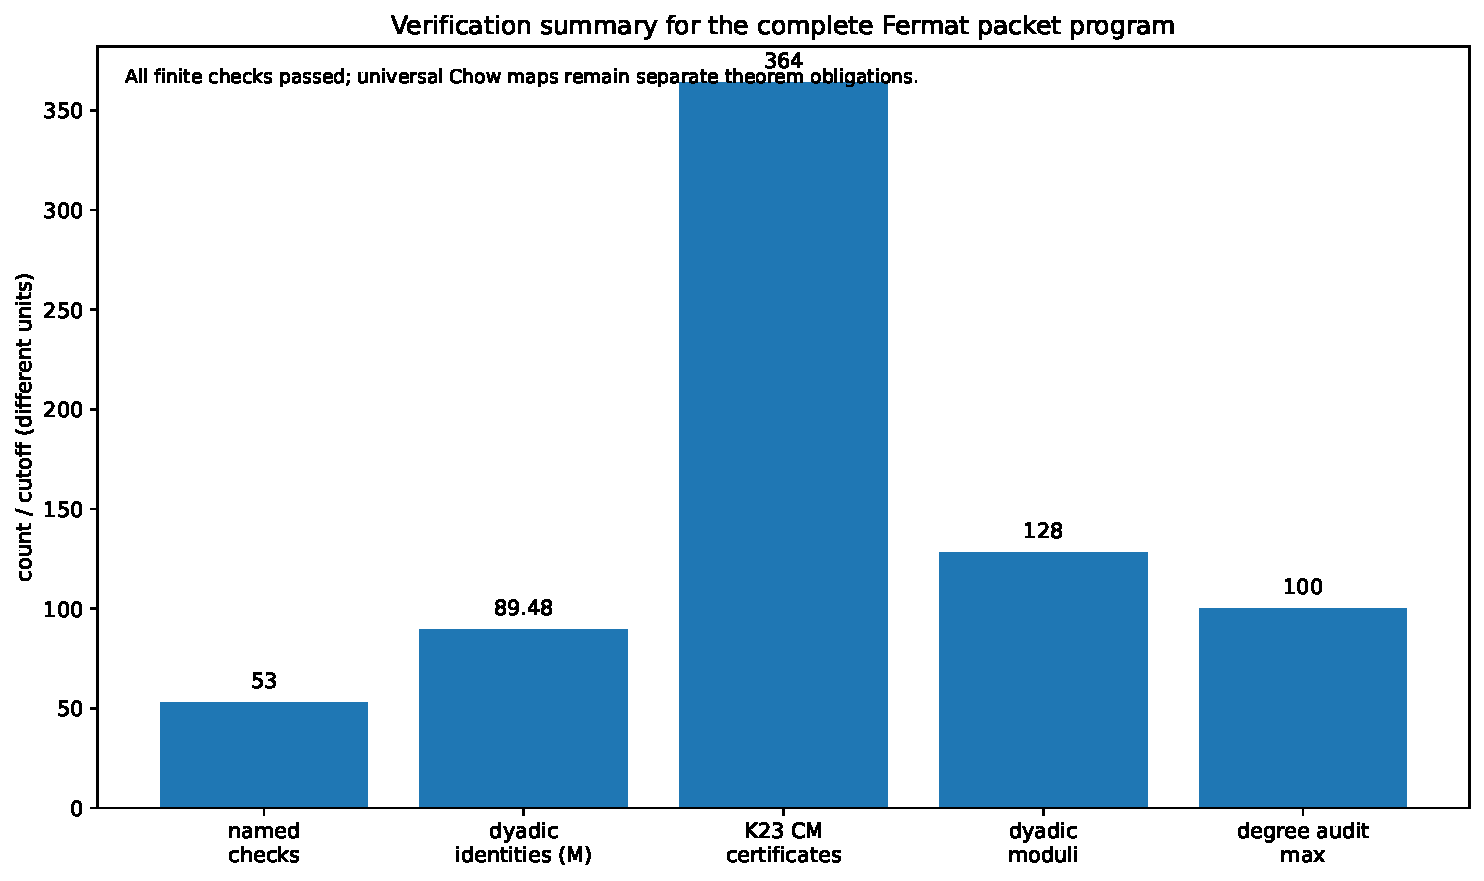
\includegraphics[width=0.82\textwidth]{42_verification_summary.pdf}
\caption{Finite checks validate the symbolic grammar and examples; universal Chow correspondences remain separate theorem obligations.}
\end{figure}

\section{Exact residual representatives}
\small
\begin{longtable}{rp{0.68\textwidth}}\toprule Degree & Post-saturation representatives \\
\midrule\endfirsthead
\toprule Degree & Post-saturation representatives \\
\midrule\endhead
25 & \texttt{(1,6,11,16,20,21)} \\
33 & \texttt{(1,4,16,22,25,31)} \\
35 & \texttt{(1,8,15,22,29,30)} \\
39 & \texttt{(1,7,16,22,34,37)} \\
40 & \texttt{(1,9,17,25,33,35)} \\
45 & \texttt{(1,10,19,28,37,40); (1,19,20,28,30,37)} \\
50 & \texttt{(1,7,27,30,41,44); (1,11,21,31,41,45); (1,13,22,32,40,42)} \\
55 & \texttt{(1,12,23,34,45,50)} \\
65 & \texttt{(1,14,27,40,53,60)} \\
70 & \texttt{(1,6,43,45,57,58); (1,15,29,43,57,65); (1,20,24,42,61,62); (1,20,29,43,57,60); (1,29,35,43,45,57)} \\
75 & \texttt{(1,16,31,46,61,70)} \\
80 & \texttt{(1,17,33,49,65,75)} \\
85 & \texttt{(1,18,35,52,69,80)} \\
90 & \texttt{(1,8,26,62,85,88); (1,19,37,55,73,85); (1,19,37,60,73,80); (1,19,37,65,73,75); (1,23,38,55,74,79); (1,38,46,55,56,74); (2,38,45,55,56,74)} \\
95 & \texttt{(1,20,39,58,77,90)} \\
100 & \texttt{(1,21,41,61,81,95)} \\
\bottomrule\end{longtable}

\normalsize

The residuals are not random. Their mod-5 phase profiles form a small local grammar.

\compactpart{Part VIII. CRT--Kummer Polyphase and the Imaginary CM Half-Twist}

\chapter{Local mod-5 phase grammar}
Assume \(m=5q\) and first suppose \((5,q)=1\). For \(b\pmod q\) and a phase \(r\in\{0,1,2,3,4\}\), let \(\lambda_r(b)\) be the CRT lift satisfying
\[
\lambda_r(b)\equiv r\pmod5,
\qquad
\lambda_r(b)\equiv b\pmod q.
\]
The finite audit reveals four canonical multiplicity profiles, up to multiplication by a unit modulo five:
\[
(1,0,0,0,5),
\quad
(2,1,1,1,1),
\quad
(1,0,2,1,2),
\quad
(1,0,1,3,1).
\]
The first is the complete-five-phase K5 packet, the second is a four-phase K4 lift, and the final two are one K23 pair--triple mechanism.

\begin{figure}[htbp]
\centering
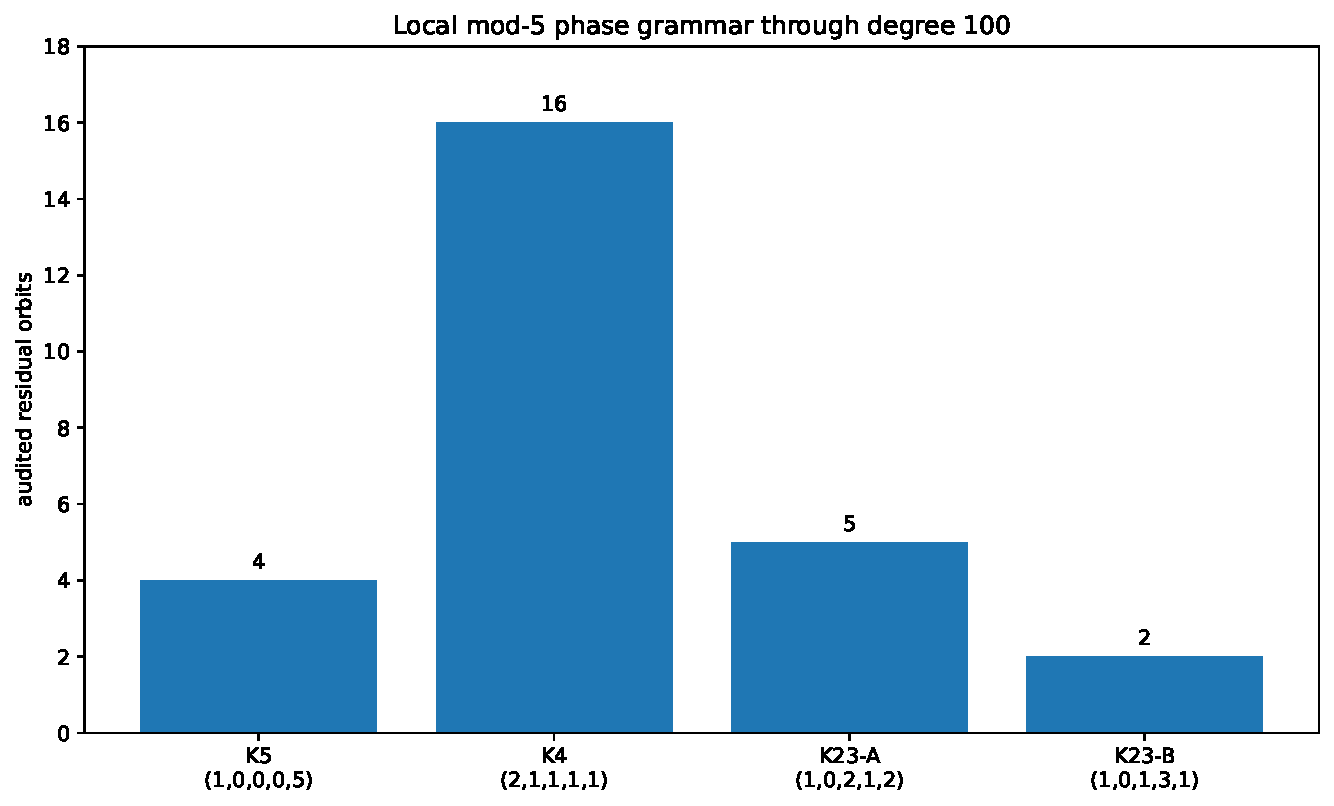
\includegraphics[width=0.76\textwidth]{38_mod5_phase_profiles.pdf}
\caption{Only four local mod-5 profiles occur among the audited residual orbits; the last two unify as K23.}
\end{figure}

\section{K4 four-phase reduction}
Choose nonzero residues \(b,c,d\pmod q\) and put
\[
e\equiv-5^{-1}b\pmod q.
\]
Define
\[
A_{b;c,d}=
(\lambda_1(b),\lambda_2(b),\lambda_3(b),\lambda_4(b),5c,5d)
\]
and
\[
\Gamma_{b;c,d}=(b,c,d,e).
\]

\begin{theorem}[Four-phase CRT reduction]
The six-packet \(A_{b;c,d}\) is balanced modulo \(5q\) if and only if the four-packet \(\Gamma_{b;c,d}\) is balanced modulo \(q\).
\end{theorem}
\begin{proof}
For a unit \(u\), let \(s=\langle ub\rangle_q\) and \(z=\langle u5^{-1}b\rangle_q\). The complete five-element fiber over \(s\) has sum \(5s+10q\); its phase-zero lift is \(5z\). The four nonzero phases therefore sum to \(5s+10q-5z\). Adding the last two entries and imposing the middle value \(15q\) gives
\[
s+\langle uc\rangle_q+\langle ud\rangle_q-z=q.
\]
Since \(\langle ue\rangle_q=q-z\), this is exactly the balance equation for \((b,c,d,e)\).
\end{proof}

All 16 audited K4 residuals reduce exactly to balanced four-packets.

\chapter{K23 pair--triple factorization}
Let a K23 packet have one phase-zero entry and five nonzero phases:
\[
A=P\sqcup T\sqcup\{5e\},
\qquad |P|=2,
\quad |T|=3,
\]
with
\[
\sum P\equiv0\pmod5,
\qquad
\sum T\equiv0\pmod5.
\]
Write
\[
\sum P=5C,
\qquad
\sum T=5D,
\]
and reduce \(C,D\) modulo \(q\) to positive representatives \(c,d\). Define
\[
C_P=P\sqcup\{m-5c\},
\]
\[
S_T=T\sqcup\{m-5d\},
\]
and
\[
L=(5c,5d,5e).
\]

\begin{theorem}[Exact K23 packet identity]
One has the exact multiset equality
\[
\boxed{
A+(5c,m-5c)+(5d,m-5d)=C_P+S_T+L.
}
\tag{15.1}
\]
For every unit \(u\pmod m\),
\[
h_{C_P}(u)+h_{S_T}(u)+h_L(u)=5,
\]
and \(c+d+e\equiv0\pmod q\).
\end{theorem}

The five nonzero phases have only two irreducible possibilities: all five phases are equal, or they contain a complementary pair and a zero-sum triple. Indeed, if no complementary phase pair occurs, the phase support lies in one of four two-element subsets; the zero-sum condition forces all five entries to use one phase. This proves the local K5/K23 dichotomy.

\begin{figure}[htbp]
\centering
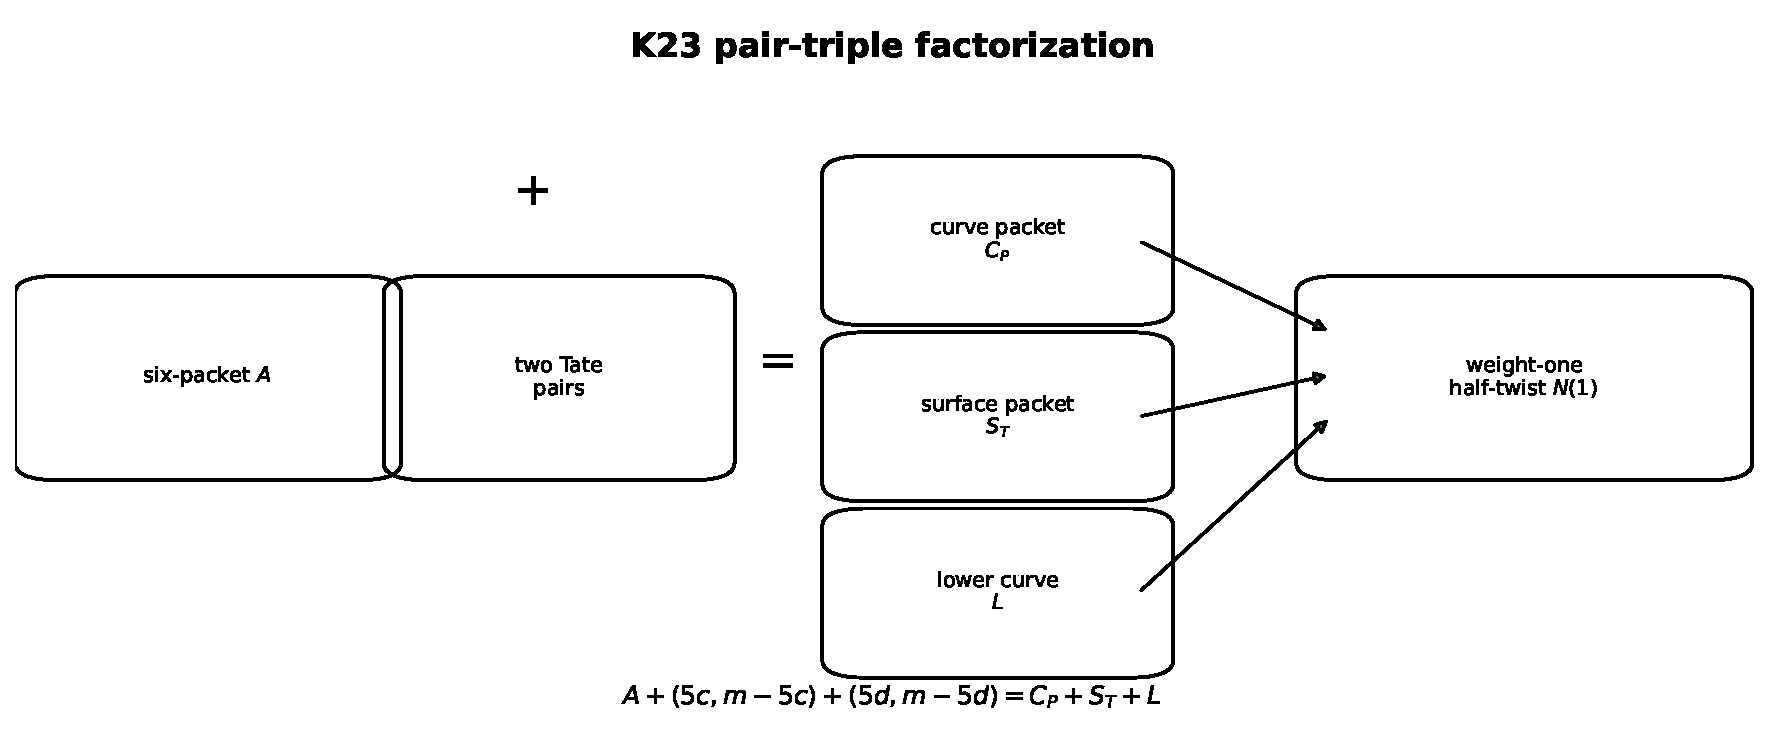
\includegraphics[width=0.94\textwidth]{39_k23_factorization.pdf}
\caption{The K23 packet becomes a curve packet, a surface packet, and a lower curve packet after two explicit Tate-pair stabilizations.}
\end{figure}

At the motive level, write
\[
N=M(C_P)\otimes M(S_T).
\]
The Hodge-level identity implies that \(N(1)\) has weight one and has Hodge type opposite to the lower curve packet \(M(L)\) at every embedding.

\chapter{Imaginary CM selector}
Write the lower curve packet as
\[
\ell=(c,d,e)\pmod q,
\qquad c+d+e\equiv0\pmod q.
\]
Let \(K=\Q(\zeta_q)\) and define
\[
\boxed{
\Delta_\ell=(1-\zeta_q^c)(1-\zeta_q^d)(1-\zeta_q^e).
}
\tag{16.1}
\]

\begin{theorem}[Pure imaginary selector]
\[
\overline{\Delta_\ell}=-\Delta_\ell.
\]
\end{theorem}
\begin{proof}
Since
\[
1-\zeta_q^{-a}=-\zeta_q^{-a}(1-\zeta_q^a),
\]
complex conjugation multiplies the product by
\[
(-1)^3\zeta_q^{-(c+d+e)}=-1.
\]
\end{proof}

For an embedding \(\sigma_u:\zeta_q\mapsto\zeta_q^u\), let
\[
h_\ell(u)=\frac{\langle uc\rangle_q+\langle ud\rangle_q+\langle ue\rangle_q}{q}\in\{1,2\}.
\]
Using
\[
1-e^{2\pi ir/q}=-2i\,e^{\pi ir/q}\sin\frac{\pi r}{q},
\]
one obtains
\[
\sigma_u(\Delta_\ell)
=8i(-1)^{h_\ell(u)}
\prod_{a\in\{c,d,e\}}
\sin\frac{\pi\langle ua\rangle_q}{q}.
\tag{16.2}
\]
Every sine factor is positive, so the sign of the imaginary part is exactly the Hodge sign. Consequently the CM type of \(N(1)\) is the conjugate of the CM type of the lower curve packet:
\[
\boxed{
\Sigma_N=\overline{\Sigma_\ell}.
}
\tag{16.3}
\]
This is the rigorous form of the statement that the half-twist occurs on the imaginary plane.

\begin{figure}[htbp]
\centering
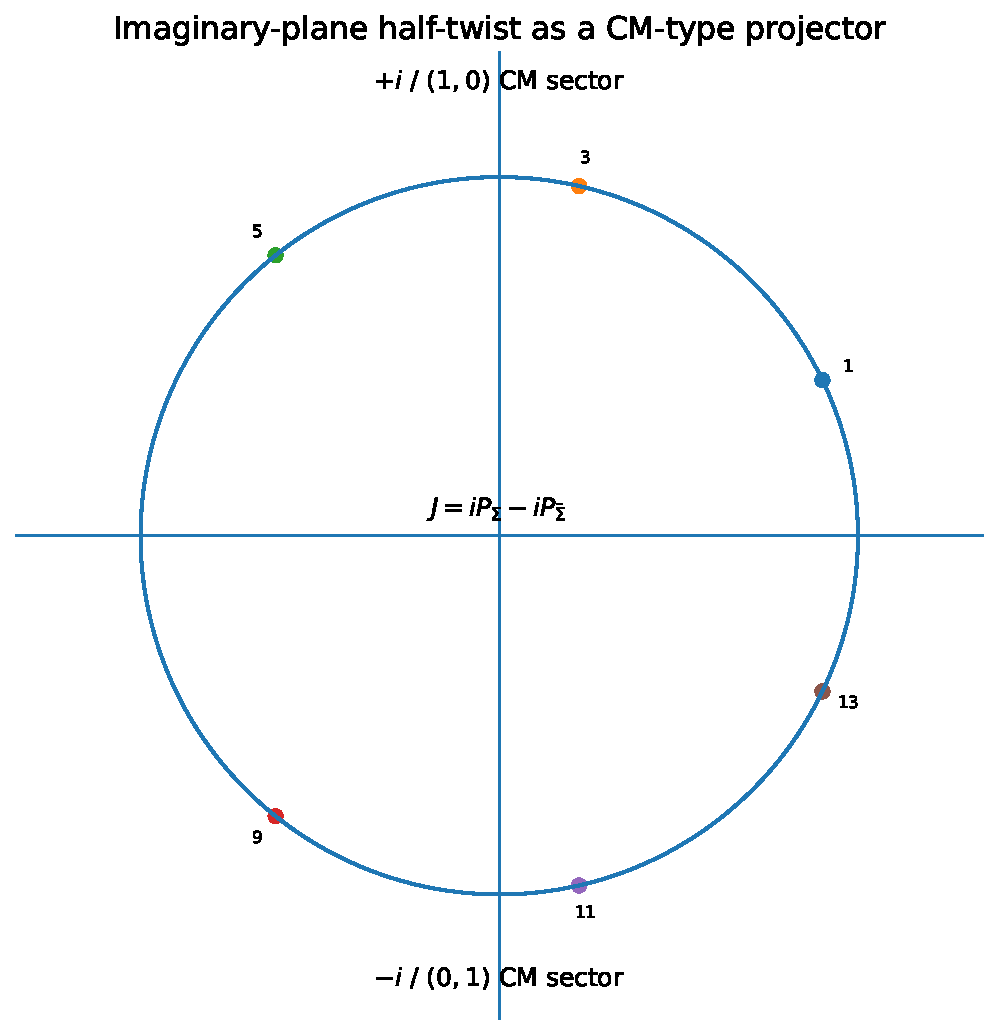
\includegraphics[width=0.73\textwidth]{40_cm_half_plane.pdf}
\caption{The half-twist acts with eigenvalues $+i$ and $-i$ on conjugate CM embedding sectors.}
\end{figure}

The exact audit generates 364 K23 certificates from seven rational packet orbits. Every certificate obeys the opposite curve CM sign, factors through a lower conductor, and is a Galois translate of an upper-half-plane CM type.

\begin{center}
\begin{tabular}{lr}\toprule Item & Value \\
\midrule
K23 rational orbits & 7 \\
Exact K23 certificates & 364 \\
Opposite curve CM sign & True \\
Lower-conductor factorization & True \\
Upper-half-plane CM translate & True \\
\bottomrule\end{tabular}

\end{center}

In the audited cases, the minimal CM conductors are \(3,5,7,\) or \(9\), even when the original fourfold modulus is \(50,70,\) or \(90\). Thus the weight-one carrier is not arbitrary: it is a character factor of the Jacobian of a lower-degree Fermat curve.

\chapter{Explicit carrier and remaining Chow map}
Let \(F_d\) be the Fermat curve of the minimal CM conductor and let \(e_{\Sigma_N}\) be the algebraic character idempotent selecting the required orbit. The explicit carrier is
\[
A_{\Sigma_N}=e_{\Sigma_N}J(F_d)
\]
up to isogeny. The desired constructive theorem is an algebraic correspondence
\[
\Gamma_N\in
\CH^\ast(F_d\times C_P\times S_T)_\Q
\]
inducing
\[
\boxed{
\Gamma_{N*}:
 e_{\Sigma_N}H^1(F_d)
 \xrightarrow{\sim}
 M(C_P)\otimes M(S_T)(1).
}
\tag{17.1}
\]
Once (17.1) is available, its tensor product with the conjugate lower curve packet is a rational \((1,1)\) class on a product of curves or abelian varieties. Lefschetz \((1,1)\) makes it algebraic, and the Shioda--Katsura join maps push the divisor to a codimension-two cycle on \(X_m^4\).

Because the selected character packets are rank one, any nonzero equivariant morphism is an isomorphism. The geometric proof therefore needs only:
\begin{enumerate}
\item a Kummer-convolution or half-twist correspondence with the correct character covariance
\item one nonzero period, Jacobi-sum, or intersection matrix coefficient
\end{enumerate}
The remaining issue is constructive, not a missing Hodge-sign classification. Motivic Gauss and Jacobi sum correspondences, including Davenport--Hasse multiplication in Chow-motive form over finite fields, provide a closely related model \cite{OtsuboYamazaki}, but the characteristic-zero packet map required here is still to be written.

\begin{openproblem}[Explicit CM Packet Correspondence Theorem]
For every K23 packet, construct the correspondence (17.1), pair it with the lower curve packet, and push the resulting divisor through the two Fermat join maps. Prove that the final character projection is nonzero.
\end{openproblem}

\chapter{Correct literature and novelty map}
Kang states a generalized-Hodge theorem for Fermat varieties of dimensions three and four in arbitrary degree \cite{KangFermat}. Separately, da Silva studies which packets are generated by Shioda-style induced-cycle criteria and records the degree-$33$ failure of that criterion \cite{DaSilvaFermat}. These statements are compatible if the latter concerns explicit or restricted constructions rather than abstract existence, but the literature relation should be audited before publication.

The constructive contribution of the packet program is therefore not best described as the first proof of the rational Hodge conjecture for all Fermat fourfolds. Its strongest defensible targets are:
\begin{itemize}
\item explicit conductor projectors as algebraic correspondences
\item an algorithmic packet certificate grammar
\item a worked cross-family Klein--Delsarte construction at degree 33
\item infinite conductor towers and full-raw-conductor promotions
\item odd prime-power packet classifications
\item a weighted dyadic recursion and an all-degree uniqueness theorem with one SAT(3) orbit
\item exact CRT--Kummer reductions for K4 and K23 packets
\item an imaginary CM selector and explicit lower Fermat-curve carriers
\item an explicit packet-resolved Chow correspondence algorithm
\end{itemize}

\begin{resultbox}[Constructive status]
The abstract existence question for Fermat fourfolds is treated as prior published work. The packet program supplies a detailed constructive architecture and several explicit new or potentially new correspondences. The final universal constructive theorem is the explicit CM packet correspondence, not the abstract equality of Hodge and algebraic subspaces.
\end{resultbox}

\compactpart{Part IX. Verification, Audit, and Final Constructive Theorem}

\chapter{Verification ledger}
The complete edition separates symbolic theorems, finite exact checks, geometric correspondences, and literature claims.

\section{Finite checks}
The original Hodge-calculus release passed 18 finite checks. The Fermat extension adds:
\begin{itemize}
\item 14 exact degree-33 Klein checks
\item 4 infinite tower checks
\item 4 exact conductor-polyphase checks
\item 13 odd prime-power checks
\item 89,478,480 dyadic weighted coefficient identities
\item exact packet classifications at dyadic degrees through 128
\item an independent trivalent-tree/SAT(2) audit and structural dyadic checks through $2^{14}$
\item exact balanced-packet audit through degree 100
\item 364 K23 CM-type certificates
\end{itemize}

\section{What finite checks establish}
They establish exact arithmetic identities, matrix products, orbit counts, conductor decompositions, Hodge balance, and nonnegative multiset equalities for every tested instance. They also detect false universal conjectures quickly. The universal dyadic uniqueness statement is not inferred from these checks; it is proved in Chapter 13 by the integral triangle basis and trivalent-tree coarea argument.

\section{What finite checks do not establish}
They do not replace:
\begin{itemize}
\item a universal mixed-prime phase-classification proof beyond the audited range
\item a Chow-level Kummer--Schur or half-twist correspondence
\item a historical priority audit
\end{itemize}

\chapter{Final theorem stack}
The constructive Fermat program can be stated as a dependency stack.

\begin{theorem}[Conditional explicit packet theorem]
Assume the following correspondence statements:
\begin{enumerate}
\item saturated Fermat joins are associative on Chow motives and complementary Tate factors cancel
\item every Delsarte torus map used by the certificate grammar extends through a resolved graph with full-support boundary annihilation
\item every K5, K4, and K23 local phase packet has its prescribed Kummer--Schur or CM half-twist Chow correspondence
\end{enumerate}
Then every rational middle Hodge packet on every Fermat fourfold has an explicit packet-resolved algebraic cycle representative.
\end{theorem}
\begin{proof}
Apply the exact conductor projectors. Descend each nonzero component to its full-conductor seed. Classify the seed by the pair, saturation, curve, Delsarte, dyadic, or Kummer phase grammar. Use the corresponding Chow map to produce a nonzero cycle projection. Pull old packets back to the original degree and sum the orthogonal conductor components. Finally sum the Galois orbit to obtain a rational cycle.
\end{proof}

\begin{openproblem}[Unconditional constructive completion]
Write the missing correspondence maps explicitly and verify their nonzero packet matrix coefficients. The most concentrated target is the rank-one CM map (17.1).
\end{openproblem}

\chapter{Research checklist}
\begin{longtable}{p{0.43\textwidth}p{0.17\textwidth}p{0.32\textwidth}}
\toprule
Task & Status & Required proof object \\
\midrule\endfirsthead
\toprule
Task & Status & Required proof object \\
\midrule\endhead
Universal balanced packet equation & Complete & Finite residue matrix \\
Exact conductor descent & Complete & Coordinate-power graph \\
M"obius conductor projectors & Complete & Rational graph combination \\
Degree-33 Klein packet & Manuscript-level complete & Resolved graph and residue pullback \\
Infinite old-packet towers & Complete & Pullback/pushforward identity \\
Odd prime-power classification & Symbolically complete & Primitive-character filtration \\
Dyadic weighted classification & Complete & Triangle basis, trivalent coarea, star conductor \\
K4 CRT reduction & Complete & Lower balanced four-packet \\
K23 local phase classification & Complete & Pair--triple lemma \\
K23 CM sign descent & Complete & Imaginary selector $\Delta_\ell$ \\
Explicit lower CM carrier & Identified & Fermat-curve character idempotent \\
CM carrier Chow map & Open & Nonzero algebraic correspondence \\
All-degree constructive algorithm & Conditional & Assemble all correspondence channels \\
Historical priority map & Open audit & Compare existence and constructive literature \\
\bottomrule
\end{longtable}

\chapter{Complete-edition conclusion}
The projector-resolved approach transforms the Hodge problem into a hierarchy of exact finite packets and explicit geometric transfers. For arbitrary varieties, the master obstruction remains the Hodge packet not occupied by algebraic-cycle channels. For Fermat fourfolds, diagonal symmetry makes every stage concrete: balanced residue equations, conductor projectors, prime-local refinements, nonnegative packet identities, and rank-one character motives.

The degree-33 rejection attempt illustrates the central lesson. A packet may evade every obvious lower-packet construction and still be algebraic through a hidden cross-family correspondence. The resulting Klein--Delsarte map then seeds infinite conductor towers. The odd prime-power classification and the all-degree dyadic trivalent-tree theorem show that local primes impose distinct packet grammars. The mixed-prime residuals resolve into a finite Kummer phase system. Finally, the imaginary CM selector identifies the precise upper/lower embedding split and reduces the unknown weight-one carrier to a small Fermat-curve Jacobian factor.

The constructive endpoint is now sharply defined:
\begin{resultbox}[Final constructive endpoint]
Construct one nonzero equivariant Chow correspondence between the explicit CM carrier and each remaining packet factor.
\end{resultbox}
This task is narrower than the original conjecture and stronger than a numerical packet classification. It asks for an algorithmic cycle formula that exposes exactly how a Hodge packet becomes algebraic.


\addcontentsline{toc}{part}{Appendices}

\appendix
\chapter{Formula registry}
\begin{longtable}{p{0.28\textwidth}p{0.62\textwidth}}
\toprule
Object & Formula \\
\midrule
Hodge packet & $\Hdg^p(X)=H^{2p}(X,\Q)\cap H^{p,p}(X)$ \\
Algebraic packet & $\Alg^p(X)=\im(\CH^p(X)_\Q\to H^{2p}(X,\Q))$ \\
Master obstruction & $\mathcal O_X^p=P_{\Hdg}^p-P_{\Alg}^p$ \\
Cycle frame & $S_D=C_DC_D^*=\sum_j|c_j\rangle\langle c_j|$ \\
Algebraic projector & $P_D=S_DS_D^\dagger$ \\
Polyphase parent & $S_{M,r}=\sum_{\ell=0}^{L-1}S_{LM,r+\ell M}$ \\
Support test & $j^*\alpha=0$ in $H^{2p}(X\setminus Z,\Q)$ \\
Transfer & $T=\sum_rB_rA_r$ \\
Positive transfer & $T=\sum_rA_r^\dagger A_r$ under algebraic-adjoint hypotheses \\
Adams projector & $e_p^{(m)}=\prod_{q\ne p}(\psi^m-m^qI)/(m^p-m^q)$ \\
Nonlinear defect & $F(a)=f+La+B(a,a)$ \\
Effective obstruction & $\Phi=\Pi(f+B(a_*,a_*))$ \\
Focused target & $\lambda_{\min}(\sum_rA_r^\dagger A_r)>0$ \\
\bottomrule
\end{longtable}

\chapter{Correspondence degree bookkeeping}
Let $X$ have dimension $n$ and $Y$ dimension $m$. A correspondence $\Gamma\in\CH^r(X\times Y)$ acts by
\[
\Gamma_*:H^i(X)\to H^{i+2(r-n)}(Y).
\]
To lower $H^{2p}(X)$ to $H^2(Y)$, choose $r=n-p+1$. To return $H^2(Y)$ to $H^{2p}(X)$, choose a correspondence of codimension $m+p-1$ on $Y\times X$. This bookkeeping is essential when inserting polarizations into transpose incidence correspondences.

\chapter{Verification table}
The machine-readable check table is distributed with the release. All eighteen checks are reproduced below. These checks validate the finite examples and code paths. They do not certify the open fourfold saturation theorem.
\begingroup\scriptsize
\begin{longtable}{p{0.42\textwidth}p{0.07\textwidth}p{0.22\textwidth}p{0.14\textwidth}}
\toprule Check & Pass & Value & Criterion \\
\midrule\endfirsthead
\toprule Check & Pass & Value & Criterion \\
\midrule\endhead
cycle frame projector idempotency & True & \texttt{2.106e-15} & \texttt{1e-12} \\
frame range rank & True & \texttt{[8, 8]} & \texttt{equal} \\
Hodge Gram positive & True & \texttt{2.235e+00} & \texttt{1e-05} \\
mod 2 assembly & True & \texttt{3.183e-15} & \texttt{1e-12} \\
mod 4 assembly & True & \texttt{4.472e-15} & \texttt{1e-12} \\
even child refinement & True & \texttt{1.286e-15} & \texttt{1e-12} \\
odd child refinement & True & \texttt{3.120e-15} & \texttt{1e-12} \\
positive transfer rank & True & \texttt{[6, 6]} & \texttt{equal} \\
positive transfer invertible & True & \texttt{1.590e+00} & \texttt{1e-06} \\
positive energy identity & True & \texttt{1.421e-14} & \texttt{1e-10} \\
Cayley Hamilton inverse & True & \texttt{5.807e-14} & \texttt{1e-10} \\
nonlinear contraction decreases & True & \texttt{[0.010822136946927999, 0.0]} & \texttt{decrease} \\
range equation residual & True & \texttt{8.514e-19} & \texttt{1e-10} \\
Adams projector idempotency & True & \texttt{0} & \texttt{1e-12} \\
Adams projector degree isolation & True & \texttt{0} & \texttt{1e-12} \\
nilpotent trace blindness & True & \texttt{0} & \texttt{1e-12} \\
support multiplicity reconstruction & True & \texttt{1.087e-14} & \texttt{1e-12} \\
finite rank stabilization & True & \texttt{6.000e+00} & \texttt{constant tail} \\
\bottomrule
\end{longtable}
\endgroup


\chapter{Source and claim map}
The project uses three classes of input.
\begin{enumerate}
\item The internal projector-resolved seed calculus supplies exact reconstruction, positive packet assembly, obstruction packets, and polyphase parent-child semantics \cite{SeedI,SeedII,SeedIII}.
\item Classical Hodge theory supplies hard Lefschetz, Lefschetz $(1,1)$, purity, support exact sequences, and algebraic correspondences \cite{VoisinHodge,ClayHodge}.
\item Established incidence results supply the cubic and Gushel-Mukai validation channels \cite{BeauvilleDonagi,DebarreKuznetsov}.
\end{enumerate}
The new content of this manuscript is the unified packet organization, exact finite frame theorems, polyphase cycle assembly, the invertible divisor-lowering transfer criterion, the positive multi-channel formulation with its explicit hypothesis, and the focused multi-incidence research target. Historical priority for any theorem overlapping established correspondence or frame language must be audited before submission.

\backmatter
\chapter*{Afterword on proof status}
\addcontentsline{toc}{chapter}{Afterword on proof status}
The complete edition contains three distinct kinds of statement. First are exact finite, combinatorial, or linear-algebraic theorems, including projector identities, conductor decompositions, packet balance equations, the all-degree dyadic uniqueness theorem, and verified multiset equalities. Second are geometric theorem schemas whose hypotheses explicitly require algebraic correspondences, such as saturated joins, resolved Delsarte graphs, and divisor-lowering transfers. Third are open constructive targets, most notably the explicit CM packet correspondence. The reader should preserve these distinctions when extracting claims or preparing a submission.

{\small
\begin{thebibliography}{99}
\setlength{\itemsep}{0.18em}
\bibitem{ClayHodge}
Clay Mathematics Institute.
\newblock The Hodge Conjecture, Millennium Prize Problems.
\newblock \url{https://www.claymath.org/millennium/hodge-conjecture/}.

\bibitem{VoisinHodge}
C. Voisin.
\newblock \emph{Hodge Theory and Complex Algebraic Geometry I and II}.
\newblock Cambridge University Press, 2002--2003.

\bibitem{CDK}
E. Cattani, P. Deligne, and A. Kaplan.
\newblock On the locus of Hodge classes.
\newblock \emph{Journal of the American Mathematical Society}, 8:483--506, 1995.

\bibitem{AtiyahHirzebruch}
M. Atiyah and F. Hirzebruch.
\newblock Analytic cycles on complex manifolds.
\newblock \emph{Topology}, 1:25--45, 1962.

\bibitem{CharbonneauStern}
B. Charbonneau and M. Stern.
\newblock Asymptotic Hodge theory of vector bundles.
\newblock arXiv:1111.0591.

\bibitem{BeauvilleDonagi}
A. Beauville and R. Donagi.
\newblock La vari\'et\'e des droites d'une hypersurface cubique de dimension 4.
\newblock \emph{C. R. Acad. Sci. Paris S\'er. I Math.}, 301:703--706, 1985.

\bibitem{DebarreKuznetsov}
O. Debarre and A. Kuznetsov.
\newblock Gushel-Mukai varieties: linear spaces and periods.
\newblock \emph{Kyoto Journal of Mathematics}, 59:897--953, 2019.

\bibitem{SeedI}
Komorebi P.
\newblock \emph{Projector-Resolved Seed Calculus I: Typed Seeds, Operator Grammars, and Exact Reconstruction}.
\newblock Internal research manuscript, 2026.

\bibitem{SeedII}
Komorebi P.
\newblock \emph{Projector-Resolved Seed Calculus II: Polyphase Refinement, Weighted Transfer, and Dyadic-Odd Resolution}.
\newblock Internal research manuscript, 2026.

\bibitem{SeedIII}
Komorebi P.
\newblock \emph{Projector-Resolved Seed Calculus III: Nonlinear Operator Trees, Obstruction Packets, and Holonomy}.
\newblock Internal research manuscript, 2026.

\bibitem{KangFermat}
S.-J. Kang.
\newblock Refined motivic dimension of some Fermat varieties.
\newblock \emph{Bulletin of the Australian Mathematical Society}, 93(2):223--230, 2016.
\newblock doi:10.1017/S0004972715001379.

\bibitem{ShiodaKatsura}
T. Shioda and T. Katsura.
\newblock On Fermat varieties.
\newblock \emph{Tohoku Mathematical Journal}, 31:97--115, 1979.

\bibitem{VanGeemenHalfTwist}
B. van Geemen.
\newblock Half twists of Hodge structures of CM-type.
\newblock \emph{Journal of the Mathematical Society of Japan}, 53:813--833, 2001.

\bibitem{VanGeemenIzadi}
B. van Geemen and E. Izadi.
\newblock Half twists and the cohomology of hypersurfaces.
\newblock arXiv:math/0008170, 2000.


\bibitem{DaSilvaFermat}
G. da Silva Jr.
\newblock Notes on the Hodge conjecture for Fermat varieties.
\newblock \emph{Experimental Results}, 2:e22, 2021.
\newblock doi:10.1017/exp.2021.14.

\bibitem{OtsuboYamazaki}
N. Otsubo and T. Yamazaki.
\newblock Motivic Gauss and Jacobi sums.
\newblock arXiv:2402.06072, 2024; published in \emph{Annales de la Facult\'e des Sciences de Toulouse}, 35(1):95--135, 2026.

\bibitem{WashingtonCyclotomic}
L. C. Washington.
\newblock \emph{Introduction to Cyclotomic Fields}, second edition.
\newblock Graduate Texts in Mathematics 83, Springer, 1997.

\bibitem{FermatNotes}
Komorebi P.
\newblock Fermat fourfold packet notes: conductor polyphase, Klein--Delsarte closure, Kummer phases, and CM half-twists.
\newblock Internal research package, 2026.

\end{thebibliography}
}

\end{document}
